%%%%%%%%%%%%%%%%%%%%%%%%%%%%%%%%%%%%%%%%%%%%%%%%%%%%%%%%%%%%%%%
%% OXFORD THESIS TEMPLATE

% Use this template to produce a standard thesis that meets the Oxford University requirements for DPhil submission
%
% Originally by Keith A. Gillow (gillow@maths.ox.ac.uk), 1997
% Modified by Sam Evans (sam@samuelevansresearch.org), 2007
% Modified by John McManigle (john@oxfordechoes.com), 2015
% Modified by Ulrik Lyngs (ulrik.lyngs@cs.ox.ac.uk), 2018, for use with R Markdown
%
% Ulrik Lyngs, 25 Nov 2018: Following John McManigle, broad permissions are granted to use, modify, and distribute this software
% as specified in the MIT License included in this distribution's LICENSE file.
%
% John tried to comment this file extensively, so read through it to see how to use the various options.  Remember
% that in LaTeX, any line starting with a % is NOT executed.  Several places below, you have a choice of which line to use
% out of multiple options (eg draft vs final, for PDF vs for binding, etc.)  When you pick one, add a % to the beginning of
% the lines you don't want.


%%%%% CHOOSE PAGE LAYOUT
% The most common choices should be below.  You can also do other things, like replacing "a4paper" with "letterpaper", etc.

% This one will format for two-sided binding (ie left and right pages have mirror margins; blank pages inserted where needed):
%\documentclass[a4paper,twoside]{templates/ociamthesis}
% This one will format for one-sided binding (ie left margin > right margin; no extra blank pages):
%\documentclass[a4paper]{ociamthesis}
% This one will format for PDF output (ie equal margins, no extra blank pages):
%\documentclass[a4paper,nobind]{templates/ociamthesis}
%UL 2 Dec 2018: pass this in from YAML
\documentclass[a4paper, nobind]{templates/ociamthesis}
\usepackage{mathptmx}

% UL 30 Nov 2018 pandoc puts lists in 'tightlist' command when no space between bullet points in Rmd file
\providecommand{\tightlist}{%
  \setlength{\itemsep}{0pt}\setlength{\parskip}{0pt}}
 
% UL 1 Dec 2018, fix to include code in shaded environments

%UL 2 Dec 2018 reduce whitespace around verbatim environments
\usepackage{etoolbox}
\makeatletter
\preto{\@verbatim}{\topsep=0pt \partopsep=0pt }
\makeatother

%UL 26 Mar 2019, enable strikethrough
\usepackage[normalem]{ulem}

%UL 15 Oct 2019, enable link highlighting to be turned off from YAML
\definecolor{darkblue}{rgb}{0, 0, 0.5}
\usepackage[pdfpagelabels,
    colorlinks=true,
    citecolor=darkblue,
    filecolor=darkblue,
    urlcolor=darkblue,
    hidelinks=]{hyperref}
\hypersetup{
    colorlinks=true,
    citecolor=darkblue,
    filecolor=darkblue,
    urlcolor=darkblue,
    linkcolor=black,
}

%%%%% SELECT YOUR DRAFT OPTIONS
% Three options going on here; use in any combination.  But remember to turn the first two off before
% generating a PDF to send to the printer!

% This adds a "DRAFT" footer to every normal page.  (The first page of each chapter is not a "normal" page.)

% This highlights (in blue) corrections marked with (for words) \mccorrect{blah} or (for whole
% paragraphs) \begin{mccorrection} . . . \end{mccorrection}.  This can be useful for sending a PDF of
% your corrected thesis to your examiners for review.  Turn it off, and the blue disappears.
\correctionstrue

%%%%% BIBLIOGRAPHY SETUP
% Note that your bibliography will require some tweaking depending on your department, preferred format, etc.
% The options included below are just very basic "sciencey" and "humanitiesey" options to get started.
% If you've not used LaTeX before, I recommend reading a little about biblatex/biber and getting started with it.
% If you're already a LaTeX pro and are used to natbib or something, modify as necessary.
% Either way, you'll have to choose and configure an appropriate bibliography format...

% The science-type option: numerical in-text citation with references in order of appearance.
% \usepackage[style=numeric-comp, sorting=none, backend=biber, doi=false, isbn=false]{biblatex}
% \newcommand*{\bibtitle}{References}

% The humanities-type option: author-year in-text citation with an alphabetical works cited.
% \usepackage[style=authoryear, sorting=nyt, backend=biber, maxcitenames=2, useprefix, doi=false, isbn=false]{biblatex}
% \newcommand*{\bibtitle}{Works Cited}

%UL 3 Dec 2018: set this from YAML in index.Rmd
\usepackage[style=authoryear, sorting=nyt, backend=biber, maxcitenames=1, mincitenames=1, maxbibnames=100, minbibnames=100, useprefix, doi=false, url=false, isbn=false, uniquename=false]{biblatex}
\newcommand*{\bibtitle}{\textbf{Bibliography}}

% Embed reference URL under the title inside bibliography
\newbibmacro{string+url}[1]{%
  \iffieldundef{url}{#1}{\href{\thefield{url}}{#1}}
}
\DeclareFieldFormat{title}{\usebibmacro{string+url}{\mkbibemph{#1}}}
\DeclareFieldFormat*{title}{\usebibmacro{string+url}{\mkbibquote{#1}}}

% Comma between author and year in citations
\renewcommand*{\nameyeardelim}{\addcomma\space}

% This makes the bibliography left-aligned (not 'justified') and slightly smaller font.
\renewcommand*{\bibfont}{\raggedright\small}

% Change this to the name of your .bib file (usually exported from a citation manager like Zotero or EndNote).
\addbibresource{references.bib}


% Uncomment this if you want equation numbers per section (2.3.12), instead of per chapter (2.18):
%\numberwithin{equation}{subsection}


%%%%% THESIS / TITLE PAGE INFORMATION
% Everybody needs to complete the following:
\title{Application of GLM Advancements\\
to Non-Life Insurance Pricing}
\author{Leonardo Stincone}
\universityname{Università degli Studi di Trieste}
\departmentname{Scienze Economiche, Aziendali, Matematiche e Statistiche}
\degreedef{Tesi di Laurea}
\degreename{Scienze Statistiche e Attuariali}
\degreeclass{LM-83}
\academicyear{2019 - 2020}
\degreedate{March 2021}
\advisorname{Prof.~Francesco Pauli}
%\coadvisorname{}
\degreedate{March 2021}

%%%%% YOUR OWN PERSONAL MACROS
% This is a good place to dump your own LaTeX macros as they come up.

% To make text superscripts shortcuts
	\renewcommand{\th}{\textsuperscript{th}} % ex: I won 4\th place
	\newcommand{\nd}{\textsuperscript{nd}}
	\renewcommand{\st}{\textsuperscript{st}}
	\newcommand{\rd}{\textsuperscript{rd}}

% To make equal with 'def' above in equations
\newcommand\eqdef{\mathrel{\overset{\makebox[0pt]{\mbox{\normalfont\tiny def}}}{=}}}

% For the norm in equations
\newcommand\norm[1]{\left\lVert#1\right\rVert}

% For the Title Page with Italian style (frontespizio)
\usepackage[nouppercase]{frontespizio}

% For \cancel{} in equation
\usepackage[makeroom]{cancel}

% For bold symbol in equations
\usepackage{bm}

% For multiline cells in tables
\usepackage{makecell}

% % For Acronyms
% % % 
% \newacronym{glm}{GLM}{Generalized Linear Model}
% \newacronym{gam}{GAM}{Generalized Additive Model}

% For mathscr font in equations
\usepackage{mathrsfs}



%%%%%%%%%%%%%%%%%%%%%%%%%%%%%%%%%%%%%%%%%%%
%%%%% THE ACTUAL DOCUMENT STARTS HERE %%%%%
%%%%%%%%%%%%%%%%%%%%%%%%%%%%%%%%%%%%%%%%%%%
\usepackage{amsthm}
\newtheorem{theorem}{Theorem}[chapter]
\newtheorem{lemma}{Lemma}[chapter]
\newtheorem{corollary}{Corollary}[chapter]
\newtheorem{proposition}{Proposition}[chapter]
\newtheorem{conjecture}{Conjecture}[chapter]
\theoremstyle{definition}
\newtheorem{definition}{Definition}[chapter]
\theoremstyle{definition}
\newtheorem{example}{Example}[chapter]
\theoremstyle{definition}
\newtheorem{exercise}{Exercise}[chapter]
\theoremstyle{remark}
\newtheorem*{remark}{Remark}
\newtheorem*{solution}{Solution}
\begin{document}

%%%%% CHOOSE YOUR LINE SPACING HERE
% This is the official option.  Use it for your submission copy and library copy:
\setlength{\textbaselineskip}{18pt plus2pt}
% This is closer spacing (about 1.5-spaced) that you might prefer for your personal copies:
%\setlength{\textbaselineskip}{18pt plus2pt minus1pt}

% You can set the spacing here for the roman-numbered pages (acknowledgements, table of contents, etc.)
\setlength{\frontmatterbaselineskip}{16pt plus1pt minus1pt}

% UL: You can set the line and paragraph spacing here for the separate abstract page to be handed in to Examination schools
\setlength{\abstractseparatelineskip}{13pt plus1pt minus1pt}
\setlength{\abstractseparateparskip}{0pt plus 1pt}

% UL: You can set the general paragraph spacing here - I've set it to 2pt (was 0) so
% it's less claustrophobic
\setlength{\parskip}{2pt plus 1pt}


% Leave this line alone; it gets things started for the real document.
\setlength{\baselineskip}{\textbaselineskip}


%%%%% CHOOSE YOUR SECTION NUMBERING DEPTH HERE
% You have two choices.  First, how far down are sections numbered?  (Below that, they're named but
% don't get numbers.)  Second, what level of section appears in the table of contents?  These don't have
% to match: you can have numbered sections that don't show up in the ToC, or unnumbered sections that
% do.  Throughout, 0 = chapter; 1 = section; 2 = subsection; 3 = subsubsection, 4 = paragraph...

% The level that gets a number:
\setcounter{secnumdepth}{3}
% The level that shows up in the ToC:
\setcounter{tocdepth}{3}


%%%%% ABSTRACT SEPARATE
% This is used to create the separate, one-page abstract that you are required to hand into the Exam
% Schools.  You can comment it out to generate a PDF for printing or whatnot.

% JEM: Pages are roman numbered from here, though page numbers are invisible until ToC.  This is in
% keeping with most typesetting conventions.
\begin{romanpages}

% % Title page is created here
% \maketitle


% Title Page with Italian style (frontespizio
\begin{frontespizio}
  \begin{Preambolo*}
    \renewcommand {\frontinstitutionfont } {\fontsize {20}{21}\bfseries }
    \renewcommand {\frontdivisionfont } {\fontsize {16}{23}\normalfont }
    \renewcommand {\frontpretitlefont } {\fontsize {16}{23}\scshape }
    \renewcommand {\fronttitlefont } {\fontsize {24}{27}\bfseries }
    \renewcommand {\frontfixednamesfont} {\fontsize {16}{23}\normalfont }
    \renewcommand {\frontnamesfont} {\fontsize {16}{23}\bfseries }
    \renewcommand {\frontfootfont} {\fontsize {14}{20}\bfseries }
  \end{Preambolo*}
  
  \Universita{Trieste}
  %\Logo{logounits200dpi.png}
  %\Logo[4cm]{logo-units_0.png}
  \Logo[4cm]{figures/university-logo.png}
  \Dipartimento{Scienze Economiche, Aziendali, Matematiche e Statistiche}
  \Corso[Laurea Magistrale]{Scienze Statistiche e Attuariali}
  \Titoletto{Tesi di Laurea}
  \Titolo{Application of GLM Advancements\\
to Non-Life Insurance Pricing}
  \NCandidato{Candidato}
  \Candidato{Leonardo Stincone}
  \Relatore{Prof.~Francesco Pauli}
  \Annoaccademico{2019 - 2020}
\end{frontespizio}




%% Comment if you don't need a white page between title page and next pages
\null\newpage


%%%%%% Quote in the page after the title page
  \begin{quote}
    \begin{flushright}
      \textit{The data scientist is a person\\
who is better at statistics than any software engineer\\
and better at software engineering than any statistician.}
    
      Josh Wills
    \end{flushright}
  \end{quote}


% Default spacing for non-quote chapters and sections:
% 0 space before, 40pt space after title
% set at beginning of individual chapters where needed
\titlespacing*{\chapter}{0pt}{0pt}{35pt}

%%%%% DEDICATION -- If you'd like one, un-comment the following.

%% Comment if you don't need a white page
\null\newpage

%% Comment if you don't need a white page
\null\newpage


%%%%% ACKNOWLEDGEMENTS -- Nothing to do here except comment out if you don't want it.
\begin{acknowledgements}
 	Ringraziamenti vari
\end{acknowledgements}

% %% Comment if you don't need a white page
% \null\newpage

%%%%% ABSTRACT -- Nothing to do here except comment out if you don't want it.
\begin{abstract}
  This is my abstract \dots
\end{abstract}

% %% Comment if you don't need a white page
% \null\newpage


%%%%% MINI TABLES
% This lays the groundwork for per-chapter, mini tables of contents.  Comment the following line
% (and remove \minitoc from the chapter files) if you don't want this.  Un-comment either of the
% next two lines if you want a per-chapter list of figures or tables.

% This aligns the bottom of the text of each page.  It generally makes things look better.
\flushbottom

% This is where the whole-document ToC appears:
\renewcommand{\contentsname}{\textbf{Table of Contents}}
\renewcommand{\listfigurename}{\textbf{List of Figures}}
\renewcommand{\listtablename}{\textbf{List of Tables}}
\tableofcontents

\listoffigures
	\mtcaddchapter
  	% \mtcaddchapter is needed when adding a non-chapter (but chapter-like) entity to avoid confusing minitoc

% Uncomment to generate a list of tables:
\listoftables
  \mtcaddchapter
%%%%% LIST OF ABBREVIATIONS
% This example includes a list of abbreviations.  Look at text/abbreviations.tex to see how that file is
% formatted.  The template can handle any kind of list though, so this might be a good place for a
% glossary, etc.
% Leonardo Stincone, 18/04/2021
% This code must be included in the preamble
% Package needed for abbreviations
\usepackage{acro}

% Defining the abbreviations
\DeclareAcronym{glm}{
  short = GLM,
  long = Generalized Linear Model,
}

\DeclareAcronym{aic}{
  short = AIC,
  long = Akaike Information Criterion,
}

\DeclareAcronym{bic}{
  short = BIC,
  long = Bayesian Information Criterion,
}

\DeclareAcronym{gam}{
  short = GAM,
  long = Generalized Additive Model,
}

\DeclareAcronym{map}{
  short = MAP,
  long = Maximum a Posteriori,
}

\DeclareAcronym{gbm}{
  short = GBM,
  long = Gradient Boosting Machine,
}

\DeclareAcronym{lasso}{
  short = LASSO,
  long = Least Absolute Shrinkage and Selection Operator,
}

\DeclareAcronym{rf}{
  short = RF,
  long = Random Forest,
}

\DeclareAcronym{nn}{
  short = NN,
  long = Neural Network,
}

\DeclareAcronym{mtpl}{
  short = MTPL,
  long = Motor Third Party Liability,
}

\DeclareAcronym{mod}{
  short = MOD,
  long = Motor Own Damage,
}

\DeclareAcronym{ibnyr}{
  short = IBNyR,
  long = Incurred But Not yet Reported claim,
}

\DeclareAcronym{ibner}{
  short = IBNeR,
  long = Incurred But Not enough Reported claim,
}

\DeclareAcronym{adas}{
  short = ADAS,
  long = Advanced Driver-Assistance Systems,
}

\DeclareAcronym{it}{
  short = IT,
  long = Information Technology,
}

\DeclareAcronym{etl}{
  short = ETL,
  long = Extract Transform Load,
}

\DeclareAcronym{ram}{
  short = RAM,
  long = Random Access Memory,
}

\DeclareAcronym{hdd}{
  short = HDD,
  long = Hard Disk Drive,
}

\DeclareAcronym{ssd}{
  short = SSD,
  long = Solid State Drive,
}

\DeclareAcronym{cpu}{
  short = CPU,
  long = Central Processing Unit,
}

\DeclareAcronym{haas}{
  short = HaaS,
  long = Hardware as a Service,
}



% List of acronyms
% 

% The Roman pages, like the Roman Empire, must come to its inevitable close.
\end{romanpages}

% Setting linkcolor here so that Fig & Chap refs are colored when hidelinks=false
% but toc entries are always black
\hypersetup{
    linkcolor=darkblue,
}

%%%%% CHAPTERS
% Add or remove any chapters you'd like here, by file name (excluding '.tex'):
\flushbottom

% all your chapters and appendices will appear here
\hypertarget{introduction}{%
\chapter*{Introduction}\label{introduction}}
\addcontentsline{toc}{chapter}{Introduction}

\adjustmtc

La mia introduzione \ldots{}

\hypertarget{thesis-aim}{%
\section*{Thesis aim}\label{thesis-aim}}
\addcontentsline{toc}{section}{Thesis aim}

Lorem ipsum \ldots{}

\hypertarget{actuary-and-datascientist-figure}{%
\section*{Actuary and datascientist figure}\label{actuary-and-datascientist-figure}}
\addcontentsline{toc}{section}{Actuary and datascientist figure}

Lorem ipsum \ldots{}

\hypertarget{thesis-structure}{%
\section*{Thesis structure}\label{thesis-structure}}
\addcontentsline{toc}{section}{Thesis structure}

Lorem ipsum \ldots{}

--\textgreater{}

\hypertarget{chap:nlip-ita-market}{%
\chapter{\texorpdfstring{\textbf{Non-Life Insurance Pricing}}{Non-Life Insurance Pricing}}\label{chap:nlip-ita-market}}

\minitoc  

\chaptermark{Non-Life Insurance Pricing}

In this chapter we are going to provide an overview on how non-life insurance works from an actuarial point of view with a specific focus on the retail pricing process.

\hypertarget{chap:non-life-ins}{%
\section{What a Non-Life Insurance is}\label{chap:non-life-ins}}

The Italian Civil Code provides the following definition of insurance contract:

\begin{definition}[Insurance Contract, Art. 1882, Italian Civil Code]
\label{def:ins-contr} \iffalse (Insurance Contract, Art. 1882, Italian Civil Code) \fi{} The insurance is the contract by which an insurer, in exchange of the payment of a certain premium, obliged himself, within the agreed limits:
\setlist{nolistsep}

\begin{enumerate}[noitemsep]
  \item to pay an indemnity to the insured equivalent to the damage caused by an accident;
  \item or to pay an income or a capital if a life-related event occurs.
\end{enumerate}
\end{definition}

This definition identifies two parties: the \emph{Insurer} and the \emph{Policyholder}. The policyholder pays to the Insurer a certain \emph{Premium} at the beginning of the insurance coverage and the insurer will pay a benefit if a certain event (\emph{Claim}) occurs. This event could happen zero, one or more than one times, so it is possible to have more than one claim.

Usually, in non-life insurance, the benefit is the payment of a sum. This sum could be predetermined (e.g.~in motor theft insurance, where the benefit is usually the value of the insured vehicle) or defined by the entity of the claim (e.g.~in motor third party liability insurance, it depends on the damage the policyholder has caused to a third party). Regarding the ``agreed limits'', another peculiarity of non-life insurances is that the coverage period is defined as a fixed amount of time, usually corresponding to 1 year.

Starting from this legal definition, we can formalize a non-life insurance contract as follows.

Let:

\begin{itemize}
\item
  \(\left]t_1, t_2\right]\), with \(t_1<t_2\), be the coverage period;
\item
  \(P>0\) be the premium payed by the policyholder to the insurer;
\item
  \(N\in\mathbb{N}\) be the number of claims occurred during the coverage period (\emph{claims count});
\item
  \(\tau_1, \tau_2, \dots, \tau_N\), with \(t_1<\tau_1< \tau_2 < \dots < \tau_N<t_2\), be the timing of each claim;
\item
  \(Z_1, Z_2, \dots, Z_N > 0\) be the amount of each claim (\emph{claims severities} or \emph{claims sizes}).
\end{itemize}

The total cost of claims for the insurance is:
\[
S = 
\begin{cases}
  0                    & \text{if } N=0 \\
  \sum_{i=1}^{N}{Z_i}  & \text{if } N>0
\end{cases}
\]
For simplicity, in the following we are going to just use the notation \(S = \sum_{i=1}^{N}{Z_i}\) with the meaning of \(0\) if \(N=0\).

Figure \ref{fig:ins-cashflow} shows the cash flows corresponding to the insurance contract. From this representation we can interpret the entering into an insurance contract by the policyholder as a way to exchange the negative cash flows \(-Z_1, -Z_2, \dots, -Z_N\) with one single negative cash flow \(-P\). On the other hand, the insurer undertakes the negative cash flows \(-Z_1, -Z_2, \dots, -Z_N\) in exchange for a positive cash flow \(+P\).

The major difference between these cash flows is that \(P\) is a certain amount, while \(Z_1, Z_2, \dots, Z_N\), at the time \(t_1\), are uncertain in the amount, in the count (\(N\)) and in the timing (\(\tau_1, \tau_2, \dots, \tau_N\)). So, the policyholder, paying a premium \(P\), is giving his risk to the insurer.

This representation points out the inversion of the production cycle typical of the insurance activity. From the insurer point of view, the revenue emerges at the beginning of the economic activity, in \(t_1\), while the costs will emerge later. In most other economic activities, the costs emerge before the selling of the product, so the agent can choose the selling price taking into account how much that product costed him. In insurance activity, the insurer, when is selling his product (the insurance coverage), doesn't know the amount of costs he is going to pay for that product. Thus, it is crucial to properly predict the future costs in order to determine an adequate premium.

From a statistical point of view, we can translate this uncertainty saying that \(N\) and \(Z_1, Z_2, \dots, Z_N\) are random variables. Therefore, we can say that \(\left\{N, Z_1, Z_2, \dots \right\}\) is a stochastic process. Usually, in non-file insurance pricing, the variables \(\tau_1, \tau_2, \dots, \tau_N\) are not taken into account because the coverage span is short and from a financial point of view the timing of the claims occurrences has negligible effect.

Previously we said that \(Z_1, Z_2, \dots, Z_N\) are all positive. This assumption corresponds to the fact that we are excluding the null claims, i.e.~the claims that have been opened, but result in no payment due by the insurer. For the values of \(Z_i\) with \(N<i\) we can use the rule that \(\{N<i\} \Rightarrow \{Z_i = 0\}\), so \(Z_{N+1}=0, \, Z_{N+2}=0, \, \dots\). Therefore, we can say that:
\[
\{N<i \} \Longleftrightarrow \{Z_i = 0\}
\]

\begin{figure}
\centering
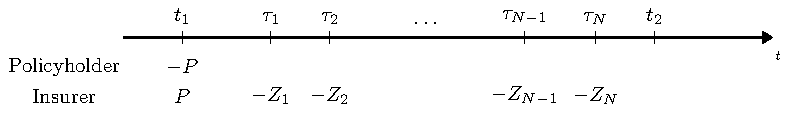
\includegraphics{_main_files/figure-latex/ins-cashflow-1.pdf}
\caption{\label{fig:ins-cashflow}Insurance Contract cash flows.}
\end{figure}

\hypertarget{non-life-insurance-pricing}{%
\section{Non-Life insurance pricing}\label{non-life-insurance-pricing}}

In insurances, the premium that the the insurer offers to the policyholder in exchange for the insurance coverage is not the same for every policyholder. The insurer evaluates the risk related to that policy and determine a ``proper'' premium taking into account risk related factors and commercial related factors. The process of \emph{pricing} corresponds in defining the set of rules for determining this ``proper'' premium \(P_i\) for a specific policyholder \(i\), given the known information on him. In the next sections we are going to better explain what ``proper'' means.

\hypertarget{compound-distribution-hypotheses}{%
\subsection{Compound distribution hypotheses}\label{compound-distribution-hypotheses}}

The first step for evaluating the stochastic process \(\left\{N, Z_1, Z_2, \dots \right\}\) is to introduce some probabilistic hypotheses. The usual hypotheses assumed are the following:

\begin{definition}[Compound distribution]
\label{def:comp-dist} \iffalse (Compound distribution) \fi{}
Let's assume that:

\begin{enumerate}
\def\labelenumi{\arabic{enumi}.}
\tightlist
\item
  for each \(n>0\), the variables \(Z_1|N=n,\ Z_2|N=n,\ \dots,\ Z_n|N=n\) are stochastically independent and identically distributed;
\item
  the probability distribution of \(Z_i|N=n, \ i\le n\) does not depend on \(n\).
\end{enumerate}

Under these hypotheses we say that:
\[
S = \sum_{i=1}^{N}{Z_i}
\]
has a compound distribution.
\end{definition}

The variable \(Z_i|N=n\) used in this definition can be interpreted as the \emph{claim severity for the \(i\)\textsuperscript{th} claim under the hypothesis that \(n\) claims occurred}. The two hypotheses provided in definition \ref{def:comp-dist} imply that the distribution of \(Z_i|N=n, \ i\le n\) does not depend on \(i\) nor on \(n\). For this reason, in the following, we are going to use the notation \(Z\) to represent a random variable with the ditribution of \(Z_i|N=n, \ i\le n\) and \(F_Z(\cdot)\) for its cumulative distribution function (i.e.~\(F_Z(z) = P(Z\le z)\)).

Let's consider the variabile \(Z_i|N\ge i\). We can interpret it as the \emph{claim severity for the \(i\)\textsuperscript{th} claim under the hypothesis that the \(i\)\textsuperscript{th} claim occurred}. From the hypotheses provided in definition \ref{def:comp-dist} we can obtain that also \(Z_i|N\ge i\) has the same distribution of \(Z_i|N=n, \ i\le n\). This can be easily obtained as follows:

\begin{align}
\label{eq:z1}
P\left(Z_i \le z \middle| N\ge i \right) & = P\left(Z_i \le z \middle| \bigvee_{n = i}^{+\infty}{(N=n)}\right)
\\ \label{eq:z2} & =
\sum_{n=i}^{+\infty}{ \underbrace{P\left(Z_i\le z \middle| N=n\right)}_{=F_Z(z)} P\left( N = n \middle| N\ge i \right)}
\\ \label{eq:z3} & =
\sum_{n=i}^{+\infty}{ F_Z(z) P\left( N = n \middle| N\ge i \right)}
\\ \label{eq:z4} & =
F_Z(z) \underbrace{\sum_{n=i}^{+\infty}{P\left( N = n \middle| N\ge i \right)}}_{=1}
\\ \nonumber & =
F_Z(z)
\end{align}

Where:

\begin{itemize}
\tightlist
\item
  the step \eqref{eq:z1} and the step \eqref{eq:z2} are given by the fact that the event \(\{N\ge i\}\) can be decomposed as \(\{N\ge i\} = \left\{ \bigvee_{n = i}^{+\infty}{(N=n)} \right\}\) and that the events \(\{N=n\}, n\in\{i, i+1, i+2, \dots\}\) are two-by-two disjoint, so they constitute a partition of \(\{N\ge i\}\), that allows us to use the disintegrability property of the probability;
\item
  the step \eqref{eq:z3} is due to the fact that the distribution of \(Z_i\le z | N=n\) depends neither on \(i\) nor on \(n\);
\item
  the equivalence \(\sum_{n=i}^{+\infty}{P\left( N = n \middle| N\ge i \right)} = 1\) at step \eqref{eq:z4} is due to the fact that the events \(\{N=n\}, n\in\{i, i+1, i+2, \dots\}\) are a partition of \(\{N\ge i\}\).
\end{itemize}

Therefore, \(Z\) can be considered as the \emph{claim severity for a claim under the hypothesis that that claim occurred}.

\hypertarget{chap:tcc-dist}{%
\subsection{Distribution of the total cost of claims}\label{chap:tcc-dist}}

Under the hypotheses defined in definition \ref{def:comp-dist}, it is possible to obtain the full distribution of \(S\) given the distribution of \(N\) and \(Z\). In this chapter we are going to provide only the formula of the expected value \(E(S)\), but, with the same approach one can obtain all the moments.

The expected value of the total cost of claims \(E(S)\) can be obtained from the expected value of the claims count \(E(N)\) and the expected value of the claim severity \(E(Z)\) as follows:

\begin{align}
\label{eq:s1}
E(S) & = \sum_{n=0}^{+\infty}{P(N=n) \, E\left(S \middle| N = n \right)}
\\ \label{eq:s2} & =
\sum_{n=0}^{+\infty}{P(N=n) \, E\left(\sum_{i=1}^{n}{Z_i} \middle| N = n \right)}
\\ \label{eq:s3} & =
\sum_{n=0}^{+\infty}{P(N=n) \sum_{i=1}^{n}{\underbrace{E\left( Z_i \middle| N = n \right)}_{=E(Z)}}}
\\ \label{eq:s4} & =
\sum_{n=0}^{+\infty}{P(N=n) n E(Z)}
\\ \label{eq:s5} & =
E(Z) \underbrace{\sum_{n=0}^{+\infty}{n P(N=n)}}_{=E(N)}
\\ \label{eq:s6} & =
E(N)E(Z)
\end{align}

Where:

\begin{itemize}
\tightlist
\item
  the step \eqref{eq:s1} is given by the fact that the events \(\{N=0\}, \{N=1\}, \{N=2\}, \dots\) constitute a partition of the certain event \(\Omega\), that allows us to use the disintegrability property of the expected value;
\item
  the step \eqref{eq:s2} is due to the definition of \(S\);
\item
  the step \eqref{eq:s3} is due to the linearity of the expected value;
\item
  the steps \eqref{eq:s4} and \eqref{eq:s5} are due to the fact that, as assumed by the compound distribution hypotheses, \(E\left( Z_i \middle| N = n \right)\) does not depends on \(i\) and \(n\);
\item
  the step \eqref{eq:s6} is due to the definition of the expected value \(E(N)=\sum_{n=0}^{+\infty}{n P(N=n)}\).
\end{itemize}

This result tells us that, under the hypotheses of the compound distribution, it is possible to easily obtain \(E(S)\) from \(E(N)\) and \(E(Z)\). That means that we can model separately \(E(N)\) and \(E(Z)\) and, from them, obtain \(E(S)\). That result is particularly useful in personalization (paragraph \ref{chap:personalization}), because, for each individual \(i\), given the information we have on him, we can estimate his expected claim size \(E(N_i)\) and his expected claim severity \(E(Z_i)\) and obtain his expected total cost of claims as \(E(S_i) = E(N_i) E(Z_i)\).

\hypertarget{chap:risk-prem-tech-price}{%
\subsection{Risk premium and Technical Price}\label{chap:risk-prem-tech-price}}

The expected cost of claims \(E(S)\) is important because it gives us a first interpretation of what ``proper'' premium means.

\begin{definition}[Risk Premium]
\label{def:risk-premium} \iffalse (Risk Premium) \fi{} Said \(S\) the total cost of claims of a policyholder, his \emph{Risk Premium} is given by:
\[
P^{(risk)} = E(S)
\]
\end{definition}

The \emph{Risk Premium} is the premium that on average covers the total cost of claims. As mentioned above, as the coverage spans are usually short, we are not taking into account the timing of the claims so we don't discount the fact that the claims occur later than the premium payment.

It is clear that this premium, that only covers the cost of claims, is not ``proper'' in the practice.

First of all, the insurer has to cover also the expenses related to the policy (commission on sales and expenses related to the claim settlement) and the general expenses of the company. Adding the expenses, we obtain the \emph{Technical Price}.

\begin{definition}[Technical Price]
\label{def:technical-price} \iffalse (Technical Price) \fi{} Said \(S\) the total cost of claims of a policyholder and \(E\) the expenses related to his policy, his \emph{Technical Price} is given by:
\[
P^{(tech)} \ = \ E(S) + E \ = \ P^{(risk)} + E
\]
\end{definition}

Secondly, even if the policyholder paid a premium that on average covers claims and expenses, undertaking that risk with nothing in return would not make sense for the insurer. So, to the Technical Price, some further loadings must be added, as for example risk margin and profit margin.

The amount of the Technical Price with these loadings can be further modified based on business logic, as we are going to discuss later.

\hypertarget{chap:personalization}{%
\section{Modeling and Personalization}\label{chap:personalization}}

In this section we are going to better explain how pricing based on policyholder information works.

\hypertarget{chap:pricing-variables}{%
\subsection{Pricing variables}\label{chap:pricing-variables}}

Usually for every policyholder we have a certain amount of information on him that is considered relevant for his risk evaluation. This information must be reliable and observable at the moment of the underwriting of the policy.

In motor insurances, this information could be:

\begin{itemize}
\tightlist
\item
  Information on the insured vehicle: make, model, engine power, vehicle mass, age of the vehicle;
\item
  General information of the policyholder: age, sex, address (region, city, postcode), ownership of a private box where he parks the car;
\item
  Insurance specific information of the policyholder: number of claims caused in the previous years, how long he has been covered, bonus-malus class;
\item
  Policy options: amount of the maximum coverage, presence and amount of a deductible, presence of other insurance guarantees, how many drivers will drive the vehicle;
\item
  Customer information on the policyholder: how many years he has been a customer of the insurer, how many other policies he owns.
\item
  Telematic data: how many kilometers per year the policyholder travelled in the previous years, how many sharp accelerations and decelerations per kilometer the policyholder performed in the previous years.
\end{itemize}

These pieces of information are usually called \emph{pricing variables}.

We must observe that some of these variables are available for every potential customer (such as his age and address), while others are only available for policyholder that are already customers (such as telematic data that is available only if the policyholder agreed on installing on their car the device that collects this data).

Moreover, even considering the variables that are available for every customer, it is important to be aware on how reliable they are. Some of them comes from official documents (as customer age and address or bonus-malus class), but others could be declared by the customer and his statements are not easily verifiable by the insurer (as the ownership of a private box or how many drivers will drive the vehicle).

This topic of variables reliability fits in the wider framework of fraud detection. Insurance companies put a lot of effort in preventing frauds. This is done with active actions, such as documents checks and inspections, and with predictive fraud detections models. The two most common categories of frauds are underwriting frauds (such as false declaration on insurance related data) and settlement frauds (such as faking an accident). The customer information on the policyholder is usually important to predict both underwriting frauds and settlement frauds. Usually customers that have a longer relationship with the company and own many policies are less likely to commit frauds.

Regarding the topic of variables reliability, the Italian Insurance Associations (\href{https://www.ania.it/}{ANIA}) in the last years made some big steps forward by collecting in its databases a lot of information about policyholders and vehicles and making it available to insurance companies. For example, by logging in these databases it is possible, at the moment of the quote request, to retrieve useful insurance specific information such as the number of claims caused by the customer in the previous years or how long he has been covered and useful information on his vehicle such as when it has been registered or how many changes of ownership did it experienced.

One of the roles of the actuary is to understand how reliable the information on the policyholder is and to decide how to use that information.

\hypertarget{chap:pricing-variables-encoding}{%
\subsection{Pricing variables encoding}\label{chap:pricing-variables-encoding}}

Formally the pricing variables can be encoded as a vector of real numbers. \(\boldsymbol{x}_i=(x_{i1}, x_{i2}, \dots, x_{ip})\in\mathcal{X}\subseteq\mathbb{R}^p\). In the modeling framework they can be also called explanatory variables, covariates, predictors or features.

The pricing variables can be of two types:

\begin{enumerate}
\def\labelenumi{\arabic{enumi}.}
\tightlist
\item
  \emph{Quantitative variables}: variables, like policyholder age or vehicle mass, that can be easily represented as a number;
\item
  \emph{Qualitative variables}: variables, like policyholder sex or vehicle make, that represent a category and are usually represented with strings.
\end{enumerate}

The quantitative variables, with eventual transformations, are already suitable to be used.

To facilitate the use of the qualitative variables, they are usually encoded as sets of binary variables.

If a variable \(x\) has only 2 possible modalities, it can be easily encoded in a binary variable \(x'\) that assigns \(0\) to one modality and \(1\) to the other. For example, if \(x = \text{sex}\), it can be encoded this way:
\[
x' = \begin{cases}
1 & \text{if } \text{sex } = \text{ `Male'} \\
0 & \text{if } \text{sex } = \text{ `Female'}
\end{cases}
\]

In general, if a variable \(x\) has \(K\) modalities, it can be encoded in \(K-1\) binary variables \(x'_1, x'_2, \dots, x'_{K-1}\). For example, if \(x = \text{make}\) and it can have 4 possible modalities (`Fiat', `Alfa-Romeo', `Lancia', `Ferrari') it can be encoded this way:
\begin{align*}
x'_1 & = \begin{cases}
1 & \text{if } \text{make } = \text{ `Fiat'} \\
0 & \text{otherwise} \\
\end{cases}
\\
x'_2 & = \begin{cases}
1 & \text{if } \text{make } = \text{ `Alfa-Romeo'} \\
0 & \text{otherwise} \\
\end{cases}
\\
x'_3 & = \begin{cases}
1 & \text{if } \text{make } = \text{ `Lancia'} \\
0 & \text{otherwise} \\
\end{cases}
\\
\end{align*}

The variables \(x'_1\), \(x'_2\), \(x'_3\) are called dummy variables. We can observe that all the information about the make is embedded in just these 3 variables, so a fourth dummy variable that indicate the modality `Ferrari' is not needed. Indeed:
\[
\text{make } = \text{`Ferrari'} \ \Longleftrightarrow \ x'_1=x'_2=x'_3=0
\]
In table \ref{tab:dummy-variables} the dummy variable encoding is illustrated.

\begin{table}[!h]

\caption{\label{tab:dummy-variables}Dummy variables encoding.}
\centering
\begin{tabular}[t]{lccc}

\textbf{Make} & \textbf{$x'_1$} & \textbf{$x'_2$} & \textbf{$x'_3$}\\
\midrule\addlinespace
Fiat & 1 & 0 & 0\\
Alfa-Romeo & 0 & 1 & 0\\
Lancia & 0 & 0 & 1\\
Ferrari & 0 & 0 & 0\\

\end{tabular}
\end{table}

For some models it is suggested to use also the dummy variable that indicates the \(K\)\textsuperscript{th} modality. This encoding is called one-hot encoding and it is mainly used in Neural Networks. For the models considered in this paper the \(K-1\) dummy variables encoding is preferred, so we will always consider it.

In the following, when we use the notation \(\boldsymbol{x}_i=(x_{i1}, x_{i2}, \dots, x_{ip})\), I'll always consider that the qualitative variables have been already encoded as dummy variables, so \((x_{i1}, x_{i2}, \dots, x_{ip})\in \mathcal{X} \subseteq \mathbb{R}^p\)

\hypertarget{pricing-rule-and-modeling}{%
\subsection{Pricing Rule and Modeling}\label{pricing-rule-and-modeling}}

The pricing variables are used as input of a \emph{Pricing Rule}.

\begin{definition}[Pricing Rule]
\label{def:pricing-rule} \iffalse (Pricing Rule) \fi{} A \emph{Pricing Rule} is a function \(f(\cdot)\) that from an instance of a set of pricing variables \(\boldsymbol{x}_i\in\mathcal{X}\) returns a price:

\[  
\begin{array}{rccl}
f: & \mathcal{X}      & \longrightarrow  & R_+ \\
   & \boldsymbol{x}_i & \longmapsto      & P_i \\
\end{array}
\]
\end{definition}

The process of pricing consists in defining a Pricing Rule based on observed data from the past and assumptions on the future.

The first step for defining a Pricing Rule is to model the total cost of claims \(S\) and obtain a pricing rule for the risk premium \(P^{(risk)}\).

\begin{definition}[Modeling]
\label{def:modeling} \iffalse (Modeling) \fi{} Modeling a \emph{response variable} \(Y\) means finding a function
\[r:\mathcal{X}\rightarrow \mathcal{C}\]
that, given a set of explanatory variables \(\boldsymbol{x}_i=(x_{i1}, x_{i2}, \dots, x_{ip})\in \mathcal{X} \subseteq \mathbb{R}^p\), returns the expected value of the response variable \(E(Y)\) and possibly other moments of \(Y\) or even the full distribution of \(Y\).
\end{definition}

In definition \ref{def:modeling} we used a generic \(\mathcal{C}\) as codomain of the function \(r(\cdot)\) to not specify whether the model describes just \(E(Y)\) (and so \(\mathcal{C}=\mathbb{R}\)) or something more, such as the couple \(\left( E(Y), Var(Y) \right)\) or the full distribution of \(Y\).

As we observed in section \ref{chap:tcc-dist}, under the compound distribution hypotheses, it is not needed to model directly the total cost of claims \(S\), but we can separately model \(N\) and \(Z\).

\hypertarget{response-variables-and-distributions}{%
\subsection{Response variables and distributions}\label{response-variables-and-distributions}}

Usually in statistical modeling, the response variables are seen as random variables with a distribution belonging to a specified family.

\hypertarget{chap:dist-n}{%
\subsubsection{\texorpdfstring{Distribution for the claims count \(N\)}{Distribution for the claims count N}}\label{chap:dist-n}}

The claim count \(N\) is a discrete variable with values in \(\{0, 1, 2, 3,\dots\}\). Even if in practice the number of claims can't be arbitrarily high, \(N\) is usually modeled with distributions that give a positive probability to all natural numbers. One of the most common distribution used for \(N\) is the Poisson distribution.

\begin{definition}[Poisson Distribution]
\label{def:def-poisson} \iffalse (Poisson Distribution) \fi{} A random variable \(N\) with support \(\{0,1,2,3,\dots \}\) has a Poisson distribution, if its probability function is:
\[
p_N(n) = P\left( N = n \right) = e^{-\lambda}\frac{\lambda^n}{n!}, \quad \lambda>0
\]
We will indicate it with the notation \(N \sim Poisson(\lambda)\).
\end{definition}

\begin{figure}[!hbtp]

{\centering 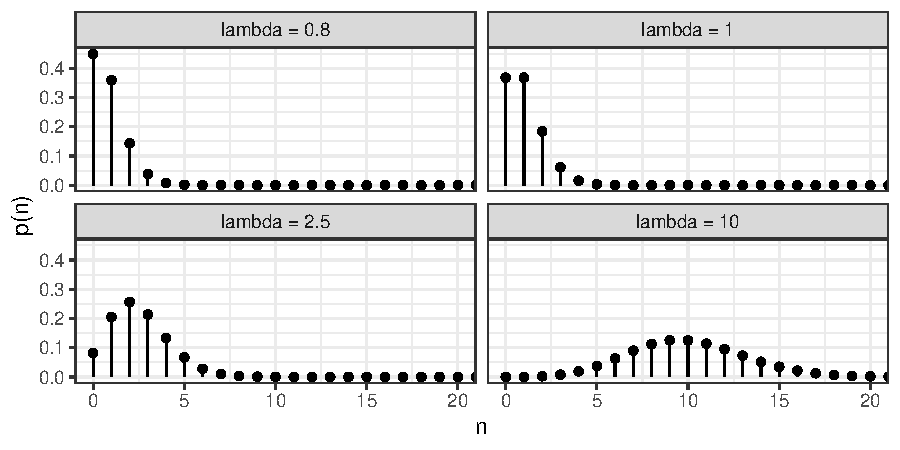
\includegraphics[width=0.9\linewidth]{_main_files/figure-latex/plot-poisson-1} 

}

\caption{Poisson distribution for some values of $\lambda$.}\label{fig:plot-poisson}
\end{figure}

The Poisson distribution is a parametric distribution that only depends on the parameter \(\lambda\). In figure \ref{fig:plot-poisson}, for different levels of \(\lambda\) the distribution is represented. These plots show how for larger values of \(\lambda\), the distribution is shifted to larger values and it is wider.

Indeed, the first two moments are:
\begin{align*}
E(N)   & = \lambda \\
Var(N) & = \lambda
\end{align*}

Thus, increasing \(\lambda\), both \(E(N)\) and \(Var(N)\) increase.

Looking to the distribution shape, we can see that:

\begin{itemize}
\tightlist
\item
  if \(\lambda<1\), the mode is in \(n=0\);
\item
  if \(\lambda=1\), \(p(0)=p(1)=\frac{1}{e}\);
\item
  if \(\lambda>1\), the mode is in a value greater than \(0\) and, as \(\lambda\) increases, the distribution assumes a bell shape similar to the Normal distribution one. The convergence to the Normal distribution can be obtained with the \emph{Central Limit Theorem}.
\end{itemize}

In non-life insurance we usually are in the case with \(\lambda<1\). E.g. the average number of claims for motor third party liability insurances in Italy, in 2018 has been 5.68\%\footnote{\href{https://www.ania.it/ricerca-avanzata/-/asset_publisher/XIyLeujL9irt/content/id/113283}{ANIA yearly statistical report for motor third party liability}}.

The property \(Var(N) = E(N)\) is an important constraint when the distribution is used in practice. It is possible that the observed data shows a different pattern. Often the observed data shows a situation where \(Var(N) > E(N)\). This phenomenon is called \emph{overdispersion}.

To address this issue it is possible to use more flexible distributions, such as Negative-Binomial distribution, or to adopt less assumptions on the response variable distribution. One common technique is the assumption of Quasi-Poisson distribution, that we will describe in chapter \ref{chap:models}.

\hypertarget{chap:exposure}{%
\subsubsection{Exposure}\label{chap:exposure}}

In section \ref{chap:non-life-ins} we said that non-life insurances usually have a fixed coverage period that usually spans for one year. Often we work with portfolios of insurances with different coverage periods. For example, this could be due to the presence of insurances born with shorter coverage periods or to the presence of insurances that has been closed earlier. Moreover, in companies data, often insurance data are collected for accounting years. This means that, if an insurance coverage \(c\) spans in two consecutive years \(a\) and \(a+1\), it is collected as two records: the couple \((c, a)\) and the couple \((c, a+1)\). This situation is quite common, as usually coverages start during the year and not all at the first of the year.

The coverage span for an insurance coverage is called \emph{exposure} and it is usually measured in years-at-risk. For instance, if an insurance coverage spans for 3 months, it corresponds to a quarter of year, so the exposure, measured in years-at-risk, is \(v=\frac{1}{4}\). The term year-at-risk comes from the fact that the policyholder exposure is a risk for the insurer, so the exposure is the period in which the insurer is exposed to the risk of paying claims.

It is natural to assume that, if a policyholder has a longer exposure, it is expected for him to experience more claims. Considering that we have to work with policies with different exposures, in order to take this aspect into account, the usual assumption taken in the following. Said \(M\) the number of claims the policyholder will experience during his period of exposure \(v\) (measured in years) and \(N\) the number of claims the policyholder would experience during one year, we assume \(E(M) = v E(N)\).

This assumption can be further extended if we assume that the claims come from a \emph{Poisson process}.

\begin{definition}[Counting Process]
\label{def:def-process-count} \iffalse (Counting Process) \fi{} A stocastic process \(\{N(t), t\ge0\}\) is called \textit{counting process} if:

\begin{enumerate}
\item The determination of N(t) are natural numbers \\
      $N(t) \in \{ 0, 1, 2, ... \} \ t\ge 0$
\item The process is not decreasing \\
      $s < t \Rightarrow N(s) \le N(t)$
\end{enumerate}
\end{definition}

In a counting process \(\{N(t), t\ge0\}\):

\begin{itemize}
\tightlist
\item
  \(N(t)\) can be interpreted as the number of events or arrivals that occur in the period \([0, t]\);
\item
  \(N(t) - N(s), \ s\le t\) can be interpreted as the number of events or arrivals that occur in the period \(]s, t]\). \(N(t) - N(s)\) is also called \emph{increment} of the process.
\end{itemize}

The counting process can be used to model the number of claims that occur to a specific policy.

\begin{definition}[Poisson Process]
\label{def:def-process-poisson} \iffalse (Poisson Process) \fi{} A counting process \(\{N(t), t\ge0\}\) is a \textit{Poisson process} with intensity \(\lambda\) if:

\begin{enumerate}
\item The increments of the process are stocastically independent \\
      $\forall n\ge0, \forall s_1 < t_1 \le \dots \le s_n < t_n$ \\
      $\Rightarrow \ N(t_1)-N(s_1), \dots, N(t_n)-N(s_n)$ are stocastically independent;
\item The probability of arrival in an interval is proportional to the size of the interval \\
      $\forall t\ge 0, \forall \Delta t >0 \ \Rightarrow \ P\left( N(t + \Delta t) - N(t) = 1 \right) = \lambda \Delta t + \omicron (\Delta t)$ \\
      where $\lim_{\Delta t \to 0}{\frac{\omicron(\Delta t)}{\Delta t}} = 0$
\item Multiple arrivals are excluded \\
      $\forall t\ge 0, \forall \Delta t >0 \ \Rightarrow \ P\left( N(t + \Delta t) - N(t) \ge 2 \right) = \omicron (\Delta t)$
\item Arrivals at time $0$ are almost impossible \\
      $P\left( N(0) = 0 \right) = 1 $
\end{enumerate}
\end{definition}

Under these hypotheses we obtain the following result:

\begin{theorem}[Poisson Process]
\label{thm:th-process-poisson} \iffalse (Poisson Process) \fi{} If \(\{N(t), t\ge 0 \}\) is a Poisson process with intensity \(\lambda\), then:
\[\forall t\ge 0, \forall \Delta t >0, \ \Rightarrow \ N(t + \Delta t) - N(t) \sim Poisson(\lambda \Delta t)\]
\end{theorem}

This result tells us that the distribution of the number of events in any interval \(]t, t+\Delta t]\) only depends on the size of the interval \(\Delta t\). Moreover, for the Poisson property we saw in section \ref{chap:dist-n}, we get:
\[E(N(t + \Delta t) - N(t)) = \lambda \Delta t\]

So, the expected number of arrivals is proportional to the size of the interval \(\Delta t\). The intensity of the process \(\lambda\) can be also interpreted as the expected number of claims in a unit period.

If we assume that the claims that occur to a policy come from a Poisson process with intensity \(\lambda\), if we observe that policy for the period \(]t, t+v]\), the claims count in that exposure period \(M\) are distributed as:
\[ M\sim Poisson(v \lambda) \]
In particular, if the observed period spans 1 year, we get:
\[ M = N \sim Poisson(\lambda) \]

\hypertarget{distribution-for-the-claim-severity-z}{%
\subsubsection{\texorpdfstring{Distribution for the claim severity \(Z\)}{Distribution for the claim severity Z}}\label{distribution-for-the-claim-severity-z}}

The claim severity \(Z\) is a continuous variable with values in \([0, +\infty[\). As for the claims count \(N\), even if in practice it can't be arbitrarily high, it is usually modeled with distributions that give a positive density to all the numbers in \(]0, +\infty[\). As the null claims are excluded, it is natural to assume \(P\left( Z=0 \right) = 0\). One of the most common distribution used for \(Z\) is the Gamma distribution.

\begin{definition}[Gamma Distribution]
\label{def:def-gamma} \iffalse (Gamma Distribution) \fi{} A random variable \(Z\) with support \([0, +\infty[\) has a Gamma distribution, if its probability density function is:
\[
f_Z(z) = \frac{\rho^\alpha}{\Gamma(\alpha)}z^{\alpha-1}e^{-\rho z}, \quad \alpha > 0, \ \rho > 0
\]
where \(\Gamma(\alpha) = \int_{0}^{+\infty}{z^{\alpha - 1} e^{-z} \mathrm{d} z}\).

We will indicate it with the notation \(Z \sim Gamma(\alpha, \rho)\).
\end{definition}

\begin{figure}[!hbtp]

{\centering 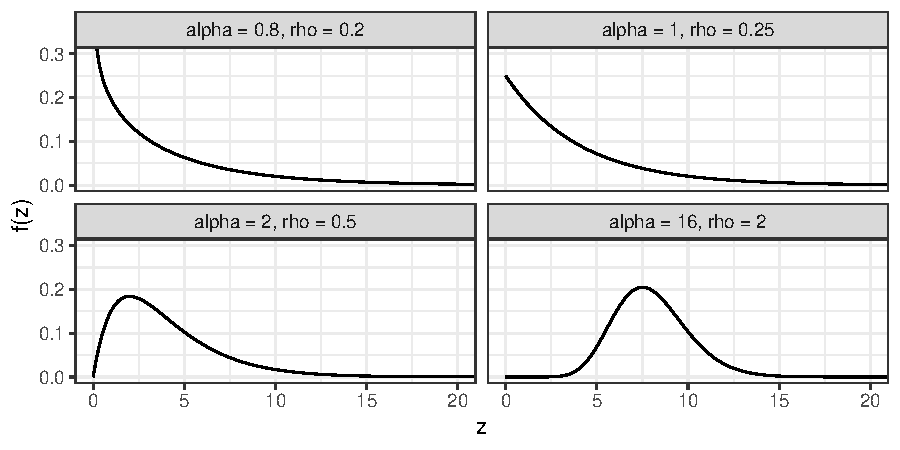
\includegraphics[width=0.9\linewidth]{_main_files/figure-latex/plot-gamma-1} 

}

\caption{Gamma distribution for some values of $\alpha$ and $\rho$.}\label{fig:plot-gamma}
\end{figure}

The Gamma distribution is a parametric distribution that depends on two parameters:

\begin{itemize}
\tightlist
\item
  \(\alpha > 0\), called shape parameter
\item
  \(\rho > 0\), called scale parameter
\end{itemize}

The first two moments of the Gamma distribution are:
\begin{align*}
E(Z)   & = \frac{\alpha}{\rho} \\
Var(Z) & = \frac{\alpha}{\rho^2}
\end{align*}

In figure \ref{fig:plot-gamma}, for different levels of \(\alpha\) and \(\gamma\) the distribution is represented. These plots show how changing the values of \(\alpha\) and \(\gamma\), the shape changes. We can see that:

\begin{itemize}
\tightlist
\item
  if \(\alpha < 1\), \(f_z(\cdot)\) is not defined in \(0\) and it has a vertical asymptote in \(z = 0\). In \(]0, +\infty]\) it is monotonically decreasing.
\item
  if \(\alpha = 1\), \(f_z(\cdot)\) starts from \(f(0) = \rho\) and then decreases monotonically. In this case, the density function becomes \(f_z(z) = \rho e^{-\rho z}\) and the distribution is also called exponential distribution.
\item
  if \(\alpha > 0\), \(f_z(\cdot)\) starts from \(f(0) = 0\), increases until the mode and then decreases.
\end{itemize}

In figure \ref{fig:plot-gamma} the first three distributions represented have the same expected value \(E(Z)=\frac{\alpha}{\rho} = 4\), but different shapes. The third and the fourth have the same variance \(Var(Z) = \frac{\alpha}{\rho^2} = 8\), but different expected values. As the shape parameter \(\alpha\) increases, the distribution assumes a bell shape similar to the Normal distribution one. The convergence to the Normal distribution can be obtained with the \emph{Central Limit Theorem}.

Another parametrization often used for Gamma distribution is obtained by using the mean \(\mu\) as a parameter:
\[
\mu = \frac{\alpha}{\rho}
\]
With this parametrization, the density function becomes:
\[
f_Z(z) = \frac{\left(\frac{\alpha}{\mu}\right)^\alpha}{\Gamma(\alpha)}z^{\alpha-1}e^{-\frac{\alpha}{\mu} z}, \quad \alpha > 0, \ \rho > 0
\]

The advantage of using the parameters \((\alpha, \mu)\) is that the link between \(E(Z)\) and \(Var(Z)\) becomes clearer:
\begin{align*}
E(Z)   & = \mu \\
Var(Z) & = \frac{1}{\alpha}\mu^2
\end{align*}

Computing the coefficient of variation we then obtain:
\[CV(Z) = \frac{\sqrt{Var(Z)}}{E(Z)} = \frac{1}{\sqrt{\alpha}}\]
This result means that the coefficient of variation is constant (given the shape parameter \(\alpha\)). As we saw for the Poisson distribution, it is possible that observed data shows a different pattern. In chapter \ref{chap:models}, for the Gamma distribution, we will use the parametrization based on \((\alpha, \mu)\) instead of the one based on \((\alpha, \rho)\).

Another characteristic of Gamma distribution that could be problematic in modeling claims severity is that it has a light tail. This means that, as \(z\) goes to \(+\infty\), \(f_Z(z)\) aproaches \(0\) quite fast. This could lead to a poor fitting for \emph{large claims}. Other distributions with havier tails are for example the \emph{log-Normal} and the \emph{Pareto}.

\hypertarget{chap:large-claims}{%
\subsubsection{Large claims}\label{chap:large-claims}}

Modeling large claims in quite difficult in practice because usually there is not a lot of observed data on them, so it is hard to understand if they are related to some risk factors (identifiable by the pricing variables) or they happen just by chance.

First of all, to model large claims, we must define what a large claim is. What is usually done in practice is just choosing a threshold \(\bar{z}\) and considering large all the claims with a size that exceeds that threshold. The value \(\bar{z}\) must be chosen sufficiently big to consider large the claims above \(\bar{z}\), but not so big that there are not enough observed claims that exceeds \(\bar{z}\). One common choice for Motor Third Party Liability in European markets could be \(\bar{z} = 100' 000 \text{\euro}\).

\begin{definition}[Large and Attritional Claims]
\label{def:def-large-claim} \iffalse (Large and Attritional Claims) \fi{} Given a predetermined threshold \(\bar{z}\), we say that:

\begin{itemize}
\item a claim $Z$ is a \textit{large claim} if $Z > \bar{z}$
\item a claim $Z$ is an \textit{attritional claim} if $Z \le \bar{z}$
\end{itemize}

For each claim \(Z\) we call:

\begin{itemize}
\item \textit{Capped Claim Size} \\
      $Z' = \min(Z, \bar{z})$;
\item \textit{Excess Over the Threshold} \\
      $Z'' = \max(Z - \bar{z}, 0)$.
\end{itemize}
\end{definition}

In figure \ref{fig:large-claim} the \emph{Capped Claim Size} and the \emph{Excess Over the Threshold} are shown. It is easy to show that \(Z\) can be decomposed as:
\[Z = Z' + Z''\]

\begin{figure}
\centering
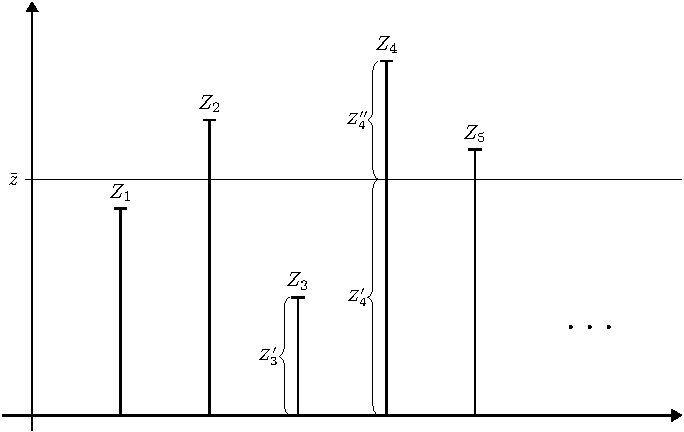
\includegraphics{_main_files/figure-latex/large-claim-1.pdf}
\caption{\label{fig:large-claim}Large claims.}
\end{figure}

Given the total number of claims \(N\), it can be decomposed as:
\[N = N^{(a)} + N^{(l)}\]
where

\begin{itemize}
\tightlist
\item
  \(N^{(a)}\) is the attritional claims count, i.e.~the number of claims with size \(Z \le \bar{z}\);
\item
  \(N^{(l)}\) is the large claims count, i.e.~the number of claims with size \(Z > \bar{z}\);
\end{itemize}

Let's indicate with \(Z_{(i)}\) the \(i\)\textsuperscript{th} in order from the smallest to the bigger. Sorting the claims we can separate the attritional claims from the large claims as follows:
\[
\underbrace{Z_{(1)}, Z_{(2)}, \dots, Z_{(N^{(a)})}}_{\text{Attritional Claims}},
\underbrace{Z_{(N^{(a)} + 1)}, Z_{(N^{(a)} + 2)}, \dots Z_{(N^{(a)} + N^{(l)})}}_{\text{Large Claims}}
\]

In order to model the large claims it is possible to use the following three decompositions of the total cost of claims \(S\):
\begin{align}
  \nonumber
  S & = \underbrace{Z_{(1)} + Z_{(2)} + \dots + Z_{(N^{(a)})}}_{\text{Attritional Claims}} +
        \underbrace{Z_{(N^{(a)} + 1)} + Z_{(N^{(a)} + 2)} + \dots Z_{(N^{(a)} + N^{(l)})}}_{\text{Large Claims}} \\
  \label{large-claim-decomposition-1}
    & = \underbrace{\sum_{i=1}^{N^{(a)}}{Z_{(i)}}}_{=S^{(a)}} +
            \underbrace{\sum_{i = N^{(a)} + 1}^{N^{(a)} + N^{(l)}}{Z_{(i)}}}_{=S^{(l)}}
    \ = \ S^{(a)} + S^{(l)} \\[12pt]
  \label{large-claim-decomposition-2}
  S & = \sum_{i=1}^{N}{Z_i}
    \ = \ \sum_{i=1}^{N}{\left(
      %\{Z_i|Z_i>\bar{z}\} I_{Z_i>\bar{z}} +
      %\{Z_i|Z_i\le\bar{z}\} I_{Z_i\le\bar{z}}
      Z_i I_{Z_i>\bar{z}} +
      Z_i I_{Z_i\le\bar{z}}
      \right)} \\[12pt]
  \label{large-claim-decomposition-3}
  S & = \sum_{i=1}^{N}{Z_i}
    \ = \ \sum_{i=1}^{N}{\left(Z'_i + Z''_i\right)}
    \ = \ \sum_{i=1}^{N}{\left(Z'_i + Z''_i I_{Z_i > \bar{z}}\right)}
\end{align}

These three decompositions of \(S\) are useful because they provide three decompositions of \(E(S)\):
\begin{align}
  \nonumber
  E(S) & = E(S^{(a)}) + E(S^{(l)}) \\
    \label{large-claim-decomposition-expected-1}
    & = E(N^{(a)}) E(Z|Z\le\bar{z}) + E(N^{(l)}) E(Z|Z>\bar{z}) \\[12pt]
  \nonumber
  E(S) & = E(N) E(Z) \\
    \nonumber
    & = E(N) \left[P(Z\le\bar{z}) E(Z|Z\le\bar{z}) + P(Z>\bar{z}) E(Z|Z > \bar{z}) \right] \\
    \label{large-claim-decomposition-expected-2}
    & = E(N) \left[\left( 1 - P(Z>\bar{z}) \right) E(Z|Z\le\bar{z}) + P(Z>\bar{z}) E(Z|Z > \bar{z})\right] \\[12pt]
  \nonumber
  E(S) & = E(N) E(Z) \\
    \label{large-claim-decomposition-expected-3}
    & = E(N) \left[E(Z') + P(Z>\bar{z}) E(Z'')\right]
\end{align}

\ref{large-claim-decomposition-expected-1}, \ref{large-claim-decomposition-expected-2} and \ref{large-claim-decomposition-expected-3} provide three approaches to model attritional and large claims.

\begin{enumerate}
\def\labelenumi{\arabic{enumi}.}
\tightlist
\item
  Looking to \ref{large-claim-decomposition-expected-1} we can model separately attritional claims and large claims. Modeling \(N^{(a)}\) and \(Z|Z\le\bar{z}\) we estimate the total cost of claims for the attritional part \(S^{(a)}\); modeling \(N^{(l)}\) and \(Z|Z>\bar{z}\) we estimate the total cost of claims for the large part \(S^{(l)}\).
\item
  Looking to \ref{large-claim-decomposition-expected-2} we can model together the claim count \(N\), and then we can model the cost of the attritional claims \(Z|Z\le\bar{z}\), the cost of the large claims \(Z|Z>\bar{z}\) and the probability to exceed the threshold \(P(Z>\bar{z})\).
\item
  Looking to \ref{large-claim-decomposition-expected-3} we can model together the claim count \(N\), and then we can model the capped claims size \(Z'\), the excess over the threshold \(Z''\) and the probability to exceed the threshold \(P(Z>\bar{z})\).
\end{enumerate}

If the large claims component weighs a lot on the total cost of claims, these approaches could lead to quite different estimates of \(E(S)\). In particular, if in the observed data the number of large claims is small, it will be hard to model both \(N^{(l)}\) and \(P(Z>\bar{z})\), so for these components the modeling process could lead to a flat model (i.e.~a model without any explanatory variable) or almost flat one (i.e.~a model with just few explanatory variables and with mild effects). However, with the first approach, a flat model for \(N^{(l)}\) leads to distribute the observed total cost of large claims proportionally to all the policies, while with the second and the third, a flat model for \(P(Z>\bar{z})\) leads to distribute the observed total cost of large claims proportionally to the expected number of claims \(E(N)\). So, with the first approach, a flat model brings to more solidarity between policies, while, with the second approach, a flat model could bring to an exacerbation of the differences identified by modeling \(N\).

For the second approach we must also introduce a distribution suitable for modeling \(P(Z>\bar{z})\).

\hypertarget{binomial-distribution}{%
\subsubsection{Binomial distribution}\label{binomial-distribution}}

The \emph{binomial distribution} is used to model the counting on events that occurs (successes) in a fixed amount of trials \(n\). For example we can use it to model the number of large claims within a fixed number of \(n\) claims.

\begin{definition}[Binomial Distribution]
\label{def:def-binomial} \iffalse (Binomial Distribution) \fi{} A random variable \(Y\) with support \(\{0,1,2, \dots, n \}\) has a Binomial distribution, if its probability function is:
\[
p_Y(y) = P\left( Y = y \right) = \binom{n}{y} p^y (1-p)^{n-y}, \quad p \in [0, 1]
\]
We will indicate it with the notation \(Y \sim Binom(n, p)\).
\end{definition}

\begin{figure}[!hbtp]

{\centering 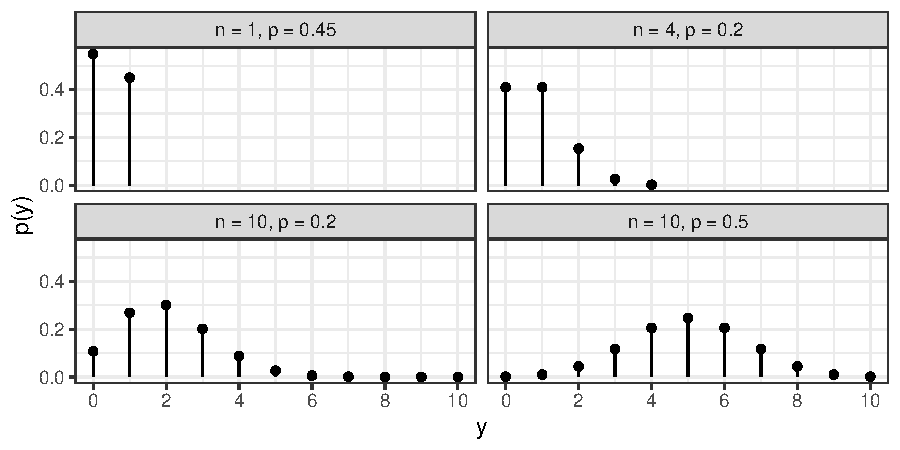
\includegraphics[width=0.9\linewidth]{_main_files/figure-latex/plot-binomial-1} 

}

\caption{Binomial distribution for some values of $n$ and $p$.}\label{fig:plot-binomial}
\end{figure}

The binomial distribution is a parametric distribution that depends on the parameters \(n\) and \(p\). \(n\) represents the number of trials, while \(p\) represents the probability for a trial to succed. The assumption is that the \(n\) trials are identical, so they have all the same probability \(p\) to succed. In figure \ref{fig:plot-binomial} the distribution is represented for different levels of \(n\) and \(p\).

The first two moments of the binomial distribution are:
\begin{align*}
E(N)   & = np \\
Var(N) & = np(1-p)
\end{align*}

If \(n = 1\), the binomial distribution assumes only the values \(1\) (with probability \(p\)) and \(0\) (with probability \(1-p\)). In this case it is also called \emph{Bernoullian distribution} and it can be used to model the indicator of an event \(I_E\).

If \(n>1\), the binomial distribution assumes a shape centered on its expected value \(E(Y)=np\) and fading for values of \(y\) that moves away from \(E(Y)\). As \(n\) increases, the distribution assumes a bell shape similar to the Normal distribution one. The convergence to the Normal distribution can be obtained with the \emph{Central Limit Theorem}.

From the binomial Distribution it is also possible to define the scaled binomial distribution by dividing its value by \(n\).

\begin{definition}[Scaled Binomial Distribution]
\label{def:def-scaled-binomial} \iffalse (Scaled Binomial Distribution) \fi{} If \(Y\sim Binom(n, p)\), and \(Y' = \frac{Y}{n}\), we will say that \(Y'\) has a \textit{Scaled Binomial Distribution} and we will indicate it with the notation \(Y' \sim Binom(n, p)/n\).

The support of \(Y'\) is \(\{0, \frac{1}{n}, \frac{2}{n}, \dots, 1 \}\) and its probability function is:
\[
p_{Y'}(y') = P\left( Y' = y' \right) = \binom{n}{ny'} p^{ny'} (1-p)^{n-ny'}, \quad p \in [0, 1]
\]
\end{definition}

In chapter \ref{chap:models} we will use the Scaled Binomial Distribution.

In non-life insurance pricing, the binomial distribution can be used to model the probability for a claim to have specific characteristics. For example we can use it to model the probability that a certain claim is a large one, \(P(Z>\bar{z})\), in order to model separately attritional claims severity \(\{Z|Z\le\bar{z}\}\) and large claims severity \(\{Z|Z>\bar{z}\}\), as we have seen in section \ref{chap:large-claims}.

Another example is the decomposition between claims with only material damages and claims with also bodily injuries. Modeling separately these two components is useful because they usually have a different distribution for the claim size.

As for large claims we can decompose \(S\) in the following two ways:
\begin{align}
  \nonumber
  E(S) & = E(S^{(things)}) + E(S^{(inj)}) \\
    \label{inj-claim-decomposition-expected-1}
    & = E(N^{(things)}) E(Z|\bar{J}) + E(N^{(inj)}) E(Z|J) \\[12pt]
  \nonumber
  E(S) & = E(N) E(Z) \\
    \nonumber
    & = E(N) \left[P(\bar{J}) E(Z|\bar{J}) + P(J) E(Z|J) \right] \\
    \label{inj-claim-decomposition-expected-2}
    & = E(N) \left[\left( 1 - P(J) \right) E(Z|\bar{J}) + P(J) E(Z|J)\right]
\end{align}
where:

\begin{itemize}
\tightlist
\item
  \(N^{(things)}\) is the number of claims with only material damages;
\item
  \(N^{(inj)}\) is the number of claims with injuries;
\item
  \(J\) is the event that represents that a specific claim presents injuries; such as \(Z\) is a representative for \(Z_1, Z_2, \dots, Z_N\), \(J\) is a representative for \(J_1, J_2, \dots, J_N\).
\end{itemize}

Combining this decomposition with what we have seen in large claims decomposition, we can further develop our decomposition taking into account both the presence or absence of injuries and the occurrence or not of a large claim. One example could be:
\begin{align*}
E(S) & = E(N) \left[\left( 1 - P(J) \right) E(Z|\bar{J}) + P(J) E(Z|J) \right] \\[4pt]
  & = E(N) \left\{ \right. \\
  & \qquad \left( 1 - P(J) \right) E(Z|\bar{J}) \\
  & \qquad + P(J) \left[ \right. \\
  & \qquad \qquad P(Z \le \bar{z} | J) E\left( Z \mid Z\le \bar{z} \land J \right) \\
  & \qquad \qquad + P(Z < \bar{z} | J) E\left( Z \mid Z < \bar{z} \land J \right) \\
  & \qquad \left. \right] \\
  & \quad \left. \right\}
\end{align*}

This way, we are decomposing only the claims with injuries between attritional and large. That makes sense because claims that don't produce injuries usually have small severities.

\hypertarget{model-fitting-and-data-available}{%
\subsection{Model fitting and data available}\label{model-fitting-and-data-available}}

Once we have chosen how to decompose \(S\), we have to model the response variables needed for that decomposition (\(N\), \(Z\), \(I_J\), \ldots) with the explanatory variables. Thus we have to estimate a function \(r:\mathcal{X}\rightarrow \mathcal{C}\) as defined in \ref{def:modeling}.

In order to estimate \(r(\cdot)\) we have also to take some assumptions on the distribution of the response variable and on the shape of \(r(\cdot)\). We will call \emph{model} a set of assumptions on the response variable and on the shape of \(r(\cdot)\). We will discuss some of the most widespread models for claims count and claims severity in chapter \ref{chap:models}.

Defined the model, we have to estimate it using observed data. In general, to model a response variable \(Y_i\) with the explanatory variables \(\boldsymbol{x}_i=(x_{i1}, x_{i2}, \dots, x_{ip})\in \mathcal{X} \subseteq \mathbb{R}^p\), the observed data is in the form:
\[
\mathcal{D} = \left\{(\boldsymbol{x}_1, w_1, y_1), \ (\boldsymbol{x}_2, w_2, y_2), \ \dots, \ (\boldsymbol{x}_i, w_i, y_i), \ \dots, \ (\boldsymbol{x}_n, w_n, y_n)\right\}
\]
where:

\begin{itemize}
\tightlist
\item
  \(n\) is the number of observations in the dataset;
\item
  \(\boldsymbol{x}_i\in \mathcal{X} \subseteq \mathbb{R}^p\) is the set of explanatory variable for the observation \(i\);
\item
  \(w_i\) is the weight for the observation \(i\);
\item
  \(y_i\in \mathcal{Y}\ \subseteq \mathbb{R}\) is the realization of the response variable \(Y_i\) for the observation \(i\).
\end{itemize}

What an observation is, depends on the variable we are modeling. For instance:

\begin{itemize}
\tightlist
\item
  If we are modeling the yearly claim count \(N_i\), each observation could be a policy (or a couple (policy, accounting year)), the weights could be the exposures \(v_i\) and the realizations of response variables could be the number of observed claims for that policy (or couple (policy, accounting year)).
\item
  If we are modeling the claim severity \(Z_j\), each observation could be a claim \(j\), the weights could all be \(1\) and the realizations of response variables could be the observed cost for the claim \(j\). It is also possible to model the claim severity taking into account the total cost of claims for the policy \(S_i = \sum_{j=1}^{N_i}{Z_j}\). In this case, each observation would be a policy \(i\), the weights would be the number of claims for each policy \(n_i\) and the realizations of response variables would be the total observed cost for the claims of the policy \(i\).
\item
  If we are modeling the occurrence of injuries in a claim \(I_{Jj}\), each observation could be a claim \(j\), the weights could be all \(1\) and the realizations of response variables could be an indicator that assume the value \(1\) if the claim \(j\) caused injuries and \(0\) otherwise. As for the claim severity, we can also aggregate data for policy, so each observation would be a policy \(i\), the weights would be the number of claims \(n_i\) for the policy \(i\) and the realizations of response variables would be the number of claims that caused injuries among the claims of the policy \(i\).
\end{itemize}

In each of these cases, \(y_i\) is seen as a realization of the random variable \(Y_i\). With an inferential process we obtain estimations on \(Y_i\) distribution based on observations of their realizations \(y_i\).

\hypertarget{settlement-process-and-ibnr-claims}{%
\subsubsection{Settlement process and IBNR claims}\label{settlement-process-and-ibnr-claims}}

One of the challenges in non-life insurance pricing is that obtaining the observed data is not so straightforward. In many insurance coverages, such as MTPL, the settlement process could last many years, so, if we want to develop models using data from recent years, not all the information is available. To better understand this aspect we have to discuss how the settlement process works.

In figure \ref{fig:settlement-process} the settlement process for a claim is represented. At time \(t_1\) the insured event (e.g.~an accident) occurs. From this moment a liability for the insurer emerges, even if the insurer has not been notified yet. This liability is called \emph{Outstanding Loss Liability}. In \(t_2\) the claim is reported and the insurance is notified about the occurrence of the event. From this moment the settlement process starts. This process consists in evaluating the event and understanding the responsibilities of the parts and the entity of the damage. During this process, controversies between the parts can emerge and, in particular if injuries occurred, the damage evaluation can take a lot of time. When the situation is clear and everything is defined, the claim is settled and the liabilities are payed. In \(t_3\) we have the settlement and in \(t_4\) the claim is closed. In is possible that \(t_4=t_3\), but in general it is not always the case. If the settlement process takes a long time and the insurer already knows he will have to pay something, he can pay some partial payments during the period \([t_2, t_3]\). These intermediate payments are payed at times \(\tau_1, \tau_2, \dots, \tau_n \in [t_2, t_3]\). It is also possible that a claim is opened and then gets closed without any payment. After the closing (\(t_4\)) it is also possible that a claim is reopened and that more payments emerge.

\begin{figure}
\centering
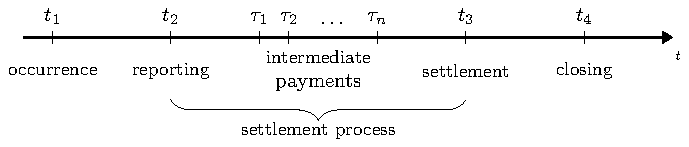
\includegraphics{_main_files/figure-latex/settlement-process-1.pdf}
\caption{\label{fig:settlement-process}Claim timeline.}
\end{figure}

From the moment the claim is reported (\(t_2\)), the insurer estimates how much he is going to pay for that claim and he allocates that sum in a reserve. As new information emerges and some payments are settled, the reserve is updated. The aim for this reserve is to have a best estimate for the future payments for the claims already emerged. As the claim gets settled, the sum between the payed and the reserved converges to the final cost of the claim.

From this description emerges that:

\begin{itemize}
\tightlist
\item
  In the period \(]t_1, t_2[\) the insurer has an outstanding loss liability for an event that has not been reported yet; in this case we will talk about \emph{Incurred But Not Yet Reported} claim (\emph{IBNyR}).
\item
  In the period \([t_2, t_3[\) the insurer has an outstanding loss liability for an event that has been reported, but has not been totally settled yet, so that liability is just an estimate; in this case we will talk about \emph{Incurred But Not Enough Reported} claim (\emph{IBNeR}).
\end{itemize}

\hypertarget{model-fitting-with-available-data}{%
\subsubsection{Model fitting with available data}\label{model-fitting-with-available-data}}

The IBNyR and IBNeR issue is particularly challenging when we have to perform a risk evaluation at a specific time \(t\). In general \(t_1, t_2,\dots\) are not known a priori, so we don't know if in the future more claims for accidents occurred in the past will be reported and we don't know if the ones that are already reported will experience a revaluation. That means that, in general, when we model \(N\) and \(Z\) at a specific time \(t\), we can't observe the total number of claims occurred to each policy \(n_i\) and the payments for each claim \(z_j\). What we can use is:

\begin{itemize}
\tightlist
\item
  \(n_i^{(t)} = n_i^{(\text{reported in } t)}\)\\
  where:

  \begin{itemize}
  \tightlist
  \item
    \(n_i^{(\text{reported in } t)}\) is the number of reported claims in \(t\) for the policy \(i\);
  \end{itemize}
\item
  \(z_j^{(t)} = z_j^{(\text{payed in }t)} + z_j^{(\text{reserved in } t)}\)\\
  where:

  \begin{itemize}
  \tightlist
  \item
    \(z_j^{(\text{payed in }t)}\) is the amount already payed in \(t\) for the claim \(j\);
  \item
    \(z_j^{(\text{reserved in } t)}\) is the amount reserved in \(t\) for the claim \(j\).
  \end{itemize}
\end{itemize}

When we use this data for modeling the total cost of claims we must be particularly aware on what we are using. In general:
\[
n_i^{(t)} \ne n_i, \qquad z_j^{(t)} \ne z_j
\]

The common case is that \(n_i^{(t)} < n_i\) and \(z_j^{(t)} < z_j\). If we used \(n_i^{(t)}\) and \(z_j^{(t)}\) without any correction, we would underestimate both \(E(N)\) and \(E(Z)\), obtaining a biased estimate for \(E(S)\).

To tackle these problems what is usually done is fitting the models for \(S_i\) with \(n_i^{(t)}\) and \(z_j^{(t)}\) and then apply a flat corrective coefficient \(\alpha\) to \(\widehat{E(S_i)}\) based on an aggregated estimate of \(E(S)\) that takes into account the long settlement process.

An estimate for the expected total cost of claims for a generic policy in the portfolio \(E(S)\) can be obtained with techniques based on runoff triangles, such as the \emph{Chain Ladder}. These techniques are based on projecting the cost of claims already emerged to the final total cost of claims. We are not going to discuss these techniques in this thesis. We just have to know that these techniques provide us with an estimate for \(E(S)\). Let's call it \(\widehat{E(S)}^{CL}\). This estimate does not depend on explanatory variables; it is a sort of average total cost of claims for the policies in the portfolio.

Meanwhile, with the available data \(n_i^{(t)}\) and \(z_j^{(t)}\), the fitting for all the models needed in the decomposition of \(S\) is performed and, for each policy \(i\in\{1, 2, \dots, n\}\), \(E(S_i)\) is obtained. Let's call it \(\widehat{E(S_i)}'\). As we used the data available in \(t\) that comes from claims not totally settled, \(\widehat{E(S_i)}'\) is a biased estimate for \(E(S_i)\).

We can then balance the estimates \(\widehat{E(S_i)}'\) with \(\widehat{E(S)}^{CL}\) by computing:
\[
\alpha = \frac{n}{\sum_{i=1}^{n}{\widehat{E(S_i)}'}} \widehat{E(S)}^{CL}
\]
and applying to the estimates as follows:
\[
\widehat{E(S_i)} = \alpha \ \widehat{E(S_i)}'
\]
We will call \(\widehat{E(S_i)}\) rebalanced estimates.

The property of these rebalanced estimates is that on average they are equal to \(\widehat{E(S)}^{CL}\):
\begin{align*}
\frac{\sum_{i=1}^{n}{\widehat{E(S_i)}}}{n} & = \frac{\sum_{i=1}^{n}{\alpha\widehat{E(S_i)}'}}{n} \\
& = \alpha\frac{\sum_{i=1}^{n}{\widehat{E(S_i)}'}}{n} \\
& = \frac{n}{\sum_{i=1}^{n}{\widehat{E(S_i)}'}} \widehat{E(S)}^{CL} \frac{\sum_{i=1}^{n}{\widehat{E(S_i)}'}}{n} \\
& = \widehat{E(S)}^{CL}
\end{align*}

So, if \(\widehat{E(S)}^{CL}\) is a unbiased estimator for \(E(S)\), we obtain:
\[
E\left( \frac{\sum_{i=1}^{n}{\widehat{E(S_i)}}}{n} \right)
= E\left( \widehat{E(S)}^{CL} \right)
= E(S)
\]

This procedure can be further developed by balancing not directly the total cost of claims \(E(S)\), but its components. For example, we could separately balance the total cost of claims that only caused damage to things and the total cost of claims that caused injuries. This separation in components can lead to a more precise estimate because usually claims that caused injuries have a slower settlement process so they will have a higher corrective coefficient \(\alpha\).

If the dataset contains policies from many years and during the last years a relevant change in the portfolio risk mixture happened, it is also possible to compute \(\alpha\) only with the policies from the last year of the dataset, rather than with all the \(n\) policies of the dataset.

The fact that the final estimates \(\widehat{E(S_i)}\) are rebalanced on \(\widehat{E(S)}^{CL}\) means that the explanatory variables effects estimated with \(n_i^{(t)}\) and \(z_j^{(t)}\) are used just as relative effects and not absolute ones. For instance, if the model says that young people have an expected total cost of claims \(\widehat{E(S_i)}'\) that is two times the old people one, that relative coefficient 2 will be kept also in the balanced estimate \(\widehat{E(S_i)}\).

For this reason, in practice, often the modeling is considered composed in 2 parts:

\begin{enumerate}
\def\labelenumi{\arabic{enumi}.}
\tightlist
\item
  \emph{Tariff Requirement} (or \emph{Fabbisogno Tariffario}): the estimate of \(\widehat{E(S)}^{CL}\) by aggregated data;
\item
  \emph{Personalization}: the estimate of \(\widehat{E(S_i)}'\) and the relative coefficients.
\end{enumerate}

The techniques used for \emph{Tariff Requirement} are employed also to estimating the Claim Reserve, that is a fundamental component of the financial statement in Non-Life insurace companies.

\hypertarget{beyond-technical-pricing}{%
\section{Beyond technical pricing}\label{beyond-technical-pricing}}

In section \ref{chap:risk-prem-tech-price} we defined:

\begin{itemize}
\tightlist
\item
  the \emph{Risk Premium}\\
  \(P^{(risk)} = E(S)\)
\item
  the \emph{Technical Price}\\
  \(P^{(tech)} = E(S) + E\)
\end{itemize}

In section \ref{chap:personalization} we described how the risk premium can be estimated. In this thesis we are not going to deal with the estimate of the expenses.

In this section we are going to discuss what the \emph{Tariff} and the \emph{Offer Price} are and which are the further needs that the offer should satisfy. The following description is referred to MTPL insurance in the Italian market. Most of the comments we make can be applied to other motor coverages too.

\hypertarget{tariff-and-offer-price}{%
\subsection{Tariff and Offer Price}\label{tariff-and-offer-price}}

The \emph{Tariff} is the official price for the policy. Over the cost of claims and the expenses, it must include all the loadings for cost of capital and profits. The tariff has a particular importance because it is subjected to strict regulations and it must be approved by the supervisory authority, that in Italy is the IVASS (Istituto per la vigilanza sulle Assicurazioni).

In section \ref{chap:pricing-variables} we described some of the explanatory variables that can be used to build the technical price. For technical pricing there are no constraints because it is used only for internal monitoring and the final price proposed to the client does not directly depends on it. However, some of the variables used for technical pricing can't be used in tariff. In particular, the regulations say that companies can't discriminate clients based on sex, ethnic group, religion or place of birth. Thus, for example, even if from statistical data we see that women usually experience less claims than men, we can't discriminate men by offering them a higher price. Moreover, some variables have constraints on tariff coefficients. For example, in MTPL insurance, the bonus-malus class is strongly regulated. Every company must recognize the bonus-malus class matured by clients (even if they matured them with other companies) and the coefficients of this variable must be monotonically increasing, i.e.~a lower class must correspond to a better tariff. We remind that in the Italian bonus-malus system the lower the class the better the premium. Another tariff constraint is that for some coverage, such as MTPL, the insurer has an obligation to contract. That means that whoever the client is, independently to how risky he is, the company must offer a premium and, if the client accepts, the company must underwrite the insurance contract. In this context, if the company offers an unreasonably high premium, it could fall in an attempt to avoiding the obligation to contract. For this reason, the tariff can't be arbitrarily high and must contemplate a maximum premium. To be sure that all the costraints has been respected, the tariff, before entering in production, must follow a strict approval process.

To make the offer price more flexible and to facilitate business competition, the supervisory authority allows insurance companies to sell policies not at the tariff price, but at the price obtained subtracting from it a discount \(D_i\ge0\). The premium obtained this way is called \emph{Offer Price}.
\[
P^{(\text{offer})}_i = P^{(\text{tariff})}_i - D_i
\]

That means that, for the offer price to adequately cover the cost of claims and expenses, the tariff must include a loading for discounting. This loading for discounting, called \emph{discounting flexibility}, can be partially spent by the agent and partially by the insurance company itself. The discounts can be changed over time in a much more agile way than the tariff. For example in Italy, during the Spring 2020 Covid19 crisis, many companies introduced measures to support customers needs with important discounts on both new business and renewals. From a technical point of view, these discounts have been funded by the remarkable decrese on claim frequency due to the traffic decreasing. Discount measures like these are welcomed by the supervisory authority because they promote business competition and lead to lower prices for consumers.

\hypertarget{price-optimization}{%
\subsection{Price Optimization}\label{price-optimization}}

Both tariff and offer price must be based not only on technical logic, but also on commercial logic. They are determined with a process of \emph{Price Optimization}. The final goal for a company is to maximize profits this year and in the next ones, so the objective of price optimization must be obtaining the optimal price to reach this goal. Maximizing profits is a quite generic goal and can't be easily expressed as an analytical optimization problem. For this reason the pricing choices can be guided by the business strategy that can be translated in specific \emph{Key Performance Indicators} (KPI) that have to be optimized. In this optimization framework, the technical price can be seen as an estimate of the expected cost related to the policy. Knowing the costs it is possible to tune the final premium by working on margins.

The components that act on price optimization can be addressed to:

\begin{enumerate}
\def\labelenumi{\arabic{enumi}.}
\tightlist
\item
  \emph{technical pricing};
\item
  \emph{client expectation};
\item
  \emph{business strategy}.
\end{enumerate}

We already extensively covered technical pricing in previous chapters.

Client expectation is basically the price that the client is willing to pay for the specific product. If the client would pay a premium higher than the technical one, the insurance company has the space for determining an offer price higher than the technical one and gaining margins on that contract. To analyze client expectation, what is usually done is:

\begin{itemize}
\tightlist
\item
  for new business modeling his conversion probability;
\item
  for renewal business modeling his retention probability.
\end{itemize}

For example some guarantees or some options are perceived by the clients as being really worth even if their technical price is not so high. The perception of the client depends also on the competitors pricing and how easy comparing offers from different companies is. In the last years, in the Italian market, the development of aggregators has made much easier for consumers to compare offers from different companies, increasing the competition and the attention on pricing. Anyway, if a company is able to differentiate itself from the others and to make its product be perceived as more valuable, it can sell it at a higher price than other companies. For example this can be achived by improving customer care and customer experience.

If the technical price and the conversion probability functions are given, finding the optimal price for a policy can be expressed as an analytical optimization problem. However, to find the optimal price, one should also take into account that usually policies are not sold alone, but in packages of guarantees. With a wider vision, a business strategy could be selling MTPL policy with almost no margins if it allows to sell other guarantees with higher margins. Moreover, as the aim is not to be profitable this year, but also in the following ones, the company should also consider the \emph{lifetime value} of the client. Indeed, a satisfied client will also stipulate other contracts in the future and can bring to the company other clients from his connections. So, selling a policy with small margins today can lead to high margins tomorrow in other policies.

The business strategy could also contemplate being more aggressive on certain targets of client and less on others. For example, if the company is particularly strong in certain regions, it could make sense for it to push in that region to further increase its market share. Vice versa, in regions where the company doesn't sell much, it could be safer not to push too much and to be more careful. In a risk management framework, this can be also interpreted as introducing a further risk margin for clusters where there isn't enough observed data and the lack of information brings to more uncertainty. An aggressive pricing can also make sense for a young company that is growing and it is not supposed to be profitable from the first years. From a marketing point of view this strategy can increase the brand awareness by the clients and can strengthen the company image.

Anyway, a company can't arbitrarily discount policies because an excess in discounting could cause severe drawbacks on a financial perspective. Therefore, an insurance company must always respect the solvency constraints defined by the supervisory authority to safeguard itself from bankruptcy. The company solvency is essential to protect all the stakeholders, that are both the clients and the investors.

\hypertarget{the-actuary-role}{%
\section{The actuary role}\label{the-actuary-role}}

In this technical pricing and price optimization framework, the actuary is the one that conducts the analysis and defines the pricing rules. The \emph{International Actuarial Association} (IAA) describes the actuaries as ``highly qualified professionals who analyze the financial impact of risk for organizations like insurers, pensions fund managers, and more'' and it states that their work ``requires a combination of strong analytical skills, business knowledge, and understanding of human behavior''.\footnote{\href{https://www.actuaries.org/iaa/IAA/About_the_IAA/About_Actuaries/About\%20Actuaries.aspx}{IAA, About Actuaries}}

First of all, the actuary must master the main statistical and data science techniques used to develop models for technical pricing. On this field, in the last years, the development of machine learning and high performance computing has permitted a huge development of technical pricing allowing actuaries to use much more complex variables and models. However, the actuary does not have just to be an expert in statistics and machine learning. He must be also able to interpret the results he gets with his models and use his expertise to understand if the results he gets are fine for future predictions. As we already mentioned, the pricing rules will be used for policies that will be sold in the future, so they have to be defined with a mixture of observation of the past and assumptions on the future. In addition, sometimes it is needed to define prices for clusters where the company have no historical data. This can happen when a company is expanding to new customers for example by opening new selling channels or by pushing in regions where its market share is quite small. Furthermore, the lack of historical data can be due to the full sector evolution. For example, in these years, new vehicles, such as electric cars and cars with Advanced Driver-Assistance Systems (ADAS), are spreading. As these vehicles didn't exist in the past, historical data doesn't exist. So, finding the proper pricing is challenging. From the company point of view, positioning with a competitive pricing on these segments is important for future business, but the risk must be properly evaluated. For these kind of tasks, the actuary must have a deep domain knowledge on the field.

In the last years, the increase of competition brought to an increase in price optimization importance. Now most of the companies build their own conversion and retention probability models and they are developing more complex business strategies. In this context, it is fundamental for the actuary to understand the clients behaviors, in order to optimize tariff and offer price.

The importance for price optimization implies that the technical pricing must not be conducted independently from tariff and offer pricing. Even in companies where the technical pricing and the offer pricing are carried out by two separate teams, the two teams have to collaborate and coordinate together. This need has some relevant implications on how technical pricing is conducted that we will further discuss in section \ref{chap:actuary-importance}.

--\textgreater{}

\hypertarget{chap:models}{%
\chapter{\texorpdfstring{\textbf{Statistical models for Non Life Insurance Pricing}}{Statistical models for Non Life Insurance Pricing}}\label{chap:models}}

\minitoc  

\chaptermark{Statistical models for Non Life Insurance Pricing}

In this chapter we are going to illustrate some of the most widespread models for technical pricing. For each model we are going to describe its benefits and drawbacks and in section \ref{chap:considerations-on-models} we will compare them by discussing how they fit the pricing needs.

\hypertarget{statistical-models}{%
\section{Statistical Models}\label{statistical-models}}

In this section we will start by describing the Generalized Linear Model (GLM), that is the most employed model in technical pricing, to then present some of its advancements: the Generalized Additive Model (GAM) and the Shrinkage estimators for GLM. After this description, we will also present the Gradient Boosting Machine (GBM), that is one of the most effective general purpose machine learning models. This allows us to have a comparison between GLM based models and general purpose machine learning models.

\hypertarget{glm}{%
\subsection{GLM}\label{glm}}

\hypertarget{chap:linear-exp-families}{%
\subsubsection{Linear Exponential Families}\label{chap:linear-exp-families}}

One of the GLM assumptions is that the response variables belong to a \emph{Linear Exponential Family}. In this section we are going to explain what a linear exponential family is and which distributions fit its definition.

\begin{definition}[Linear Exponential Family]
\label{def:linear-exp-family} \iffalse (Linear Exponential Family) \fi{} A Linear Exponential Family \(\mathcal{F}\) is a parametrical family of probability distributions with density function (or probability function in the discrete case) that can be expressed in the form:
\[
f(y; \theta, \lambda) = \exp{\left\{ \frac{y\theta-b(\theta)}{\lambda} \right\}} c(y,\lambda), \quad y\in \mathcal{Y}\subseteq\mathbb{R}
\]
where:

\begin{itemize}
\item $\theta\in\Theta\subseteq\mathbb{R}$ is called \textit{canonical parameter};
\item $\lambda\in\Lambda\subseteq]0, +\infty[$ is called \textit{dispersion parameter};
\item $b: \Theta \rightarrow \mathbb{R}$ is a real function called \textit{cumulant function};
\item $c: (\mathcal{Y}, \Lambda) \rightarrow [0, +\infty[$ is a real function;
\item $\Theta$ is a non degenerate interval, i.e. $\text{int}\Theta$ is not empty.
\end{itemize}
\end{definition}

An exponential family \(\mathcal{F}\) is characterized by the elements \(\left( \Theta, b(\cdot), \Lambda, c(\cdot, \cdot) \right)\). By properly choosing the sets \(\Theta, \Lambda\) and the functions \(b(\cdot), c(\cdot, \cdot)\), it is possible to obtain many useful families.

It can be easily shown that the families Normal, Poisson, Gamma and Binomial are exponential families. In table \ref{tab:exp-families} the characterizations for these exponential families are reported.

\begin{table}[!h]

\caption{\label{tab:exp-families}Some Linear Exponential Families.}
\centering
\begin{tabular}[t]{lcccccc}
\toprule
\textbf{Distribution} & \textbf{Notation} & \textbf{$\Theta$} & \textbf{$\theta$} & \textbf{$\Lambda$} & \textbf{$\lambda$} & \textbf{$b(\theta)$}\\
\toprule\addlinespace
Normal & \makecell[c]{$N(\mu, \sigma^2)$,\\$\mu\in\mathbb{R}$ \\ $\sigma \in ]0, +\infty[$} & $\mathbb{R}$ & $\mu$ & $]0, +\infty[$ & $\sigma^2$ & $\frac{\theta^2}{2}$\\
\addlinespace\hline\addlinespace
Poisson & \makecell[c]{$Poisson(\mu)$,\\$\mu \in ]0, +\infty[$} & $\mathbb{R}$ & $\log{(\mu)}$ & $\left\{1\right\}$ & $1$ & $e^{\theta}$\\
\addlinespace\hline\addlinespace
Gamma & \makecell[c]{$Gamma(\alpha, \mu)$,\\$\alpha \in ]0, +\infty[$ \\ $\mu \in ]0, +\infty[$} & $]-\infty, 0[$ & $-\frac{1}{\mu}$ & $]0,+\infty[$ & $\frac{1}{\alpha}$ & $-\log{\left(-\theta\right)}$\\
\addlinespace\hline\addlinespace
\makecell[l]{Scaled\\Binomial} & \makecell[c]{$Binom(n, p)/n$,\\$n\in\mathbb{N}$ \\ $p\in]0,1[$} & $\mathbb{R}$ & $\log{\left(\frac{p}{1-p}\right)}$ & $\left\{\frac{1}{n}\right\}$ & $\frac{1}{n}$ & $\log\left(1+e^{\theta}\right)$\\
\bottomrule
\end{tabular}
\end{table}

The distributions that belong to an exponential family have many useful properties. For example they are provided with all the moments and their moments can be obtained using the derivatives of the cumulative function \(b(\cdot)\). If \(Y\) is a random variable with distribution belonging to an exponential family \(\mathcal{F}\) with parameters \(\theta, \lambda\), its first two moments are:
\begin{align}
\label{eq:exp-fam-expected-value}
E(Y)   & = b'(\theta) \\
Var(Y) & = \lambda b''(\theta)
\end{align}

As, within a specified family, the parameters \(\theta\) and \(\lambda\) determine a distribution, in practical problems the object of estimation will be the couple \((\theta, \lambda)\). In many problems it is natural to consider distributions from a linear exponential family where the dispersion parameter can be expressed as \(\lambda = \frac{\phi}{\omega}\), where \(\omega>0\) is a known \emph{weight} and \(\phi>0\) is a parameter that we will keep calling \emph{dispersion parameter}. In this case, the density of probability function depends on the parameters \(\theta\) and \(\phi\) and will be expressed as:
\[
f(y; \theta, \phi, \omega) = \exp{\left\{ \frac{\omega}{\phi} \left[y\theta - b(\theta) \right] \right\}} c(y, \phi, \omega), \quad y\in \mathcal{Y}\subseteq\mathbb{R}
\]

In this case the parameters \(\theta\) and \(\phi\) will be object of estimation, while \(\omega\) is an already known value. As we will see later, this representation allows us to consider as known weights:

\begin{itemize}
\tightlist
\item
  the exposure \(v\) in the Poisson distribution;
\item
  the number of trials \(n\) in the Binomial distribution.
\end{itemize}

\hypertarget{chap:glm-assumptions}{%
\subsubsection{Model assumptions}\label{chap:glm-assumptions}}

Let's assume that, for \(n\) statistical units, the observations \(\mathcal{D} = \left\{ (\boldsymbol{x}_1, \omega_1, y_1), \dots, (\boldsymbol{x}_n, \omega_n, y_n) \right\}\) are available, where \(\boldsymbol{x}_i\) is a vector of explanatory variables determinations, \(\omega_i\) is a known weight and \(y_i\) is the response variable determination. \(\boldsymbol{x}_i, \omega_i, y_i\) are all real numbers. The vector \(\boldsymbol{y} = (y_1, \dots, y_n)^t\) is considered a determination of the response random vector \(\boldsymbol{Y} = (Y_1, \dots, Y_n)^t\).

In GLM we assume that:

\begin{enumerate}
\def\labelenumi{\arabic{enumi}.}
\tightlist
\item
  The response variables \(Y_1, \dots, Y_n\) are stochastically independent and with probability distribution belonging to a same linear exponential family; i.e.~the probability distribution of \(Y_i\) has density function (or probability function in the discrete case) that can be expressed as:
  \[
  f(y_i; \theta_i, \phi, \omega_i) = \exp{\left\{ \frac{\omega_i}{\phi} \left[y_i\theta_i - b(\theta_i) \right] \right\}} c(y_i, \phi, \omega_i), \quad y_i\in \mathcal{Y}\subseteq\mathbb{R}
  \]
  We highlight that only \(\theta_i\) and \(\omega_i\) depend on \(i\), while the dispersion parameter \(\phi\) is the same for all the observations.
\item
  The explanatory variables determinations vector \(\boldsymbol{x}_i = \left(1, x_{i1}, \dots, x_{ip} \right)^t\) affects the probability distribution of the response variable \(Y_i\) by the linear predictor:
  \[
  \eta_i = \beta_0 + \beta_1 x_{i1} + \beta_2 x_{i2} + \dots + \beta_p x_{ip}
  \]
  that is a linear function of the regression parameters \(\boldsymbol{\beta} = \left( \beta_0, \beta_1, \dots, \beta_p \right)\).
\item
  The linear predictor \(\eta_i\) is linked to the expected value of the response variable \(\mu_i = E(Y_i)\) by the following relation:
  \[
  g(\mu_i) = \eta_i = \boldsymbol{x}_i^t \boldsymbol{\beta}
  \]
  where \(g:\mathbb{R}\rightarrow\mathbb{R}\) is a monotonic function with continuous first and second derivatives. \(g(\cdot)\) is called \emph{link function}.
\end{enumerate}

Often, the assumption 1 is called stochastic assumption, while the 2 and 3 are called structural assumptions.

Let's indicate with \(\boldsymbol{X}\) the design matrix, i.e.~the matrix in which each row \(\boldsymbol{x}_{i\cdot}\) represents the vector of the explanatory variables for the observation \(i\) and each column \(\boldsymbol{x}_{\cdot j}\) represents the vector of the observations for the explanatory variable \(j\). The design matrix is represented in figure \ref{fig:design-matrix}. The matrix starts with a column of 1s, that is used to model the intercept. Thus, it is a matrix \(n\times(p+1)\). We assume, as it is common in actuarial datasets, that \(n>p+1\).

\begin{figure}[!hbtp]

{\centering 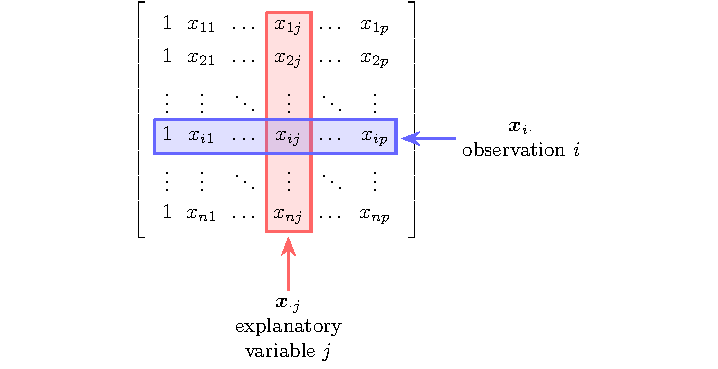
\includegraphics{_main_files/figure-latex/design-matrix-1} 

}

\caption{Design Matrix $\boldsymbol{X}$.}\label{fig:design-matrix}
\end{figure}

We can then express the GLM structural assumptions in a matrix form as:
\[
\boldsymbol{g}(\boldsymbol{\mu}) = \boldsymbol{X} \boldsymbol{\beta}
\]
where \(\boldsymbol{g}(\cdot)\) must be intended as the vectorial function that links every \(\mu_i\) to \(g(\mu_i)\).
\[
\begin{array}{cccc}
\boldsymbol{g}: & \mathbb{R}^n & \longrightarrow & \mathbb{R}^n \\
                & \left(
                    \begin{matrix} \mu_1  \\ \vdots \\ \mu_n \end{matrix}
                  \right)
                  & \longmapsto & 
                  \left(
                    \begin{matrix} g(\mu_1)  \\ \vdots \\ g(\mu_n) \end{matrix}
                  \right)
\end{array}
\]

We assume the design matrix to be a full rank matrix, i.e.~\(\text{rank}(\boldsymbol{X}) = p+1\). This assumption corresponds to assuming that the columns of \(\boldsymbol{X}\) are linearly independent.

The function \(g(\cdot)\) can be chosen as any monotonic function with continuous first and second derivatives. Given a family \(\mathcal{F}\), a common choice is its canonical link function that is defined as:
\[
g(\mu) = b'^{-1}(\mu)
\]
From \eqref{eq:exp-fam-expected-value} we obtain that, as \(\mu = b'(\theta)\), choosing the canonical function corresponds to using \(\theta\) as the linear predictor:
\[
\eta = g(\mu) = b'^{-1}(\mu) = \theta
\]

In table \ref{tab:can-link-fun} the canonical link functions for the families mentioned in \ref{tab:exp-families} are reported.

\begin{table}[!h]

\caption{\label{tab:can-link-fun}Canonical link functions.}
\centering
\begin{tabular}[t]{lccc}
\toprule
\textbf{Distribution} & \textbf{\makecell[c]{Cumulant function\\$b(\theta)$}} & \textbf{\makecell[c]{Derivative\\$b'(\theta)$}} & \textbf{\makecell[c]{Canonical link function\\$g(\mu)=b'^{-1}(\mu)$}}\\
\toprule\addlinespace
Normal & $\frac{\theta^2}{2}$ & $\theta$ & $\mu$\\
\addlinespace\hline\addlinespace
Poisson & $e^{\theta}$ & $e^\theta$ & $\log{(\mu)}$\\
\addlinespace\hline\addlinespace
Gamma & $-\log{\left(-\theta\right)}$ & $-\frac{1}{\theta}$ & $-\frac{1}{\mu}$\\
\addlinespace\hline\addlinespace
\makecell[l]{Scaled\\Binomial} & $\log\left(1+e^{\theta}\right)$ & $\frac{e^{\theta}}{1 + e^{\theta}}$ & $\log{\left( \frac{p}{1-p} \right)}$\\
\bottomrule
\end{tabular}
\end{table}

In the Gamma case, its canonical function \(g(\mu)=-\frac{1}{\mu}\) has the drawback that it links the expected values \(\mu\in]0,+\infty[\) to \(\eta\in]-\infty, 0[\). This would require some constraints on \(\boldsymbol{\beta}\) because \(\eta=\boldsymbol{x}^t\boldsymbol{\beta}\) would have to be \(<0\). For this reason, it is preferred to use \(g(\mu) = \log(\mu)\) that maps \(]0, +\infty[\) to \(\mathbb{R}\).

In the Scaled Binomial case the canonical function \(g(p) = \log{\left(\frac{p}{1-p}\right)}\) is called logit and its inverse \(g^{-1}(\eta) = \frac{e^{\eta}}{1 + e^{\eta}}\) is called logistic. For Scaled Binomial distribution we keep using the notation \(p\) for the expected value as it corresponds to the probability of success \(p\).

\hypertarget{chap:glm-model-fitting}{%
\subsubsection{Model fitting}\label{chap:glm-model-fitting}}

The model depends on the parameters \(\left(\boldsymbol{\beta}, \phi\right)\). Indeed, the parameters \(\theta_i\) can be obtained by \(\boldsymbol{\beta}\) as:
\[
\theta_i = b'^{-1}(\mu_i) = b'^{-1}(g^{-1}(\eta_i)) = b'^{-1}\left(g^{-1}\left(\boldsymbol{x}_i^t\boldsymbol{\beta}\right)\right)
\]

Therefore, fitting the model corresponds to estimating \(\left(\boldsymbol{\beta}, \phi\right)\). The technique used in GLM is the \emph{Maximum Likelihood}. Let's indicate with \(L\left(\boldsymbol{\beta}, \phi; \boldsymbol{y}\right)\) the model likelihood. We remind that the likelihood is a function of the parameters that maps \(\left(\boldsymbol{\beta}, \phi\right)\) to the density (or probability in the discrete case) of the observed values \(\boldsymbol{y}\) conditioned to the parameters \(\left(\boldsymbol{\beta}, \phi\right)\)
\[
\begin{array}{cccc}
L: & \mathbb{R}^{p+1} \times \Lambda & \longrightarrow & [0, +\infty[ \\
   & \left(\boldsymbol{\beta}, \phi\right) & \longmapsto & f_{\boldsymbol{Y}}(\boldsymbol{y}; \boldsymbol{\theta}, \phi)
\end{array}
\]

The maximum likelihood estimates are the values \(\left(\boldsymbol{\beta}, \phi\right)\) that maximize \(L\left(\boldsymbol{\beta}, \phi; \boldsymbol{y}\right)\). In practice, \(\boldsymbol{\beta}\) are the parameters of interest, while \(\phi\) is considered as a disturbance parameter. It is possible to show that conditioned to any \(\phi\), the value for \(\boldsymbol{\beta}\) that maximizes \(L(\cdot, \cdot)\) does not depend on \(\phi\). Therefore, \(\boldsymbol{\beta}\) and \(\phi\) can be estimated separately.

Let's indicate with \(\tilde{\boldsymbol{\beta}}\) the maximum likelihood estimator for \(\boldsymbol{\beta}\). Its determination \(\hat{\boldsymbol{\beta}}\) is defined as:
\begin{equation}
\label{eq:max-lik-est}
\hat{\boldsymbol{\beta}} = \argmax_{\boldsymbol{\beta}\in\mathbb{R}^{p+1}}{L\left(\boldsymbol{\beta}, \phi; \boldsymbol{y}\right)}
\end{equation}

Finding the values \(\hat{\boldsymbol{\beta}}\) that maximize the likelihood corresponds to finding the values that maximize the log-likelihood \(\ell\left(\boldsymbol{\beta}, \phi; \boldsymbol{y}\right) = \log{\left(L\left(\boldsymbol{\beta}, \phi; \boldsymbol{y}\right)\right)}\). For the independence hypothesis on \(Y_1, \dots, Y_n\) we get:
\begin{align}
\nonumber
\ell\left(\boldsymbol{\beta}, \phi; \boldsymbol{y}\right) & =
\log{\left(L\left(\boldsymbol{\beta}, \phi; \boldsymbol{y}\right)\right)}
\\ \nonumber & =
\log{\left(\prod_{i=1}^{n}{\exp{\left\{ \frac{\omega_i}{\phi} \left[y_i\theta_i - b(\theta_i) \right] \right\}} c(y_i, \phi, \omega_i)}\right)}
\\ \label{eq:log-like} & =
\sum_{i=1}^{n}{
\left\{
\frac{\omega_i}{\phi} \left[y_i\theta_i - b(\theta_i) \right] + \log{\left(c(y_i, \phi, \omega_i)\right)}
\right\}
}
\\ \nonumber & =
\sum_{i=1}^{n}{\ell_i\left(\boldsymbol{\beta}, \phi; \boldsymbol{y}\right)}
\end{align}

The maximum value of \(\ell\left(\boldsymbol{\beta}, \phi; \boldsymbol{y}\right)\) can be obtained by imposing all its partial derivatives equal to \(0\):
\[
\frac{\partial \ell\left(\boldsymbol{\beta}, \phi; \boldsymbol{y}\right)}
{\partial\beta_j}
= 0, \quad \forall j\in\{0,1,\dots,p\}
\]

These equations can be solved with numerical methods, such as Newton-Raphson algorithm or its variant Fisher scoring. It is possible to show that Newton-Raphson algorithm corresponds to iteratively solving a weighted least squares optimization problem.

In the case with Normal response and identity link, the optimization problem \eqref{eq:max-lik-est} has an explicit solution:
\[
\hat{\boldsymbol{\beta}} = \left( \boldsymbol{X}^t \boldsymbol{X} \right)^{-1} \boldsymbol{X}^t \boldsymbol{y}
\]

A statistic that can be used to measure the goodness of fit of a model is the \emph{Deviance}. It can be used by comparing the current model log-likelihood \(\ell\left(\hat{\boldsymbol{\beta}}, \phi; \boldsymbol{y}\right)\) with the \emph{saturated model} log-likelihood \(\ell_{S}\left(\boldsymbol{\beta}^*, \phi; \boldsymbol{y}\right)\). The saturated model is the model with \(n\) parameters, so a model where the expected values of the response variables \(\mu_1, \dots, \mu_n\) are estimated with their observed values \(y_1, \dots, y_n\). It is possible to show that \(\ell_{S}\left(\boldsymbol{\beta}^*, \phi; \boldsymbol{y}\right) \ge \ell\left(\hat{\boldsymbol{\beta}}, \phi; \boldsymbol{y}\right)\). The closer \(\ell\left(\hat{\boldsymbol{\beta}}, \phi; \boldsymbol{y}\right)\) is to \(\ell_{S}\left(\boldsymbol{\beta}^*, \phi; \boldsymbol{y}\right)\), the better the current model fitting is.

\begin{definition}[Deviance]
\label{def:deviance-def} \iffalse (Deviance) \fi{} Given \(\ell\left(\hat{\boldsymbol{\beta}}, \phi; \boldsymbol{y}\right)\) the log-likelihood of the current model and \(\ell_{S}\left(\boldsymbol{\beta}^*, \phi; \boldsymbol{y}\right)\) the log-likelihood of the saturated model, the \textit{Scaled Deviance} of the current model is defined as:
\[
S(\hat{\boldsymbol{\beta}}, \phi, \boldsymbol{y}) =
-2\left(
\ell\left(\hat{\boldsymbol{\beta}}, \phi; \boldsymbol{y}\right)
- \ell_{S}\left(\boldsymbol{\beta}^*, \phi; \boldsymbol{y}\right)
\right)
\]
The \textit{Deviance} of the current model is defined as:
\[
D(\hat{\boldsymbol{\beta}}, \boldsymbol{y}) =
\phi \, S(\hat{\boldsymbol{\beta}}, \phi, \boldsymbol{y})
\]
\end{definition}

In deviance notation \(D(\hat{\boldsymbol{\beta}}, \boldsymbol{y})\), the parameter \(\phi\) is not reported because the deviance does not depend on \(\phi\). Indeed, from \eqref{eq:log-like} we get:
\begin{align*}
S(\hat{\boldsymbol{\beta}}, \phi, \boldsymbol{y})
& =
-2\left(
\ell\left(\hat{\boldsymbol{\beta}}, \phi; \boldsymbol{y}\right)
- \ell_{S}\left(\boldsymbol{\beta}^*, \phi; \boldsymbol{y}\right)
\right)
\\ & =
-2\left(
\sum_{i=1}^{n}{
\left\{
\frac{\omega_i}{\phi} \left[y_i\hat{\theta}_i - b(\hat{\theta}_i) \right] + \log{\left(c(y_i, \phi, \omega_i)\right)}
\right\}
}
\right.
\\ & \qquad \qquad -
\left.
\sum_{i=1}^{n}{
\left\{
\frac{\omega_i}{\phi} \left[y_i\theta_i^* - b(\theta_i^*) \right] + \log{\left(c(y_i, \phi, \omega_i)\right)}
\right\}
}
\right)
\\ & =
-2\left(
\sum_{i=1}^{n}{
\frac{\omega_i}{\phi}
\left\{
\left[y_i\hat{\theta}_i - b(\hat{\theta}_i) \right]
- \left[y_i\theta_i^* - b(\theta_i^*) \right]
\right\}
}
\right)
%
\\[12pt]
%
D(\hat{\boldsymbol{\beta}}, \boldsymbol{y})
& =
-2\left(
\sum_{i=1}^{n}{
\omega_i
\left\{
\left[y_i\hat{\theta}_i - b(\hat{\theta}_i) \right]
- \left[y_i\theta_i^* - b(\theta_i^*) \right]
\right\}
}
\right)
\end{align*}

In table \ref{tab:deviance} the deviances for the families mentioned in \ref{tab:exp-families} are reported.

\begin{table}[!h]

\caption{\label{tab:deviance}Deviance for Linear Exponential Families}
\centering
\begin{tabular}[t]{lc}
\toprule
\textbf{Distribution} & \textbf{Deviance $D(\hat{\boldsymbol{\beta}}, \boldsymbol{y})$}\\
\toprule\addlinespace
Normal & $\sum_{i=1}^{n}{\left( y_i - \hat{\mu}_i \right)^2}$\\
\addlinespace\hline\addlinespace
Poisson & $2\,\sum_{i=1}^{n}{\left\{ y_i \log{\left(\frac{y_i}{\hat{\mu}_i}\right)} - \left( y_i - \hat{\mu}_i \right) \right\}}$\\
\addlinespace\hline\addlinespace
Gamma & $2\,\sum_{i=1}^{n}{\left\{ - \log{\left(\frac{y_i}{\hat{\mu}_i}\right)} + \frac{ y_i - \hat{\mu}_i }{\hat{\mu}_i} \right\}}$\\
\addlinespace\hline\addlinespace
\makecell[l]{Scaled\\Binomial} & $2\,\sum_{i=1}^{n}{\left\{ y_i \log{\left(\frac{y_i}{\hat{\mu}_i}\right)}+ \left(1-y_i\right) \log{\left(\frac{1-y_i}{1-\hat{\mu}_i}\right)} \right\}}$\\
\bottomrule
\end{tabular}
\end{table}

As \(\ell_{S}\left(\boldsymbol{\beta}^*, \phi; \boldsymbol{y}\right)\) does not depend on \(\hat{\boldsymbol{\beta}}\), maximizing the likelihood in equation \eqref{eq:max-lik-est} is the same as minimizing the deviance, that can be seen as a \emph{Loss Function}:
\begin{equation}
\label{eq:max-lik-est-deviance}
\hat{\boldsymbol{\beta}} = \argmin_{\boldsymbol{\beta}\in\mathbb{R}^{p+1}}{D(\boldsymbol{\beta}, \boldsymbol{y})}
\end{equation}

\hypertarget{chap:var-effects}{%
\subsubsection{Variable effects}\label{chap:var-effects}}

As we mentioned in \ref{chap:pricing-variables-encoding}, the explanatory variables can be \emph{quantitative} or \emph{qualitative}. In GLM, if explanatory variables transformation terms aren't added to the linear predictor \(\eta\), the variables effect on \(\eta\) is linear. In figure \ref{fig:expl-var-types} the effects of quantitative and qualitative variables are shown. The data is simulated from a GLM with Normal response and identity link.





\begin{figure}[!hbtp]

{\centering \subfloat[Quantitative\label{fig:expl-var-types-1}]{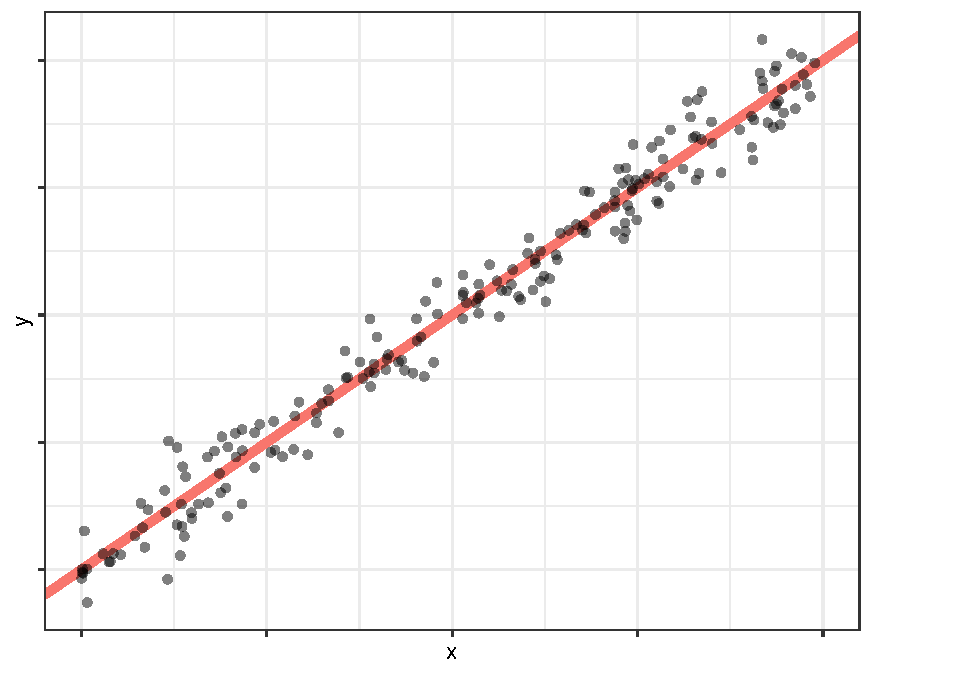
\includegraphics[width=0.5\linewidth]{_main_files/figure-latex/expl-var-types-1} }\subfloat[Qualitative\label{fig:expl-var-types-2}]{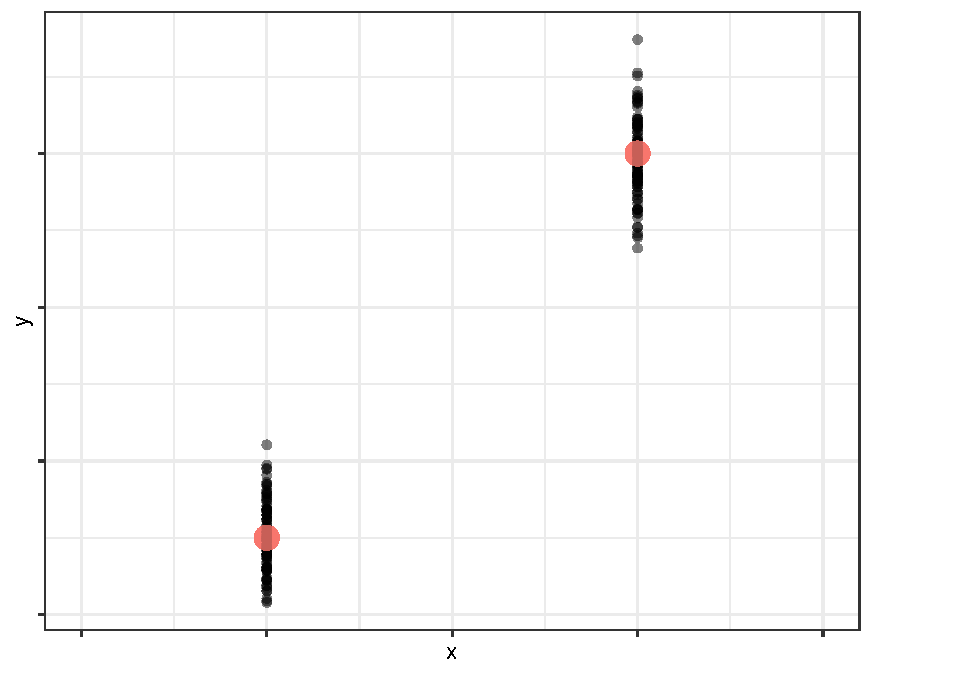
\includegraphics[width=0.5\linewidth]{_main_files/figure-latex/expl-var-types-2} }\newline\subfloat[Quantitative and qualitative \\ without interaction\label{fig:expl-var-types-3}]{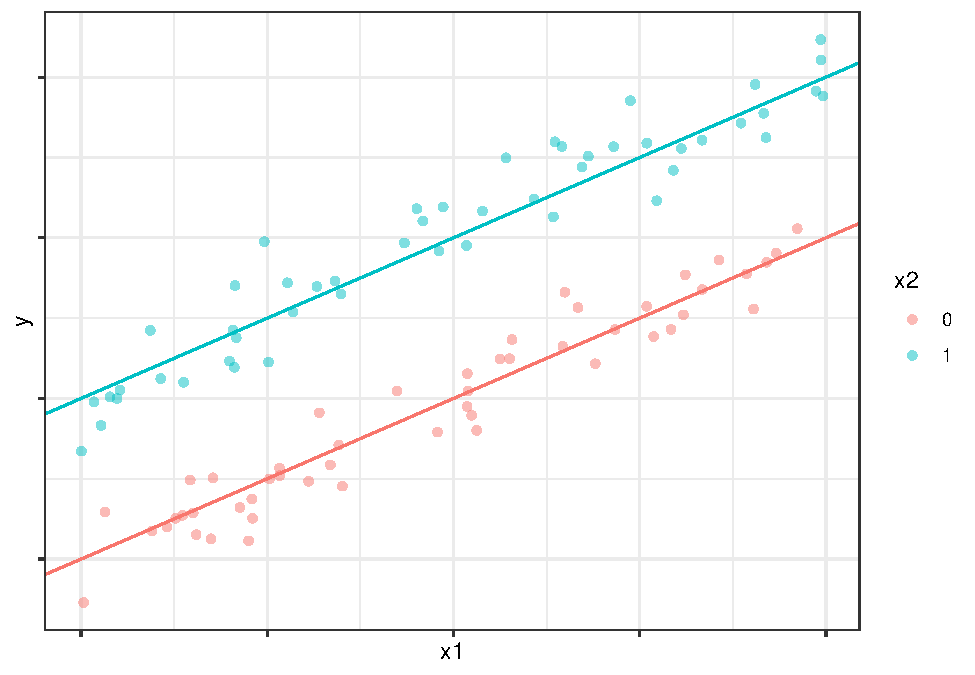
\includegraphics[width=0.5\linewidth]{_main_files/figure-latex/expl-var-types-3} }\subfloat[Quantitative and qualitative \\ with interaction\label{fig:expl-var-types-4}]{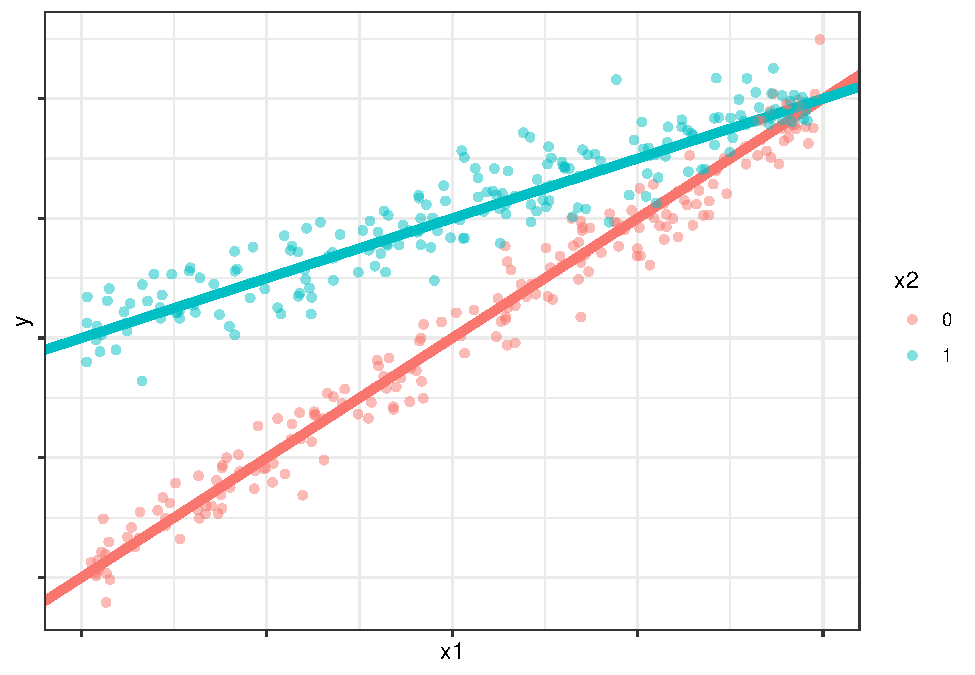
\includegraphics[width=0.5\linewidth]{_main_files/figure-latex/expl-var-types-4} }

}

\caption{Explanatory variables types.}\label{fig:expl-var-types}
\end{figure}

In the top-left panel, we see the effect of the quantitative variable \(x\) in the model \(\mu_i = \beta_0 + \beta_1 x_i\). As we can see it is a straight line. The coefficient \(\beta_1\) represents the slope of the line, thus \(\beta_1>0\) means that \(x\) and \(Y\) are positively correlated, while \(\beta_1<0\) means that \(x\) and \(Y\) are negatively correlated. For example, if \(x\) is the power of the vehicle and \(Y\) the yearly number of claims, \(\beta_1>0\) means that the more powerful the vehicle is, the more claims the policyholder will experience on average.

In the top-right panel, we see the effect of a qualitative binary variable \(x\) in the model \(\mu_i = \beta_0 + \beta_1 x_i\). The variable is encoded with values \(0\) and \(1\), so \(\beta_1\) represents the effect of the modality \(x=1\). In general, for a qualitative variable with \(K\) modalities we will have \(K-1\) dummy variables \(x'_1, \dots, x'_{K-1}\) and the model will be \(\mu_i = \beta_0 + \beta_1 x'_{i1} + \beta_2 x'_{i2} + \dots + + \beta_{K-1} x'_{i, K-1}\). Thus, the \(\beta_j\) coefficient represents the relative effect of the modality \(j\) compared to the base level modality, that is the one not explicitly included in the dummy encoding. For example, if \(x\) is the vehicle make, \(Y\) the yearly number of claims, the base level for \(x\) is `Fiat' and the \(j\)\textsuperscript{th} modality is `Ferrari', then \(\beta_j>0\) means that Ferrari cars on average experience more claims that Fiat cars.

In general, in a multivariate model, the coefficient \(\beta_j\) represents the effect of the variable \(j\) given all the others. In the example of Fiat and Ferrari cars, if in the model there is also the variable `vehicle power', the coefficient \(\beta_j\) corresponding to the modality `Ferrari' represents the how more risky a Ferrari car is compared to a Fiat car with the same power. If the explanatory variables are strongly correlated, it is important to be aware of this aspect. For example, Ferrari cars are usually more powerful that Fiat cars. So, it is possible that in general Ferrari cars are more risky than Fiat cars, but comparing a Ferrari car to a Fiat with the same power, the Ferrari could be less risky. This effect is called \emph{Simpson's paradox} \footnote{Simpson's paradox, \url{https://en.wikipedia.org/wiki/Simpson\%27s_paradox}}.

In the bottom-left panel of figure \ref{fig:expl-var-types}, we see the effect of a quantitative variable \(x_1\) and a qualitative binary variable \(x_2\) together in the model \(\mu_i = \beta_0 + \beta_1 x_{i1} + \beta_2 x_{i2}\). As we can seen, the effects of \(x_1\) variable in the two groups defined by \(x_2\) variable are represented by two parallel straight lines. The first one is \(\mu_i = \beta_0 + \beta_1 x_{i1}\) and the second is \(\mu_i = \left(\beta_0 + \beta_2\right) + \beta_1 x_{i1}\). The coefficient \(\beta_2\) represents the vertical distance between the two lines.

In the bottom-right panel, the interaction effect between \(x_1\) and \(x_2\) is included in the model. The model becomes \(\mu_i = \beta_0 + \beta_1 x_{i1} + \beta_2 x_{i2} + \beta_3 x_{i1} x_{i2}\). That means that the effect of \(x_1\) variables depends on the determination of the \(x_2\) variable. In the group with \(x_2=0\) the effect is represented by the line \(\mu_i = \beta_0 + \beta_1 x_i\); the group with \(x_2=1\) the effect is represented by the line \(\mu_i = \left(\beta_0 + \beta_2\right) + \left(\beta_1 + \beta_3\right) x_{i1}\).

For quantitative variables, it is possible to consider also non linear effects in GLMs. Some examples are reported in figure \ref{fig:expl-var-quant-effect}.





\begin{figure}[!hbtp]

{\centering \subfloat[Polynomial degree 2\label{fig:expl-var-quant-effect-1}]{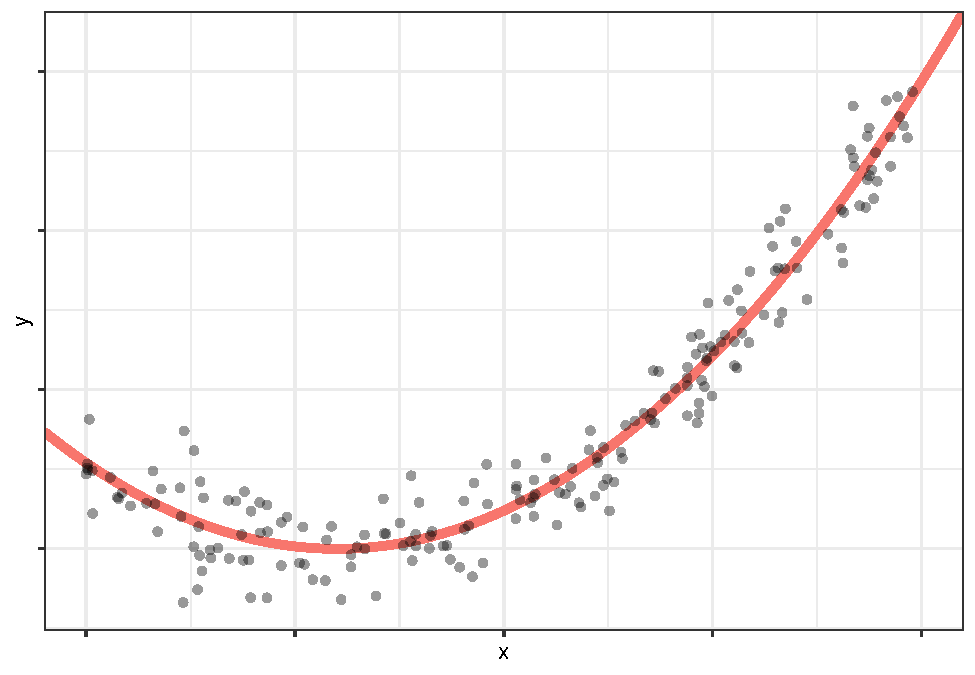
\includegraphics[width=0.5\linewidth]{_main_files/figure-latex/expl-var-quant-effect-1} }\subfloat[Polynomial degree 4\label{fig:expl-var-quant-effect-2}]{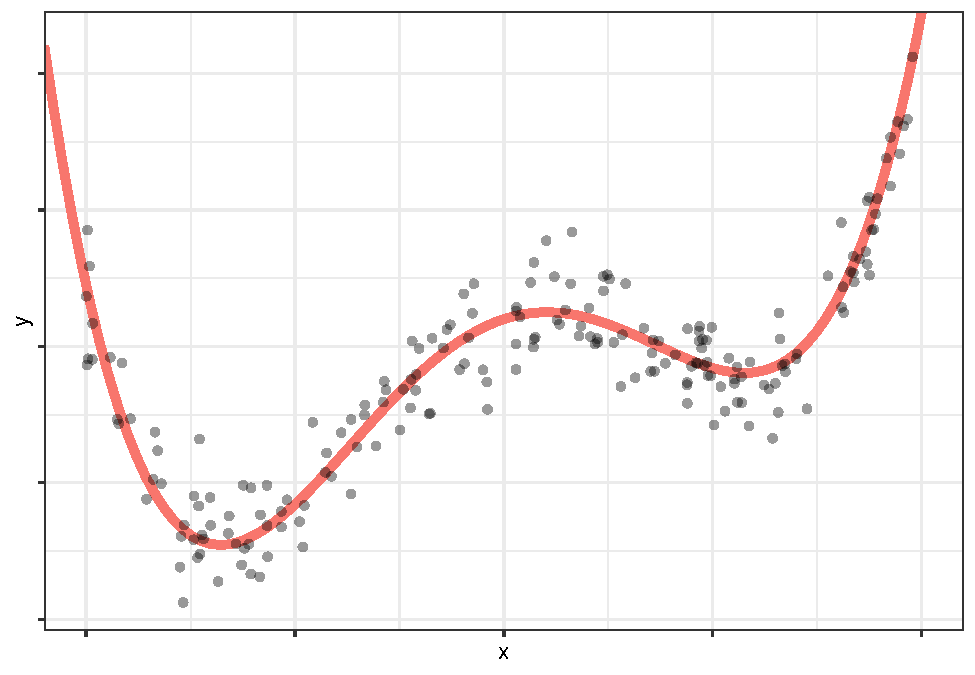
\includegraphics[width=0.5\linewidth]{_main_files/figure-latex/expl-var-quant-effect-2} }\newline\subfloat[Piece-wise linear\label{fig:expl-var-quant-effect-3}]{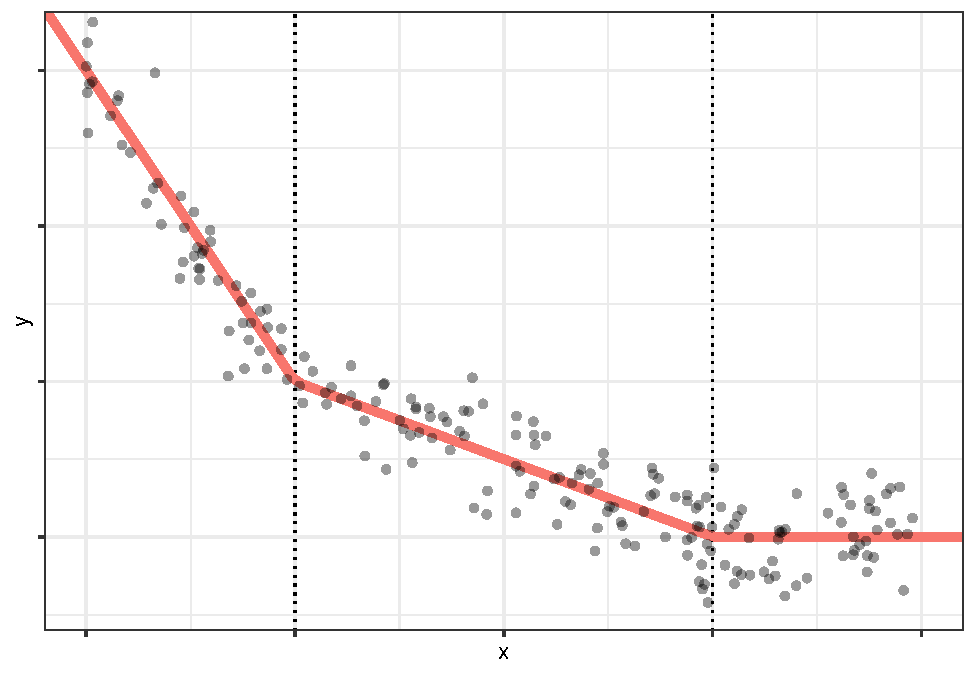
\includegraphics[width=0.5\linewidth]{_main_files/figure-latex/expl-var-quant-effect-3} }\subfloat[Piece-wise polynomial degree 2\label{fig:expl-var-quant-effect-4}]{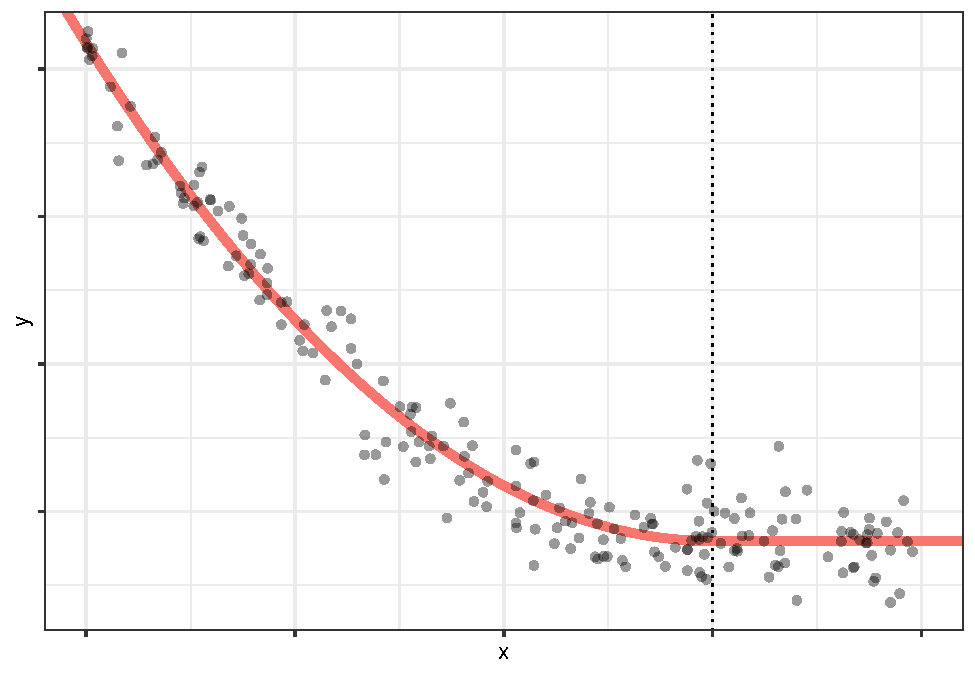
\includegraphics[width=0.5\linewidth]{_main_files/figure-latex/expl-var-quant-effect-4} }

}

\caption{Explanatory quantitative variables effects.}\label{fig:expl-var-quant-effect}
\end{figure}

The basic way to achieve it is by adding polynomial terms to the linear predictor. For instance, if \(x\) is a quantitative variable, it is possible to add to the model the term \(x^2\), obtaining the model \(\mu_i = \beta_0 + \beta_1 x_{i} + \beta_2 x_i^2\). An example of model with both \(x\) and \(x^2\) terms is represented in top-left panel of figure \ref{fig:expl-var-quant-effect}. Adding the quadratic term, the effect graph becomes a parabola.

With the same logic, it is possible to add more power terms. In general, if we want to model \(x\) with a polynomial of degree \(d\), we can consider the model \(\mu_i = \beta_0 + \beta_1 x_{i} + \beta_2 x_{i}^2 + \dots + \beta_d x_{i}^d\). In top-right panel of figure \ref{fig:expl-var-quant-effect} a 4\textsuperscript{th} degree polynomial effect is represented. We highlight that the model is still considered linear, as the attribute ``Linear'' in ``General Linear Model'' is referred to the relation between the parameters \(\beta_j\) and the linear predictor \(\eta_i\) that is still linear.

Another way to model non liner effects of explanatory variables is to separate the effects by pieces. In bottom-left panel of figure \ref{fig:expl-var-quant-effect} a case in which the \(x\) effect is separated in 3 pieces is represented. As in all the pieces the effect is linear, the graph of the variable effect is a broken line. This effect can be achieved by adding to the model the terms \((x-\nu)_+\), where \((x)_+\) represents the positive part of \(x\) (\((x)_+ = \max(0,x)\)) and \(\nu\) is the value of \(x\) in the angular point. The \(\nu\) values are called \emph{knots}, If the knots are \(\nu_1, \nu_2, \dots, \nu_m\), the model can be represented as \(\mu_i = \beta_0 + \beta_1 x_i + \beta_2 (x_i-\nu_1)_+ + \beta_3 (x_i-\nu_2)_+ + \dots + \beta_{m+1} (x_i-\nu_m)_+\). This kind of functions are called \emph{linear splines} and will be further discussed in section \ref{chap:gam}. If we want the effect to be null from a certain point \(\nu\), we can consider the variable \(x' = \min(\nu, x)\) instead of \(x\). This corresponds to aggregate to \(\nu\) all the \(x\) after \(\nu\).

The piece-wise approach can be enhanced by also considering polynomial terms. For instance, in bottom-left panel of figure \ref{fig:expl-var-quant-effect}, the model represented is \(\mu_i = \beta_0 + \left( x_i - \nu \right)_-^2\), where \((x)_-\) is the negative part of \(x\) (\((x)_- = \min(0,x)\)). \(f(x) = (x-\nu)^2\) is a parabola with vertex in \(\nu\). The fact of not adding the linear term leads to a monotonic effect made by a semi-parabola and a horizontal semi-line that starts from its vertex.

The examples represented in figures \ref{fig:expl-var-types} and \ref{fig:expl-var-quant-effect} are based on simulated data. That means that the linear predictor structure is known and the coefficients \(\beta_0, \beta_1, \dots, \beta_J\) are known. In practice, the real model is not known and the coefficients and the structure must be estimated by the data. Thus, we can take assumptions on the structure and we can estimate the coefficients with \(\hat{\beta}_0, \hat{\beta}_1, \dots, \hat{\beta}_J\). In many cases it is not so clear whether to consider or not a variable and how to consider it. For example, with the same data both bottom-left and bottom-right models could work fine. In section \ref{chap:variable-selection} we are going to discuss some variable selection techniques for GLM.

\hypertarget{link-functions-and-relativities}{%
\subsubsection{Link functions and relativities}\label{link-functions-and-relativities}}

As we mentioned in \ref{chap:linear-exp-families}, GLM supports several families. In figure \ref{fig:resp-var} the models \(g(\mu_i) = \beta_0 + \beta_1 x_i\) with different response variable distributions and link functions are represented. As we can see from the plots, a linear effect on \(x\) corresponds to a logistic effect when the link is logit and to an exponential effect when the link is log.





\begin{figure}[!hbtp]

{\centering \subfloat[Normal - identity\label{fig:resp-var-1}]{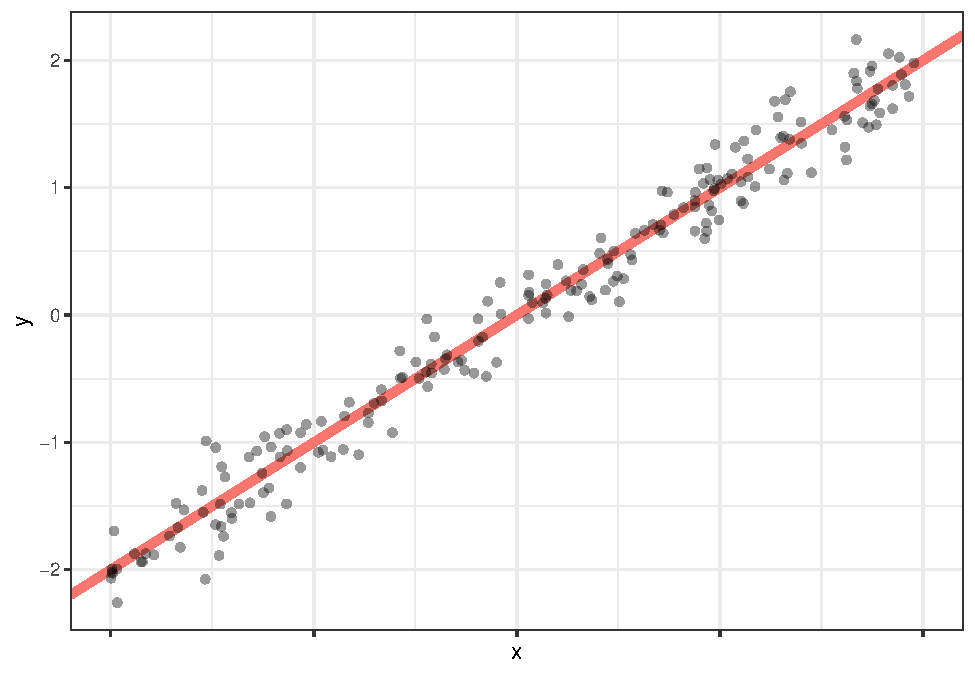
\includegraphics[width=0.5\linewidth]{_main_files/figure-latex/resp-var-1} }\subfloat[Binomial - logit\label{fig:resp-var-2}]{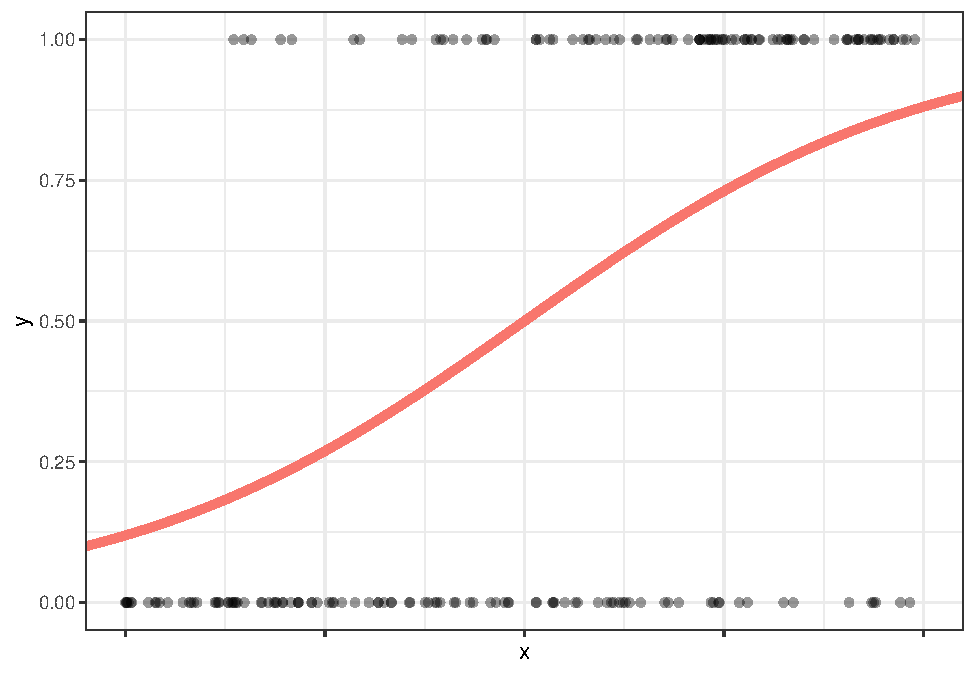
\includegraphics[width=0.5\linewidth]{_main_files/figure-latex/resp-var-2} }\newline\subfloat[Poisson - log\label{fig:resp-var-3}]{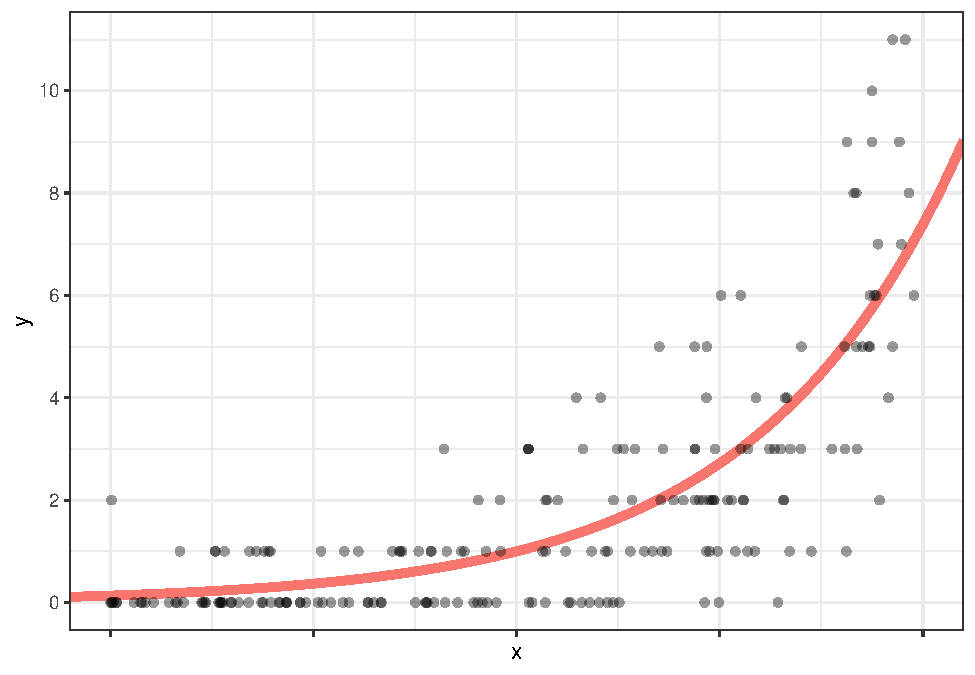
\includegraphics[width=0.5\linewidth]{_main_files/figure-latex/resp-var-3} }\subfloat[Gamma - log\label{fig:resp-var-4}]{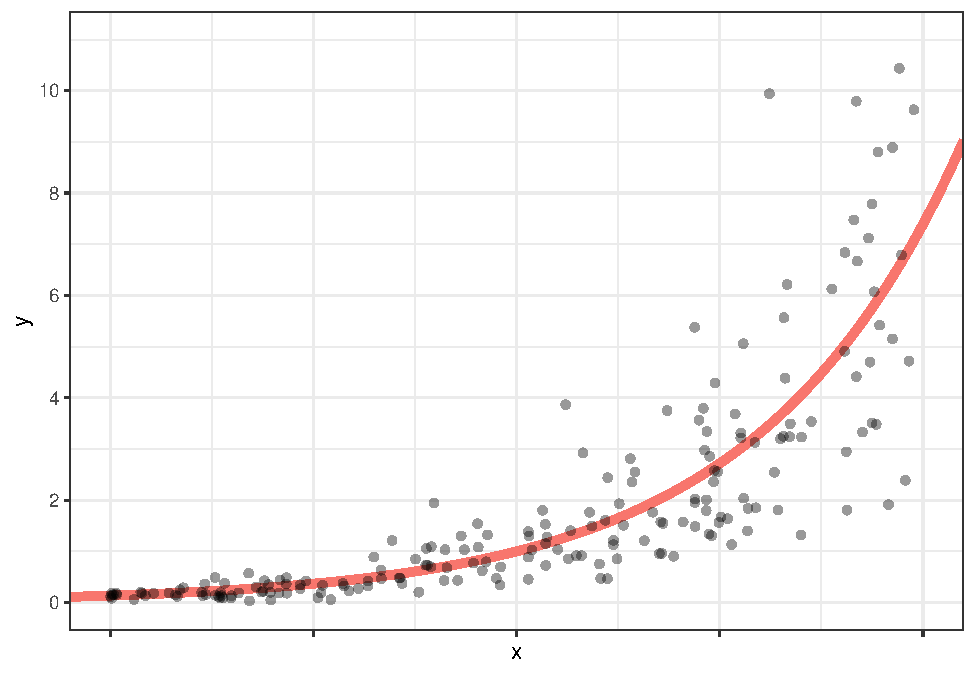
\includegraphics[width=0.5\linewidth]{_main_files/figure-latex/resp-var-4} }

}

\caption{Response variables and link functions.}\label{fig:resp-var}
\end{figure}

If \(g(\mu) = \log(\mu)\), the model structure can be expressed as:
\begin{align*}
\mu_i & = e^{\beta_0 + \beta_1 x_{i1} + \beta_2 x_{i2} + \dots + \beta_p x_{ip}} \\
& = e^{\beta_0} \left(e^{\beta_1}\right)^{x_{i1}} \left(e^{\beta_2}\right)^{x_{i2}} \dots \left(e^{\beta_p}\right)^{x_{ip}}
\end{align*}

The term \(e^{\beta_j}\) can be seen as the multiplicative factor corresponding to the variable \(x_j\). If \(x_j\) is a dummy variable, \(e^{\beta_j}\) is the factor the expected value \(\mu_i\) is multiplied by when \(x_{ij}=1\). If \(x_j\) is a quantitative variable, \(e^{\beta_j}\) is the factor the expected value \(\mu_i\) is multiplied by for every one-unit increasing of \(x_{ij}\). Indeed:
\[\left(e^{\beta_j}\right)^{x_j+1} = e^{\beta_j} \left(e^{\beta_j}\right)^{x_j}\]

The fact that with a log link the relation between coefficients \(\beta_0, \beta_1, \dots, \beta_p\) and expected value \(\mu_i\) becomes multiplicative is particularly useful to deal with exposure \(v_i\). In section \ref{chap:exposure} we have seen that often the observations are couples (policy, accounting year), so they have different exposures \(v_i\). Thus, we usually work with the number of claims occurred in the exposure period \(M_i\) and we observe its realization \(m_i\). The assumption we take is that:
\[M_i \sim Poisson(v_i \mu_i)\]
where \(\mu_i\) is the expected value of the yearly number of claims \(N_i\).

Under the GLM assumptions, we obtain
\begin{align*}
E(M_i) & = v_i \mu_i = v_i e^{\beta_0 + \beta_1 x_{i1} + \dots + \beta_p x_{ip}} \\
& = e^{\log(v_i)}e^{\beta_0 + \beta_1 x_{i1} + \dots + \beta_p x_{ip}} \\
& = e^{\beta_0 + \beta_1 x_{i1} + \dots + \beta_p x_{ip} + \log(v_i)}
\end{align*}

That means that we can model \(M_1, M_2, \dots, M_n\) as response variables in a GLM with Poisson response in which the linear predictor depends on an offset additive term \(\log(v_i)\).

If \(g(p) = \text{logit}(p)\), the model structure can be expressed as:
\begin{align*}
\frac{p_i}{1-p_i} & = e^{\beta_0 + \beta_1 x_{i1} + \beta_2 x_{i2} + \dots + \beta_p x_{ip}} \\
& = e^{\beta_0} \left(e^{\beta_1}\right)^{x_{i1}} \left(e^{\beta_2}\right)^{x_{i2}} \dots \left(e^{\beta_p}\right)^{x_{ip}}
\end{align*}

Thus, the term \(e^{\beta_j}\) can be seen as the multiplicative relativity corresponding to the variable \(x_j\). However, in this case the relativity doesn't multiply directly the probability of success \(p\), but it multiplies the odds of success \(\frac{p}{1-p}\).

\hypertarget{chap:variable-selection}{%
\subsubsection{Variable selection}\label{chap:variable-selection}}

One of the most challenging aspects of GLM fitting is selecting the variables and their effects by looking to observed data. In practice, we usually have many explanatory variables available but only some of them are relevant for the prediction of the response variable. Adding useless variables to the model increases the variance of the estimators of the coefficients \(\tilde{\beta}_0, \tilde{\beta}_1, \dots, \tilde{\beta}_p\) and then the variance of the predictions \(\tilde{\mu}_i = \tilde{\beta}_0 + \tilde{\beta}_1 x_{i1} + \dots + \tilde{\beta}_p x_{ip}\). On the other hand, being too frugal with explanatory variables could lead to wasting part of the predictive power of the available explanatory variables.

One useful tool we have to understand if an explanatory variable \(x\) is relevant or not is plotting the points \((x_i, y_i)\), as we did in \ref{fig:expl-var-types}, \ref{fig:expl-var-quant-effect} and \ref{fig:resp-var}. If there are too many observations and the plot is not easily readable, it is possible to group the points by \(x\) modalities and show for each group the average of \(y_i\) and a confidence interval that gives an idea on the dispersion of the observations around the average. If \(x\) is a continuous variable with too many modalities, it is possible to group them into buckets. Showing the average of \(y_i\) for groups of \(x\) is particularly useful for Binomial and Poisson data, where the fact that \(y_i\) can present few different values compromises the plot readability. An example is reported in figure \ref{fig:var-selection}. The top-left and bottom-left panels represent a case in which \(x\) and \(y\) are not related, while the top-right and bottom-right panels represent a case of positive correlation. From the ungrouped plot in the top-right panel the effect is not clear, while from bottom-right panel it is evident.







\begin{figure}[!hbtp]

{\centering \subfloat[No effect - ungrouped\label{fig:var-selection-1}]{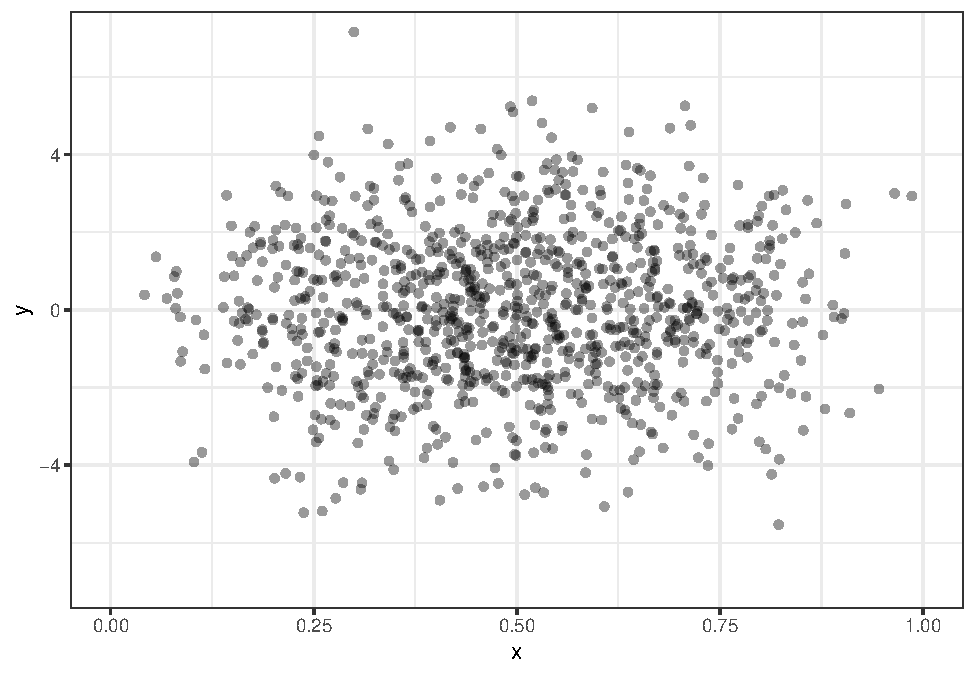
\includegraphics[width=0.5\linewidth]{_main_files/figure-latex/var-selection-1} }\subfloat[Positive effect - ungrouped\label{fig:var-selection-2}]{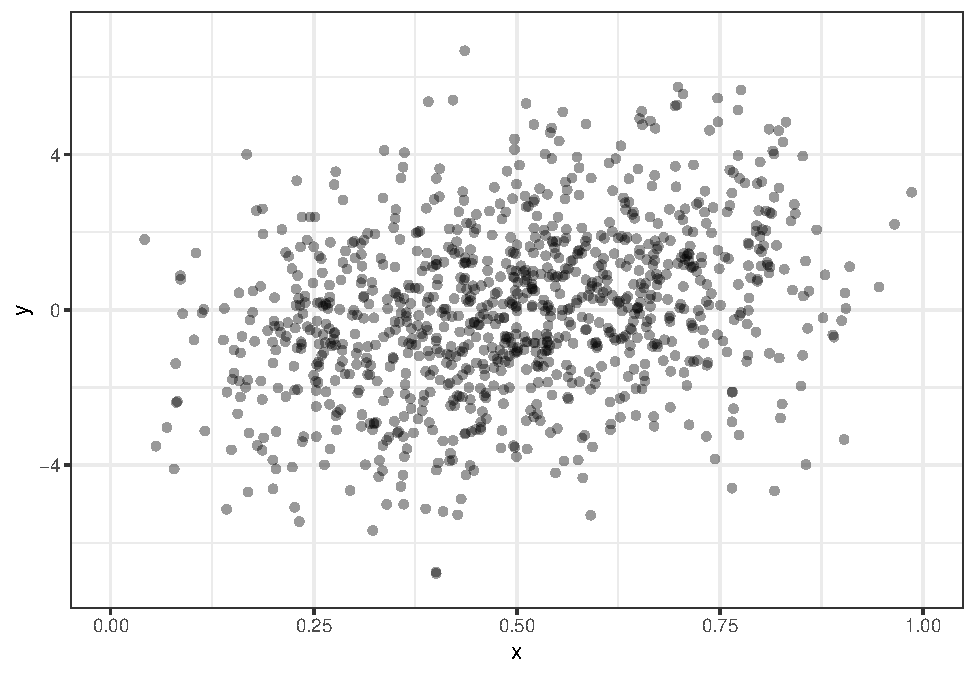
\includegraphics[width=0.5\linewidth]{_main_files/figure-latex/var-selection-2} }\newline\subfloat[No effect - grouped\label{fig:var-selection-3}]{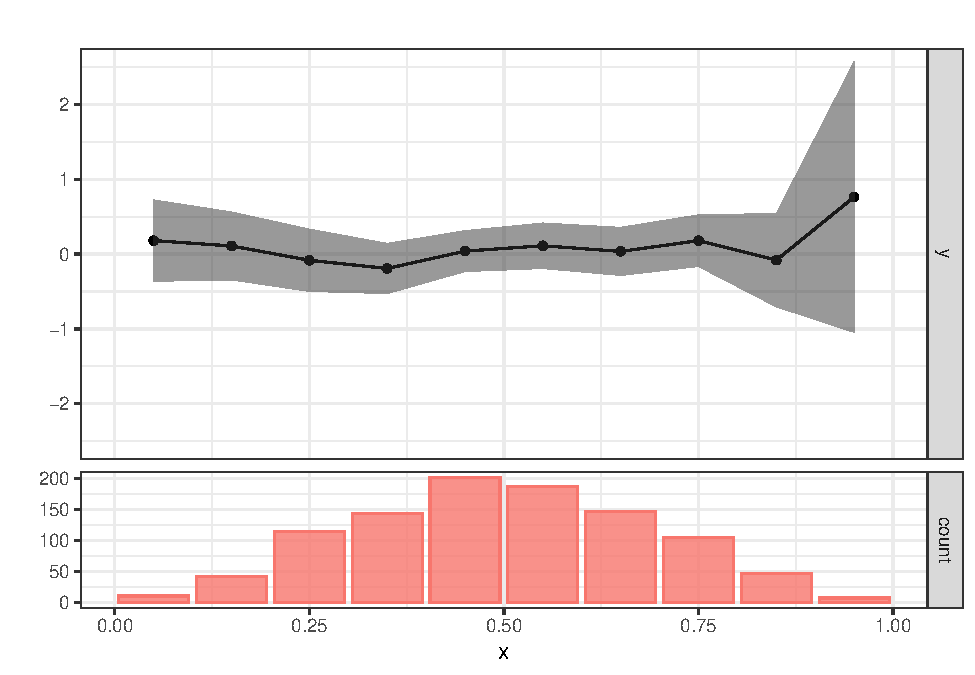
\includegraphics[width=0.5\linewidth]{_main_files/figure-latex/var-selection-3} }\subfloat[Positive effect - grouped\label{fig:var-selection-4}]{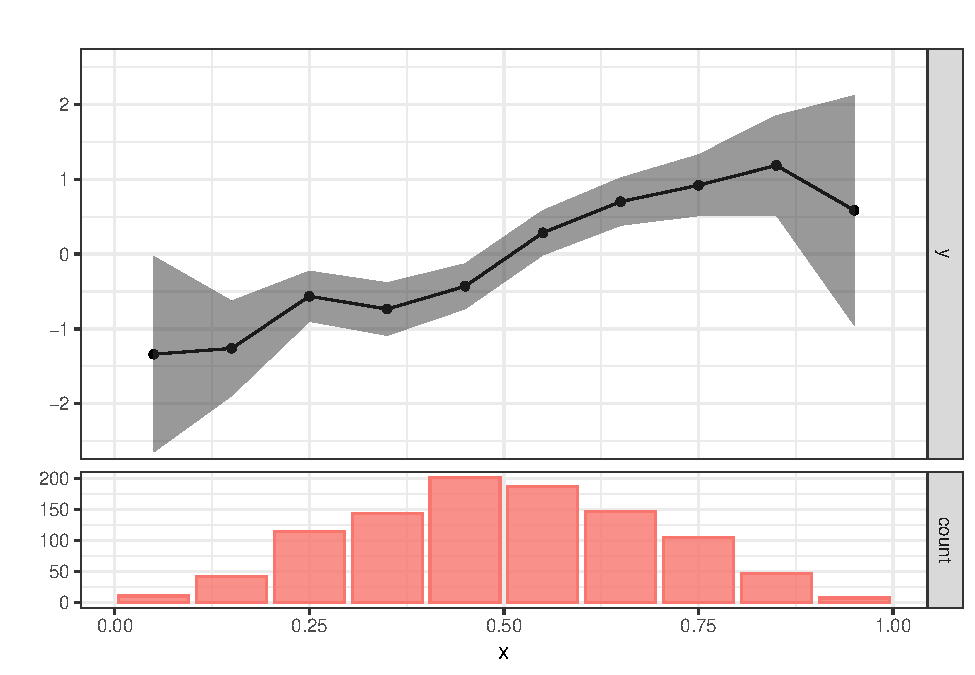
\includegraphics[width=0.5\linewidth]{_main_files/figure-latex/var-selection-4} }

}

\caption[Explanatory variable effect evaluation.]{Explanatory variable effect evaluation. The top-left and bottom-left panels represent a case in which \(x\) and \(y\) are not related, while the top-right and bottom-right panels represent a case of positive correlation. From the ungrouped plot in the top-right panel the effect is not clear, while from bottom-right panel it is evident.}\label{fig:var-selection}
\end{figure}

If we are dealing with a multivariate model where we already inserted the variables \(x_1, \dots, x_p\) and we want to evaluate the additional information brought by \(x_{p+1}\), it is possible to look at the plot \((x_{i, p+1}, r_i)\), where \(r_i\) are the residuals of the model without the variable \(x_{p+1}\):
\[
r_i = y_i - \hat{\mu}_i = y_i - g^{-1}\left( \hat{\beta}_0 + \hat{\beta}_1 x_{i1} + \dots + \hat{\beta}_p x_{ip} \right), \quad i\in\{1,2,\dots,n\}
\]

If the plot shows a clear trend, we will add the variable \(x\) to the model, otherwise we won't.

The choice of adding or not a variable in the model can be supported by \emph{hypothesis testing}. Given a GLM with coefficients \(\beta_0, \beta_1, \dots, \beta_p\), it is possible to test if a group of coefficients \(\beta_{j_1}, \beta_{j_2}, \dots, \beta_{j_s}\) is equal to zero. Formally the hypotheses tested are:
\[
\begin{cases}
H_0: & \beta_{j_k} = 0 \ \forall k \in \{1, 2, \dots, s\} \\
H_1: & \exists k: \beta_{j_k} \neq 0
\end{cases}
\]

If the hypothesis \(H_0\) is accepted, the variables \(x_{j_1}, x_{j_2}, \dots, x_{j_s}\) can be removed from the model; if the hypothesis \(H_0\) is rejected, at least some of the variables \(x_{j_1}, x_{j_2}, \dots, x_{j_s}\) should be kept in the model.

If we want to test if a quantitative variable \(x_j\) has a significant effect, we can conduct the test on the single coefficient \(\beta_j\). If we want to test if a qualitative variable with dummy encoding \(x_{j_1}, x_{j_2}, \dots, x_{j_s}\) is significant, we can conduct the test on the coefficients \(\beta_{j_1}, \beta_{j_2}, \dots, \beta_{j_s}\). For qualitative variables it is also possible to conduct a test for each level \(x_{j_k}\); in this case we would test one by one if each level has an effect that is significantly different form the base level effect.

To conduct the test it is possible to use several statistics. One of them is the test based on \emph{log likelihood ratio}. Let's indicate with \(\hat{\boldsymbol{\beta}}\) the estimated coefficients from the model without any constraint and with \(\hat{\boldsymbol{\beta}}^{(0)}\) the estimated coefficients with the constraints defined by \(H_0\). As the space \(\hat{\boldsymbol{\beta}}^{(0)}\) belongs to is a subset of the space \(\hat{\boldsymbol{\beta}}\) belongs to, it results:
\[
L\left(\hat{\boldsymbol{\beta}}^{(0)}\right) \le L\left(\hat{\boldsymbol{\beta}}\right)
\]
and then:
\[
\frac{L\left(\hat{\boldsymbol{\beta}}^{(0)}\right)}{L\left(\hat{\boldsymbol{\beta}}\right)} \le 1
\]

The basic idea is that, if the variables \(x_{j_1}, x_{j_2}, \dots, x_{j_s}\) have a significant effect, \(L\left(\hat{\boldsymbol{\beta}}\right)\) will be much higher than \(L\left(\hat{\boldsymbol{\beta}}^{(0)}\right)\) and we will reject the hypothesis \(H_0\), while if the variables \(x_{j_1}, x_{j_2}, \dots, x_{j_s}\) have not a significant effect, \(L\left(\hat{\boldsymbol{\beta}}\right)\) will be more or less the same as \(L\left(\hat{\boldsymbol{\beta}}^{(0)}\right)\) and we will accept the hypothesis \(H_0\).

To perform the test, the quantity usually employed is the following:
\begin{align*}
\lambda & = -2 \log{\left( \frac{L\left(\hat{\boldsymbol{\beta}}^{(0)}\right)}{L\left(\hat{\boldsymbol{\beta}}\right)} \right)} \\
& = -2 \left[ \ell\left(\hat{\boldsymbol{\beta}}^{(0)}\right) - \ell\left(\hat{\boldsymbol{\beta}}\right) \right]
\end{align*}

If we indicate \(\tilde{\lambda} = -2 \left[ \ell\left(\tilde{\boldsymbol{\beta}}^{(0)}\right) - \ell\left(\tilde{\boldsymbol{\beta}}\right) \right]\), it is possible to demonstrate that, under the hypothesis \(H_0\), \(\tilde{\lambda}\) has approximately chi-squared distribution with \(s\) degrees of freedom:
\[
\tilde{\lambda} \dot\sim \chi^2(s)
\]

Therefore, with a significance level \(\alpha\) we will reject \(H_0\) when \(\lambda > \chi_{s, 1-\alpha}\), where \(\chi_{s, 1-\alpha}\) is the quantile of order \(1-\alpha\) of the distribution \(\chi^2(s)\).

The same approach can be used in general for testing hypotheses that can be expressed as \(H_0: \boldsymbol{L}\boldsymbol{\beta} = \xi\), where \(\boldsymbol{L}\) is a matrix \(s\times(p+1)\) and \(\xi\in\mathbb{R}^{p+1}\). This is particularly useful in qualitative variables to test if some of the levels have the same effect and can be then unified. For example, if \(x_{j_1}\) and \(x_{j_2}\) are two dummy variables that describe two levels of the same quantitative variable, we can perform the test \(H_0: \beta_{j_1} = \beta_{j_2}\) in order to decide whether unifying the two levels is suitable or not.

Anyway, selecting the variables by performing hypotheses testing have some drawbacks. First of all, conducting a lot of test produce the multiple test problem. Let's consider the case in which we conduct a test of the kind \(H_0: \beta_j = 0\) with a significance level \(\alpha=0.05\) on many variables that have no effect on the response. On average, although the null hypotheses are always true, we will reject them once every 20 tests. That means that if we have available 100 variables, we will randomly select 5 of them, falling in \emph{overfitting}. To fix this problem, it is possible to use the Bonferroni correction, that consist in dividing \(\alpha\) by the number of test conducted to define the rejection region. But this could be a too restrictive correction that could lead to discard from the model some useful variables, falling in \emph{underfitting}.

Moreover, hypothesis testing aim is finding whether data supports or not an hypothesis. If the aim of the model is prediction, basing variable selection on hypotheses testing could lead to a sub-optimal model.

Another method for variable selection is comparing the models by computing \emph{information criteria}. Two information criteria commonly used are the \emph{Akaike Information Criterion} (AIC) and the \emph{Bayesian Information Criterion} (BIC):
\begin{align*}
AIC & = -2\ell(\boldsymbol{\beta}) + 2 (p+1) \\
BIC & = -2\ell(\boldsymbol{\beta}) + \log(n) (p+1)
\end{align*}

The aim of these statistics is to penalize the likelihood by adding a component that measures the complexity of the model. Among the models considered, the optimal model will be the one that minimizes the information criterion. Thus, if two models have the same likelihood, the optimal model will be the one with less parameters. If the model with more parameter has a higher likelihood, it will be chosen only if that increase in likelihood compensated the increase in complexity.

Another way to compute model predictive performance is by randomly splitting the available dataset \(\mathcal{D} = \left\{ (\boldsymbol{x}_1, \omega_1, y_1), \dots, (\boldsymbol{x}_n, \omega_n, y_n) \right\}\) into a \emph{training set} (or learning set) \(\mathcal{D}^{\mathcal{B}}\) and a \emph{test set} \(\mathcal{D}^{\bar{\mathcal{B}}}\), with \(\mathcal{B}\subset\{1,2,\dots,n\}\) labeling the dataset \(\mathcal{D}^{\mathcal{B}} = \left\{ (\boldsymbol{x}_i, \omega_i, y_i): i \in \mathcal{B} \right\} \subset \mathcal{D}\) and \(\bar{\mathcal{B}} = \{1, 2, \dots, n\} \setminus \mathcal{B}\). With this split, we can fit the model on only the training set \(\mathcal{D}^{\mathcal{B}}\) and assess its performance on the test set \(\mathcal{D}^{\bar{\mathcal{B}}}\) by computing the deviance \(D\left( \hat{\boldsymbol{\beta}}^{\mathcal{B}}, \boldsymbol{y}^{\bar{\mathcal{B}}} \right)\), where \(\hat{\boldsymbol{\beta}}^{\mathcal{B}}\) is the vector of the coefficients estimated on the training set and \(\boldsymbol{y}^{\bar{\mathcal{B}}}\) is the vector of the observed response variables in the test set. This way it is possible to choose the best model as the one that minimize the deviance in the test set and then fitting it with the whole dataset \(\mathcal{D}\).

A limit of the train-test approach is that it could bring to overfitting in the test set. Indeed, in particular if the dataset is small, it is possible that a specific set of variables minimizes the deviance on the test set just by chance. To prevent this, it is possible to conduct a \emph{K-fold cross validation}. This consists in randomly partitioning the dataset \(\mathcal{D}\) into \(K\) subsets \(\mathcal{D}^{\mathcal{B}_1}, \mathcal{D}^{\mathcal{B}_2}, \dots, \mathcal{D}^{\mathcal{B}_K}\) and, for each subset \(\mathcal{D}^{\mathcal{B}_k}\), performing a train-test procedure keeping \(\mathcal{D}^{\setminus \mathcal{B}_k} = \mathcal{D} \setminus \mathcal{D}^{\mathcal{B}_k}\) as a training set and \(\mathcal{D}^{\mathcal{B}_k}\) as a test set. For each \(k\) we can compute the testing deviance \(D\left( \hat{\boldsymbol{\beta}}^{\setminus \mathcal{B}_k}, \boldsymbol{y}^{\mathcal{B}_k} \right)\). We can then compute the average deviance within the \(K\) subset as:
\[
D^{CV(K)} = \frac{1}{K} \sum_{k=1}^{K}{D\left( \hat{\boldsymbol{\beta}}^{\setminus \mathcal{B}_k}, \boldsymbol{y}^{\mathcal{B}_k} \right)}
\]
Thus, the best model will be the one that minimize \(D^{CV(K)}\).

The higher \(K\) is, the less subjected to randomness \(D^{CV(K)}\) is. However, the higher \(K\) is, the more computationally expensive the procedure is. A common choice for \(K\) is \(K=10\). If we choose \(K=n\), the procedure is also called \emph{leave-one-out cross validation}.

\hypertarget{scalability-and-manual-fitting}{%
\subsubsection{Scalability and manual fitting}\label{scalability-and-manual-fitting}}

One problem of GLM is that the variables selection process is not so easily scalable. Indeed, if we consider \(p\) explanatory variables, even without taking into account interactions and quantitative variables transformation, there are \(2^p\) possible models that can be obtained by choosing a subset of those variables. As \(p\) increases, building all these models and choosing the optimal one becomes unfeasible.

One strategy to reduce the time consumption is to use a \emph{stepwise procedure}. First of all we must choose a criterion to compare the models, such as the AIC. Then we have to choose a starting model that consider the variables subset \(\mathcal{C}_0 \subset \{ 1,2,\dots,p \}\). It is possible to compare this model with all the models that can be obtained by removing one variable from \(\mathcal{C}_0\) or adding to \(\mathcal{C}_0\) one that is not included in it. From all these models we can compute the AIC and we will choose as \(\mathcal{C}_1\) the set of variables that minimize the AIC. If none of the considered model has an AIC lower to the one obtained with the variables \(\mathcal{C}_0\), the procedure ends and our final set of variables is \(\mathcal{C}_0\). Otherwise, we will repeat the step with \(\mathcal{C}_1\). The procedure can be iteratively repeated until we obtain a subset of variables \(\mathcal{C}_f\) that can't be improved by removing or adding a variable. The model with the variables \(\mathcal{C}_f\) will be our chosen one.

This procedure is much faster than computing all the \(2^p\) models, but it is still not so scalable for large \(p\). Moreover, in this procedure we are not taking into account the interactions and the possible transformations for the quantitative variables. This can be achieved by slightly modifying the algorithm, but it would further increase the complexity and the time consumption. Another option is starting from the result of the stepwise regression and manually choosing interactions and quantitative variables transformations by looking at plots as described in \ref{chap:var-effects}.

One characteristic of GLM is that the variables effects can be easily interpreted and the variable selection process is for large part manual. This aspect can be problematic if there are a lot of explanatory variables, but it brings some important benefits too. Indeed, the actuary can take choices on variable selection not only based on observed data, but also on his domain knowledge. For instance, the choice of selecting or not an explanatory variable can be guided also on its interpretation: if the observed effect makes sense, it can be added to the model even if it is not statistically significant and it doesn't decrease the AIC, and, on the opposite, if the observed effect is not reasonable, the actuary can choose not to insert the variable in the model even if its effect is supported by the data. So, in the actuarial practice, in the GLM fitting process there is always a subjective component that impacts on the final result. For these reason it is important for the actuary to have a deep knowledge on the phenomenon he is modeling.

An aspect that facilitates the model building and reduces the complexity of the process, even if there are many variables, is that usually the models are not built from scratch. Actuarial models are usually updated once a year, so it is also possible to start the new model by fitting on new data the final model from the year before. As the models are usually built with policies data from more than one year, the new dataset partially overlaps with the one from the previous year. However, the overlapping observations aren't identical: the new dataset will have the new settlement information and some new explanatory variables. Anyway, if the actuary is familiar with the effects of the variables in the previous models, he already knows which will probably be relevant and which don't even deserve too much attention.

\newpage

\hypertarget{chap:gam}{%
\subsection{GAM}\label{chap:gam}}

In section \ref{chap:var-effects} we have seen that sometimes quantitative variables have not a linear effect on the linear predictor. In GLM it is possible to deal with non-linear effects by adding polynomial or split-wise terms. GAMs are models based on GLM that introduce a more flexible way to deal with quantitative variables with non-linear effects.

\hypertarget{model-assumptions}{%
\subsubsection{Model assumptions}\label{model-assumptions}}

In GAM, the assumptions are the same of GLM, stated in \ref{chap:glm-assumptions}, with the following advancement in the linear predictor:
\[
g(\mu_i) = \eta_i = \boldsymbol{x}_i^t \boldsymbol{\beta} + \sum_{l=1}^{q}{f_l(z_{i,l})}, \qquad i\in\{1,2,\dots,n\}
\]
where

\begin{itemize}
\tightlist
\item
  \(\boldsymbol{x}_i\) is the vector of the variables with a linear effect as described in GLM, that also include a term \(1\) that represents the intercept;
\item
  \(\boldsymbol{\beta}\) is the vector of the linear coefficients as described in GLM;
\item
  \(z_{i,1}, z_{i,2}, \dots, z_{i,q}\) are the quantitative variables with a non linear effect;
\item
  \(f_1(\cdot), f_2(\cdot), \dots, f_q(\cdot)\) are continuous functions with continuous first and second derivatives.
\end{itemize}

The functions \(f_l(\cdot)\) introduce the possibility to model non-linear effects of the variables \(z_l\).

\hypertarget{chap:cubic-splines}{%
\subsubsection{Cubic splines}\label{chap:cubic-splines}}

A class of functions commonly used for modeling \(f_l(\cdot)\) is the class of the \emph{cubic splines}.

\begin{definition}[Cubic Splines]
\label{def:cubic-splines} \iffalse (Cubic Splines) \fi{} Let consider \(m\) real numbers \(\nu_1, \nu_2, \dots, \nu_m\), called \textit{knots}, and a function \(f:[\nu_1, \nu_m] \to \mathbb{R}\) such that:
\[
f(x) = h_t(x), \qquad x\in[\nu_t, \nu_{t+1}[
\]
where, for \(t = 1, 2, \dots, m-1\), \(h_t(x) = \alpha_t + \vartheta_t x + \gamma_t x^2 + \delta_t x^3\). For the last index \(m-1\), \(f(x) = h_{m-1}(x)\) is extended to \([\nu_{m-1}, \nu_{m}]\).

\(f(x)\) is a \textit{cubic spline} if it satisfies the following conditions in the internal knots \(\nu_2, \nu_3, \dots, \nu_{m-1}\)
\begin{equation}
\label{eq:cubic-spline-constraints}
h_{t-1}(\nu_t) = h_{t}(\nu_t), \qquad h'_{t-1}(\nu_t) = h'_{t}(\nu_t), \qquad h''_{t-1}(\nu_t) = h''_{t}(\nu_t)
\end{equation}
\end{definition}

The constraints for \(f(\cdot)\) make it a continuous functions with first and second derivatives continuous in \(]\nu_1, \nu_m[\). It is possible to extend the cubic spline \(f(\cdot)\) to an interval \([a, b] \supset [\nu_1, \nu_m]\) with linear extensions on \([a, \nu_1[\) and \(]\nu_m, b]\). The so built function \(f:[a,b]\to\mathbb{R}\) is called \emph{natural cubic spline}.

In definition \ref{def:cubic-splines} we introduced 4 parameters (\(\alpha_t, \vartheta_t, \gamma_t, \delta_t\)) for each of the \(m-1\) intervals \([\nu_t, \nu_{t+1}[\), \(t\in\{1,2,\dots,m-1\}\). So, we have \(4(m-1)\) parameters. In equation \eqref{eq:cubic-spline-constraints} we introduced \(3\) constraints for each of the \(m-2\) knot in \(\nu_2, \nu_3, \dots, \nu_{m-1}\). So the free parameters become \(4(m-1) - 3(m-2) = m+2\). The linear extension on \([a, \nu_1[\) and \(]\nu_m, b]\) corresponds to the constraint \(f''(x)=0\) on \([a, \nu_1[ \, \cup \, ]\nu_m, b]\), thus, \(h''_1(\nu_1)=0\) and \(h''_m(\nu_m)=0\). Adding these two constraints, we get that the natural cubic spline \(f:[a,b]\to\mathbb{R}\) has \(m\) degrees of freedom.

With an approach similar to the one we used in \ref{chap:var-effects} for split-wise effects in GLM, we can represent a cubic spline by the functions \(x \mapsto \left( x-\nu_t \right)_+^3\), \(t=1,2,\dots,m\).

The expression:
\begin{equation}
\label{eq:cubic-spline-decomposition}
f(x) = \alpha_0 + \vartheta_0 x + \sum_{t=1}^{m}{c_t \left( x-\nu_t \right)_+^3}, \qquad \text{with} \quad \sum_{t=1}^{m}{c_t} = 0 \quad \text{and} \quad \sum_{t=1}^{m}{c_t\nu_t} = 0
\end{equation}
gives a natural cubic spline.

The two side constraints ensure that we have a smooth linear extension above \(\nu_m\). The expression \eqref{eq:cubic-spline-decomposition} presents \(m+2\) parameters, thus, with the 2 side constraints, there are \(m\) degrees of freedom. From this expression it is easy to show that the natural cubic splines over the interval \([a,b]\) with knots \(\nu_1, \nu_2, \dots, \nu_m\) constitute a \(m\)-dimensional vectorial space.

\hypertarget{smoothing}{%
\subsubsection{Smoothing}\label{smoothing}}

If we try to fit a cubic spline on data, we find that by increasing the number of knots, the function tends to overfit data. This is due to the fact that, increasing the number of knots, we are increasing the number of parameters of the model and, thus, the variance of the parameters estimators increases. We can see this effect in figure \ref{fig:cub-spline}.







\begin{figure}[!hbtp]

{\centering \subfloat[$0$ knots\label{fig:cub-spline-1}]{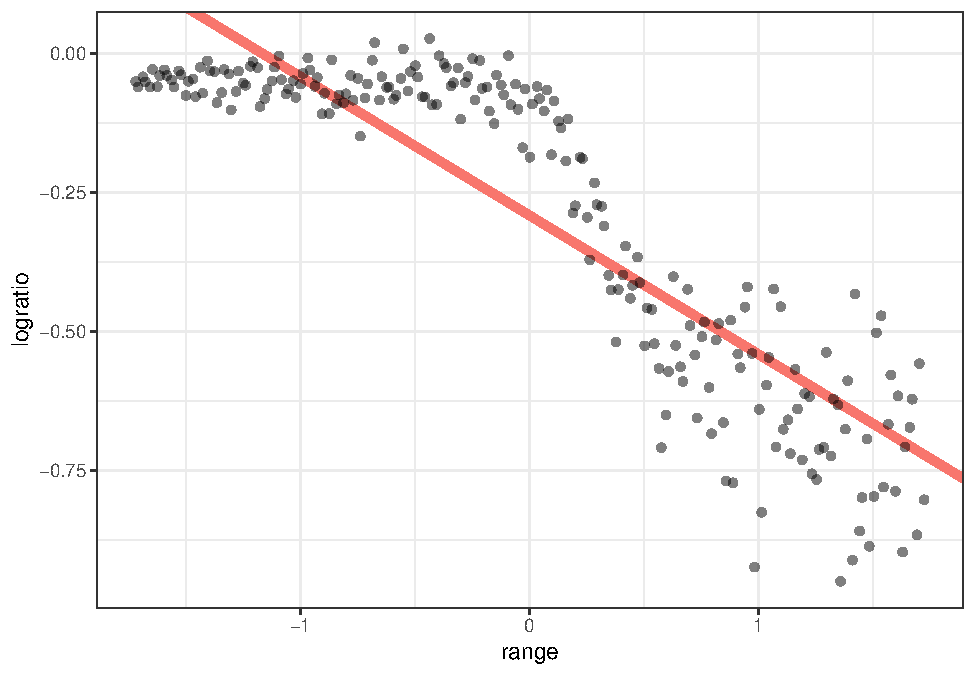
\includegraphics[width=0.5\linewidth]{_main_files/figure-latex/cub-spline-1} }\subfloat[$3$ knots\label{fig:cub-spline-2}]{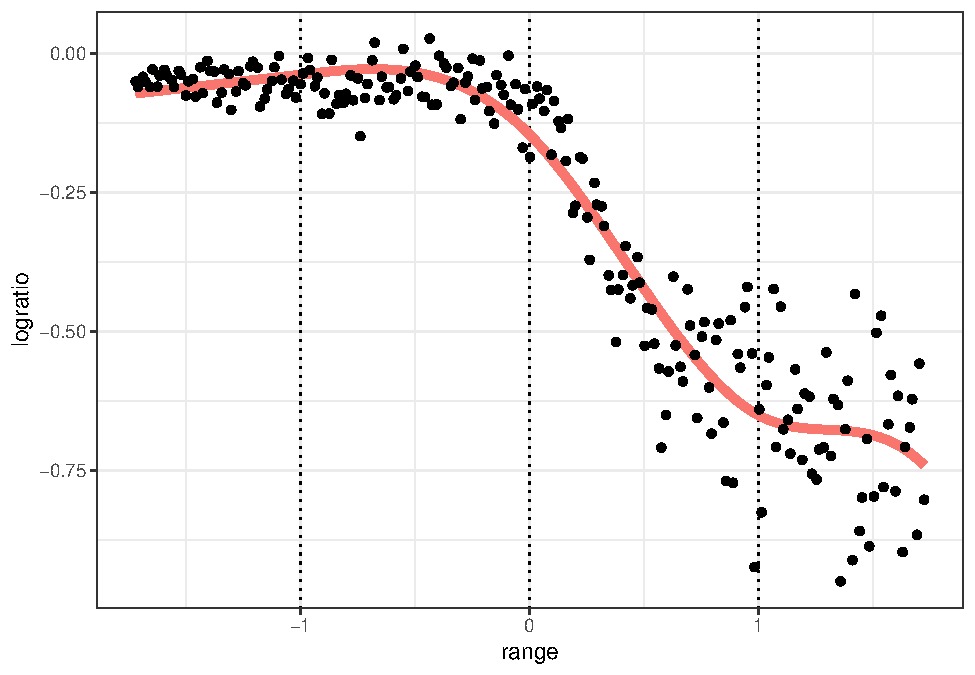
\includegraphics[width=0.5\linewidth]{_main_files/figure-latex/cub-spline-2} }\newline\subfloat[$7$ knots\label{fig:cub-spline-3}]{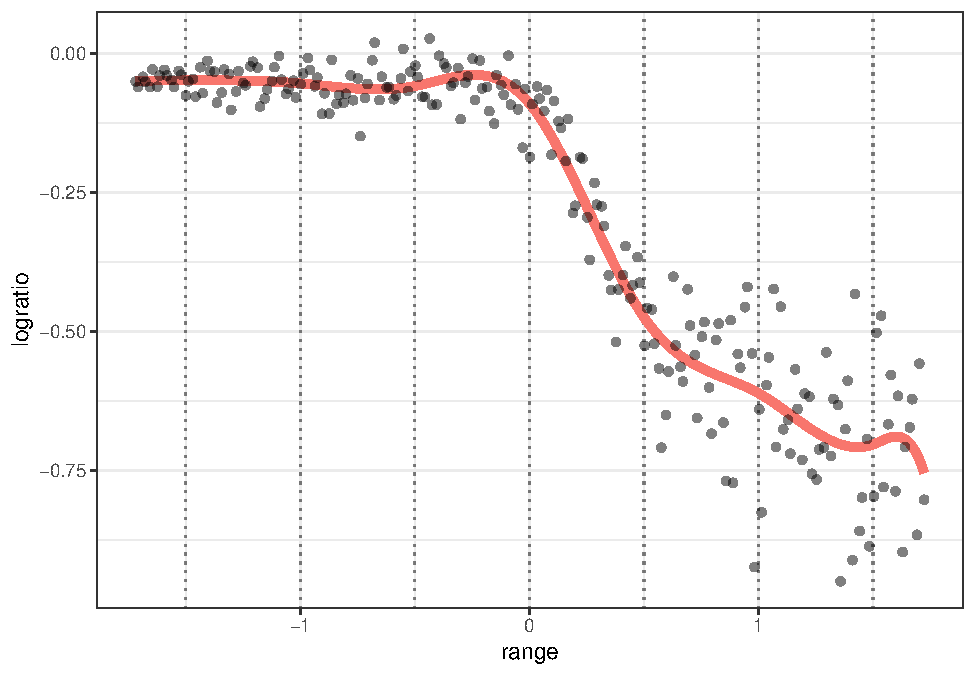
\includegraphics[width=0.5\linewidth]{_main_files/figure-latex/cub-spline-3} }\subfloat[$35$ knots\label{fig:cub-spline-4}]{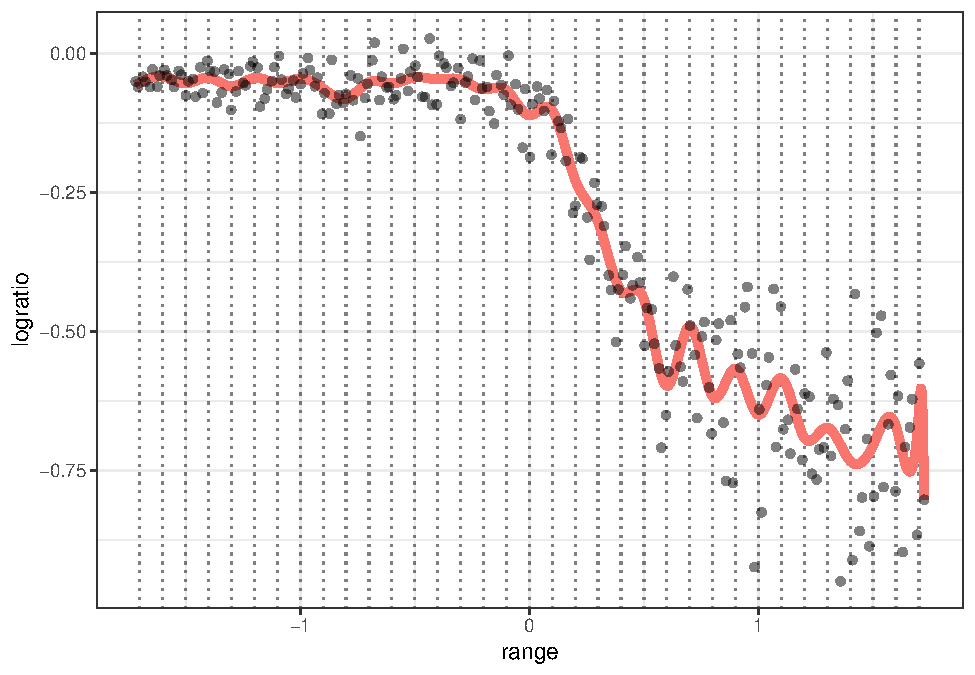
\includegraphics[width=0.5\linewidth]{_main_files/figure-latex/cub-spline-4} }

}

\caption[GLM with cubic splines for different numbers of knots.]{GLM with cubic splines for different numbers of knots. The more knots there are, the wigglier the estimated function \(\hat{f}(x)\) is.}\label{fig:cub-spline}
\end{figure}

In the top-left panel, the model fitted is just linear and it clearly doesn't follow the path made by the observed points. In the bottom-right panel, the models fitted is a spline with 35 knots and it is clearly too wiggly compared to the path made by the observed points.

A measure of the wiggliness of a function is given by the integral of its squared second derivative:
\begin{equation}
\label{eq:wiggliness}
\int_{a}^{b}{\left( f''(x) \right)^2 dx}
\end{equation}

In figure \ref{fig:wiggliness} some examples of functions \(f(x)\) and their squared second derivatives \(\left(f''(x)\right)^2\) are represented. In the top panels, four functions of increasing wiggliness are represented and, in the bottom panels, we can see their four squared second derivatives.





\begin{figure}[!hbtp]

{\centering 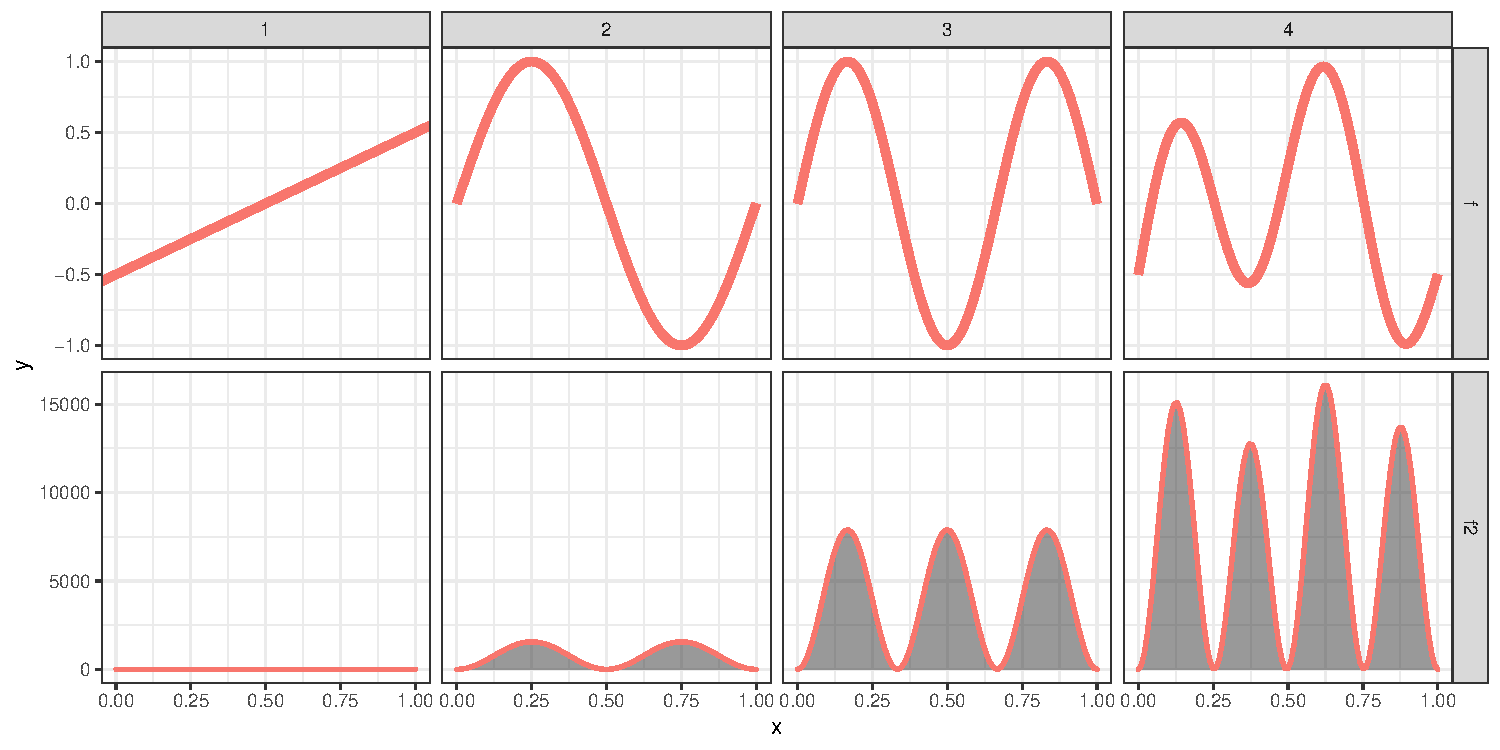
\includegraphics[width=1\linewidth]{_main_files/figure-latex/wiggliness-1} 

}

\caption[\(\left(f''(x)\right)^2\) for functions with different wiggliness.]{\(\left(f''(x)\right)^2\) for functions with different wiggliness. The wigglier the function \(f(x)\) is, the higher \(\left(f''(x)\right)^2\) is.}\label{fig:wiggliness}
\end{figure}

As we can see from the plots, if a function \(f(x)\) is linear, \(\left(f''(x)\right)^2\) is null and, as the curvature of the function increases, \(\left(f''(x)\right)^2\) increases. For this reason, \(\left(f''(x)\right)^2\) can also be seen as a measure of how much \(f(x)\) differs from a linear function.

What is done in GAM to contain this wiggliness and to prevent overfitting is taking into account a penalization based on \(\left(f''(x)\right)^2\). If we have a regression problem with one explanatory variable \(x\), this can be achieved by considering the minimization problem in \eqref{eq:max-lik-est-deviance} and adding a penalization term to the deviance:
\begin{equation}
\label{eq:gam-est-deviance}
\hat{f} = \argmin_{f}{\left\{D(f, \boldsymbol{y}) + \lambda \int_{a}^{b}{\left( f''(x) \right)^2 dx}\right\}}
\end{equation}

In the notation of the formula \eqref{eq:gam-est-deviance} we used \(f\) to indicate all the parameters of the natural cubic spline. The hyper-parameter \(\lambda\ge0\) is called \emph{smoothing parameter}. It measures how much we want to penalize wiggliness. If we choose \(\lambda=0\) we won't penalize for \(\left( f''(x) \right)^2\) and the optimization problem corresponds to the maximum likelihood. The higher \(\lambda\) is, the more penalization for \(\left( f''(x) \right)^2\) we introduce and the smoother the estimate \(\hat{f}(x)\) will be. If \(\lambda\to+\infty\), we will introduce an infinite penalization for wiggliness, so the result will have \(\hat{f}''(x)=0\), thus \(\hat{f}(x)\) will be linear. An example with different levels of \(\lambda\) can be seen in figure \ref{fig:gam-lambda}.







\begin{figure}[!hbtp]

{\centering \subfloat[$\lambda = 0$\label{fig:gam-lambda-1}]{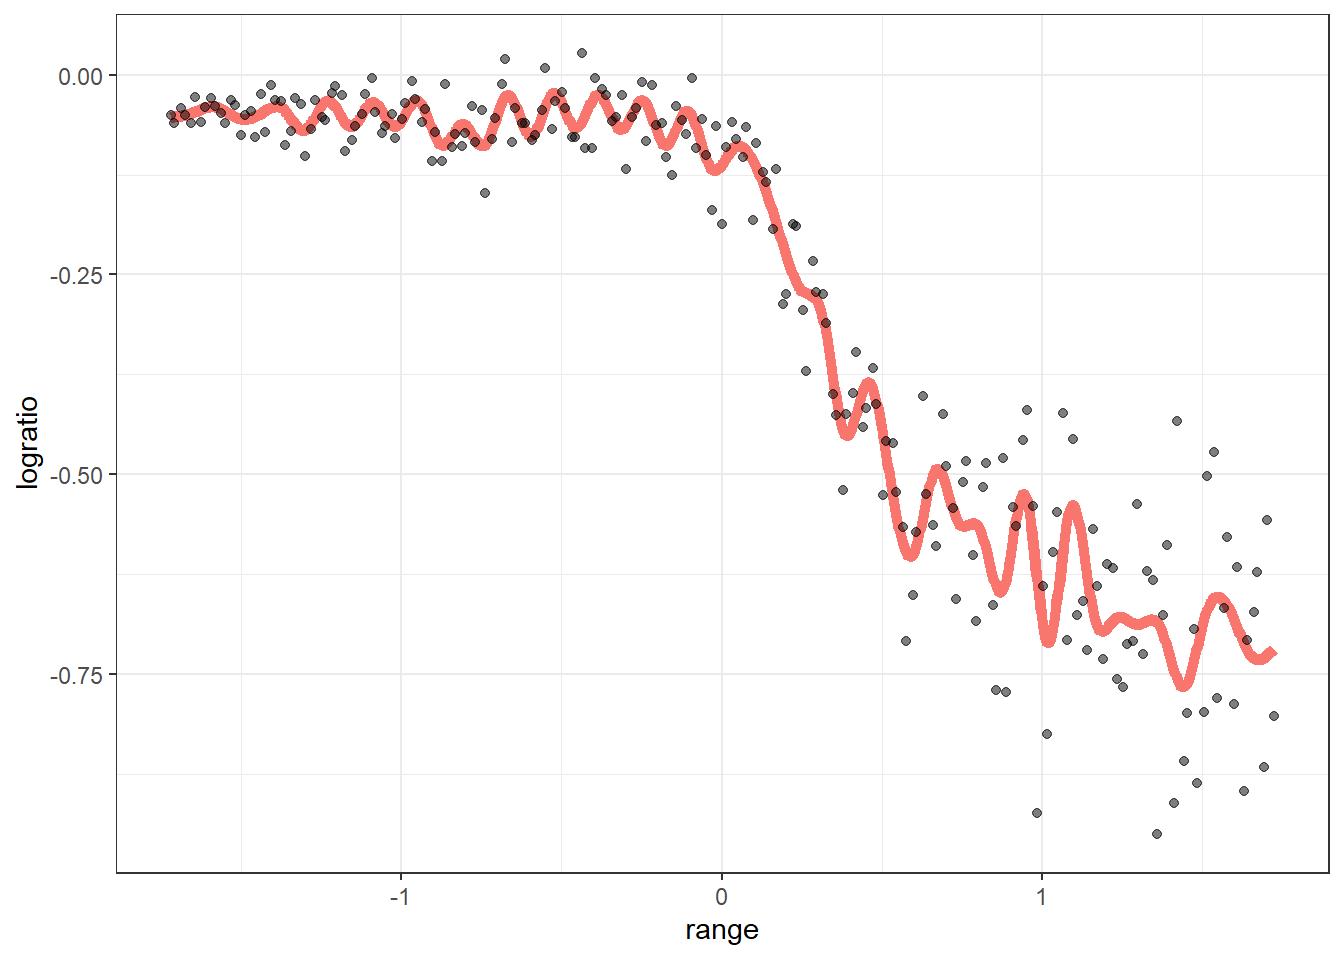
\includegraphics[width=0.5\linewidth]{_main_files/figure-latex/gam-lambda-1} }\subfloat[$\lambda = 10$\label{fig:gam-lambda-2}]{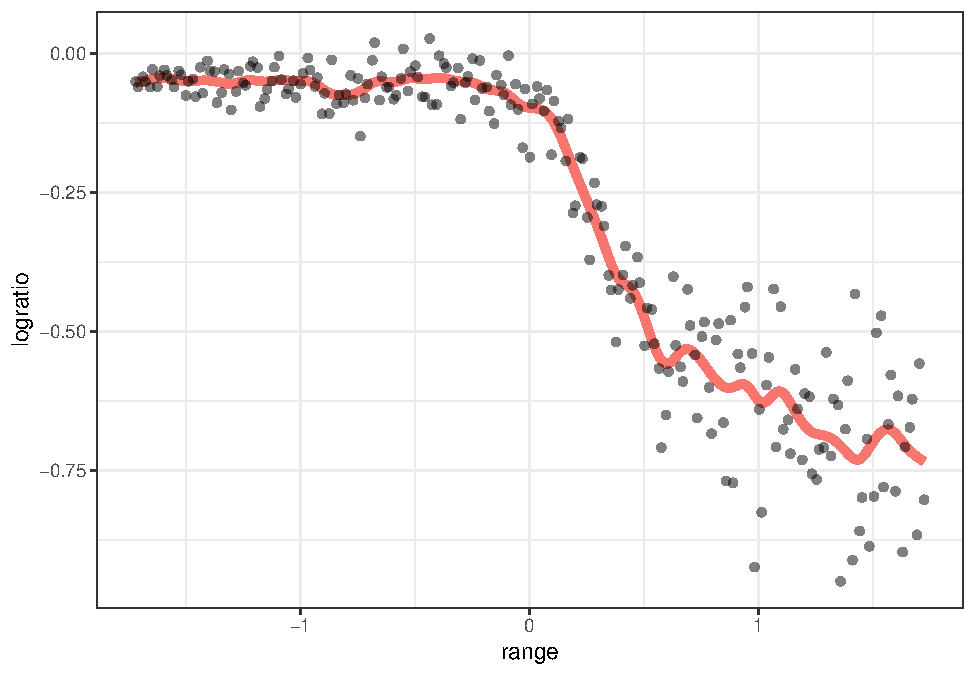
\includegraphics[width=0.5\linewidth]{_main_files/figure-latex/gam-lambda-2} }\newline\subfloat[$\lambda = 10^3$\label{fig:gam-lambda-3}]{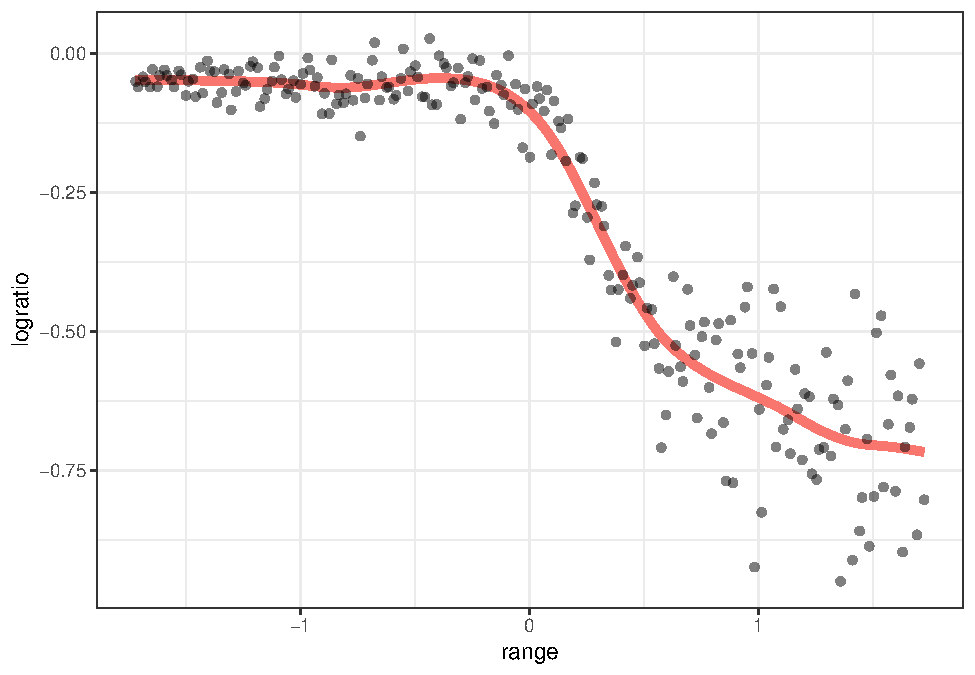
\includegraphics[width=0.5\linewidth]{_main_files/figure-latex/gam-lambda-3} }\subfloat[$\lambda = 10^6$\label{fig:gam-lambda-4}]{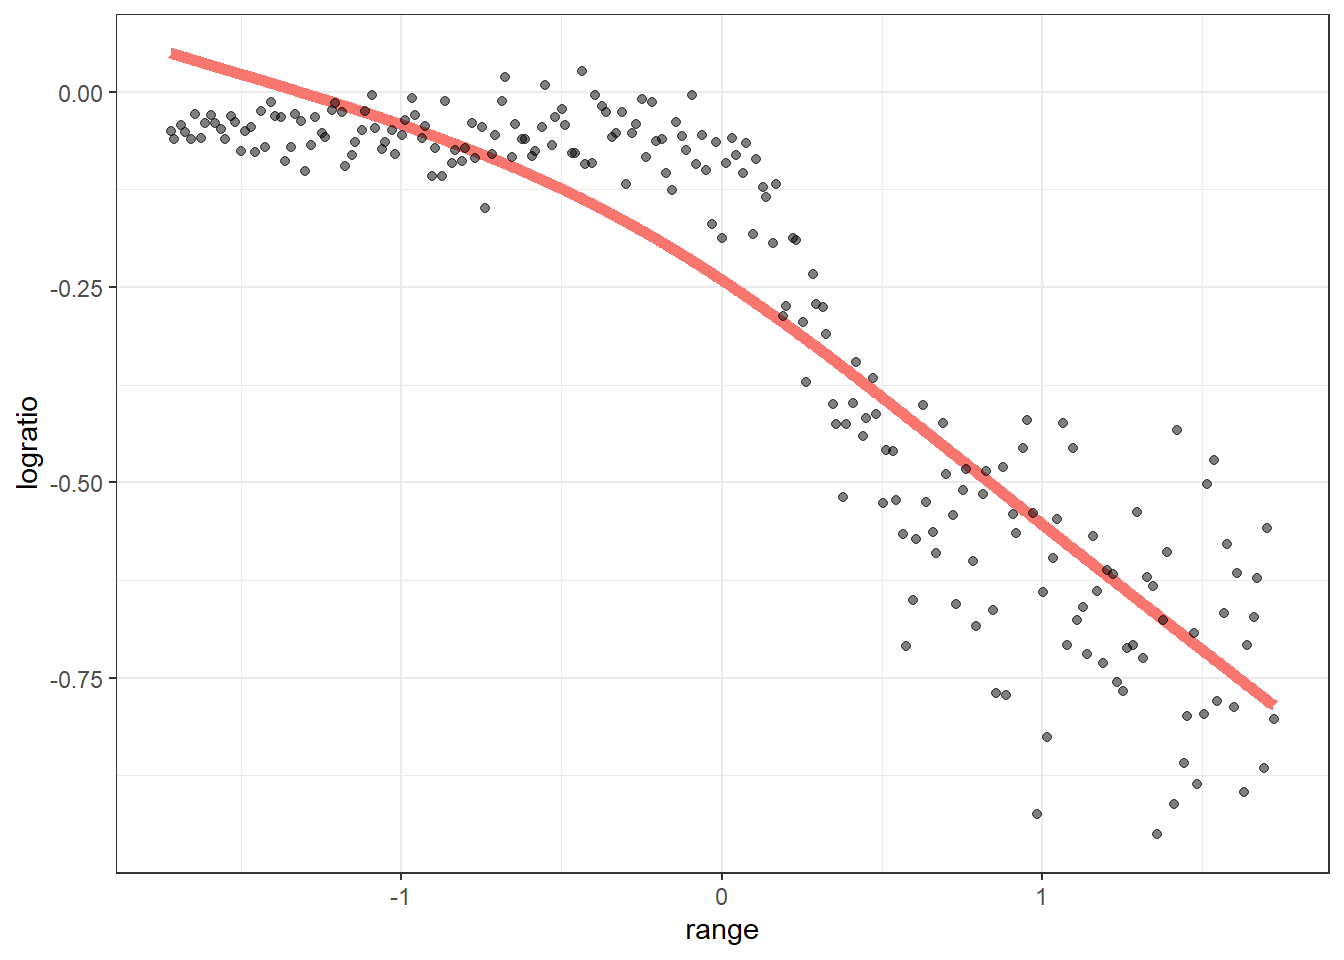
\includegraphics[width=0.5\linewidth]{_main_files/figure-latex/gam-lambda-4} }

}

\caption[GAM estimate \(\hat{f}(x)\) for different levels of the smoothing parameter \(\lambda\).]{GAM estimate \(\hat{f}(x)\) for different levels of the smoothing parameter \(\lambda\). The higher \(\lambda\) is, the less wiggly the estimated function \(\hat{f}(x)\) is.}\label{fig:gam-lambda}
\end{figure}

All the models has been fitted with \(m = 50\) knots. As we can see, with \(\lambda = 0\) we are clearly overfitting observations, while with \(\lambda = 10^6\) we are clearly underfitting them.

As soon as the number of knots \(m\) is large enough, the exact number \(m\) and the positioning of the knots \(\nu_1, \nu_2, \dots, \nu_m\) is not important. If the function is flexible enough, the tuning of the curve is done by just tuning \(\lambda\). It is possible to use as many knots as the determinations of \(x\) are, but it could be too computationally expensive. A possible choice is to fix a number of knots \(m\) and positioning \(\nu_1, \nu_2, \dots, \nu_m\) on empirical quantiles of the observed \(x\) or equally spaced in the range of \(x\). In our example, \(m=50\) knots seems to be large enough.

In general, if we have \(q\) quantitative explanatory variables that we want to fit with splines, the formula \eqref{eq:gam-est-deviance} becomes:
\begin{equation}
\label{eq:gam-est-deviance-multi}
\boldsymbol{\hat{f}} = \argmin_{\boldsymbol{f}}
{\left\{
  D(\boldsymbol{f}, \boldsymbol{y})
    + \sum_{l=1}^{q}{
      \lambda_l \int_{a_l}^{b_l}{\left( f_l''(x_l) \right)^2 dx}
    }
\right\}
} 
\end{equation}
where \(\boldsymbol{f} = \left( f_1, f_2,\dots,f_q \right)\).

In this context, we have to tune a vector of \(q\) smoothing parameters:
\[\boldsymbol{\lambda} = \left( \lambda_1, \lambda_2, \dots, \lambda_q \right)\]

\hypertarget{chap:gam-choice-lambda}{%
\subsubsection{Choice of the smoothing parameters}\label{chap:gam-choice-lambda}}

As described, the selection of the \(x_l\) effect consists just in finding the optimal parameter \(\lambda_l\). The technique commonly used in machine learning for hyper-parameter tuning is the \emph{Cross Validation}.

For a set \(\Lambda\) of values of \(\boldsymbol{\lambda}\) we can perform a K-fold cross validation as described in \ref{chap:variable-selection} and, for each \(\boldsymbol{\lambda}\in\Lambda\), we can compute the average test deviance:
\[
D^{CV(K)}_{\boldsymbol{\lambda}} =
\frac{1}{K} \sum_{k=1}^{K}{
D\left(
\boldsymbol{\hat{f}}_{\boldsymbol{\lambda}}^{\setminus \mathcal{B}_k}, \boldsymbol{y}^{\mathcal{B}_k}
\right)
}
\]
At this point, we will choose the hyper-parameter vector that minimizes the cross-validation deviance:
\[
\hat{\boldsymbol{\lambda}} = \argmin_{\boldsymbol{\lambda}\in\Lambda}{D^{CV(K)}_{\boldsymbol{\lambda}}}
\]

In particular if \(q\) is big, this procedure can be too computationally expensive. Two alternatives are the \emph{Generalized Cross Validation} (GCV) and the \emph{Un-Biased Risk Estimator} (UBRE). The idea behind these approaches is to estimate the test set deviance by just computing the training set deviance and applying to it a correction that penalizes for the complexity of the model, as it is done in AIC and BIC, described in section \ref{chap:variable-selection}.

GCV and UBRE formulas are based on the fact that GAMs with identity link and Normal response are \emph{linear smoothers}, i.e.~\(\boldsymbol{\hat{\mu}}\) can be expressed as:
\begin{equation}
\label{eq:linear-smoother}
\boldsymbol{\hat{\mu}} = H \boldsymbol{y}
\end{equation}
where \(H\) is a \(n\times n\) matrix that depends on the design matrix \(\boldsymbol{X}\) and the hyper-parameters. \(H\) is called \emph{smoothing matrix}. In general, if the link is not identity and the response is not Normal, GAM is not a linear smoother, but the formula \eqref{eq:linear-smoother} still holds up with a local approximation.

It can be proven that the trace of \(H\) measures the flexibility of the function. Indeed, in Linear Model \(H = \boldsymbol{X} \left( \boldsymbol{X}^t\boldsymbol{X} \right)^{-1}\boldsymbol{X}^t\) and \(\text{tr}(H) = \text{tr}\left( \boldsymbol{X} \left( \boldsymbol{X}^t\boldsymbol{X} \right)^{-1}\boldsymbol{X}^t \right) = p + 1\), that is the number of \emph{degrees of freedom} of the model. For this reason \(\text{tr}(H)\) is also called number of \emph{effective degrees of freedom} of the model. In GAM, as the smoothing parameter \(\lambda\) increases, the flexibility of the model decreases and \(\text{tr}(H)\) decreases.

For linear smoothers it can be proved that the \emph{leave one out cross validation} is:
\[
D^{CV(n)} = \frac{1}{n} \sum_{i=1}^{n}{\left( \frac{y_i - \hat{\mu}_i}{1 - H_{ii}} \right)^2}
\]
where \(H_{ii}\) is the \(i\)\textsuperscript{th} element of the diagonal of the smoothing matrix \(H\).

This formula is particularly convenient because it requires just the fit with the whole dataset and not one fit for each fold. Indeed, in the formula the quantities that must be computed are \(\mu_i\) and \(H_{ii}\), that both depend on the model fitted with the whole dataset.

This formula can be further simplified by replacing the values \(H_{ii}\) with their average \(\frac{\text{tr}(H)}{n}\). This way we get the GCV.
\begin{equation}
\label{eq:gcv}
GCV = \frac{1}{n} \sum_{i=1}^{n}{\left( \frac{y_i - \hat{\mu}_i}{1 - \frac{\text{tr}(H)}{n}} \right)^2}
\end{equation}

As for K-fold cross validation we can compute the GCV for different values of \(\boldsymbol{\lambda} \in \Lambda\) and choose the value \(\boldsymbol{\hat{\lambda}}\) that minimizes the GCV.

The formula \eqref{eq:gcv} can be expressed as:
\begin{align}
\nonumber
GCV & = \frac{1}{n} \sum_{i=1}^{n}{\left( \frac{y_i - \hat{\mu}_i}{1 - \frac{\text{tr}(H)}{n}} \right)^2} \\
\nonumber
& = \left( \frac{n}{n - \text{tr}(H)} \right)^2 \underbrace{\frac{\sum_{i=1}^{n}{\left( y_i - \hat{\mu}_i \right)^2}}{n}}_{=D(\boldsymbol{\hat{f}},\boldsymbol{y})} \\
\label{eq:gcv-gam}
& = \left( \frac{n}{n - \text{tr}(H)} \right)^2 D(\boldsymbol{\hat{f}},\boldsymbol{y})
\end{align}

The expression \eqref{eq:gcv-gam} generalizes the GCV to all the GAMs, also in the case in which the link is not identity and the response is not Normal.

To select the best value of \(\boldsymbol{\lambda}\), we can perform a similar procedure using the UBRE in place of the GCV. The UBRE is defined as:
\[
UBRE = \frac{1}{n} D(\boldsymbol{\hat{f}}, \boldsymbol{y}) - \phi + \frac{2}{n} \text{tr}(H)\phi 
\]

Using the UBRE instead the GCV is preferred when \(\phi\) is known, such as in Poisson regression case, in which \(\phi=1\).

\hypertarget{why-cubic-splines}{%
\subsubsection{Why cubic splines}\label{why-cubic-splines}}

In section \ref{chap:cubic-splines} we said that \emph{cubic splines} are commonly used for modeling \(f(\cdot)\) in GAMs. This choice comes from the following theorem.

\begin{theorem}[Spline property]
\label{thm:th-splines-property} \iffalse (Spline property) \fi{} Given the knots \(\nu_1, \nu_2, \dots, \nu_m\) and the values \(y_1, y_1, \dots, y_m\), for any \(a\le\nu_1\) and \(b\ge\nu_m\), only one natural cubic spline \(s(\cdot)\), such that \(s(\nu_k)=y_k, \ k\in \{1, \dots, m\}\), exists.

Moreover, given \(f(\cdot)\) a function two times differentiable with continuity, such that \(f(\nu_k)=y_k, \ k\in \{1, \dots, m\}\), then, for any \(a\le\nu_1\) and \(b\ge\nu_m\), it results
\[
\int_a^b{\left( s''(x)\right)^2 dx} \le \int_a^b{\left( f''(x)\right)^2 dx}
\]
\end{theorem}
One consequence of this theorem is that, within all the continuous function \(f(\cdot)\) with continuous first and second derivatives, the one that minimize the optimization problem \eqref{eq:gam-est-deviance} is always a natural cubic splines.

Let's consider the determinations \(x_1^* < x_2^* < \dots < x_m^*\) of the variable \(x\). If \(f(\cdot)\) is a continuous function with continuous first and second derivatives, for the theorem \ref{thm:th-splines-property}, there exists only one natural cubic spline \(s(\cdot)\) such that \(s(x_k^*) = f(x_k^*), \ k\in \{1, \dots, m\}\). As, \(s(x_i)=f(x_i) \ \forall i \in \mathcal{D}\), it results that \(D(s, \boldsymbol{y}) = D(f, \boldsymbol{y})\). As \(D(s, \boldsymbol{y}) = D(f, \boldsymbol{y})\) and \(\int_a^b{\left( s''(x)\right)^2 dx} \le \int_a^b{\left( f''(x)\right)^2 dx}\), it results that, for any given \(\lambda\):
\[
D(s, \boldsymbol{y}) + \lambda \int_{a}^{b}{\left( s''(x) \right)^2 dx}
\ \le \ 
D(f, \boldsymbol{y}) + \lambda \int_{a}^{b}{\left( f''(x) \right)^2 dx}
\]

For this reason, if the aim of the model estimation is to minimize \eqref{eq:gam-est-deviance}, for choosing \(f\) we can just consider the class of the natural cubic splines.

\hypertarget{other-basis}{%
\subsubsection{Other basis}\label{other-basis}}

In section \ref{chap:cubic-splines} we said that natural cubic splines on knots \(\nu_1, \dots, \nu_m\) constitute a \(m\)-dimensional vector space and that a possible basis decomposition is \eqref{eq:cubic-spline-decomposition}.

Another usual basis is the \emph{B-spline} basis. B-splines are functions defined recursively as follows.

\begin{definition}[B-splines]
\label{def:b-splines} \iffalse (B-splines) \fi{} For \(k\in\{1,2,\dots,m-1\}\):
\[
B_{0,k}(x) = 
\begin{cases}
1: & \nu_k < x < \nu_{k+1} \\
0: & \text{otherwise}
\end{cases}
\]

For \(j \ge 0\) and \(k\in\{1,2,\dots,m+j\}\):
\[
B_{j+1,k}(x) = 
\frac{x-\nu_{k-j-1}}{\nu_{k}-\nu_{k-j-1}} B_{j,k-1}(x)
+ \frac{\nu_{k+1}-x}{\nu_{k+1}-\nu_{k-j}} B_{j,k}(x)
\]
\end{definition}

In figure \ref{fig:b-splines-plot} some B-splines of different degrees are represented.





\begin{figure}[!hbtp]

{\centering \subfloat[degree $1$\label{fig:b-splines-plot-1}]{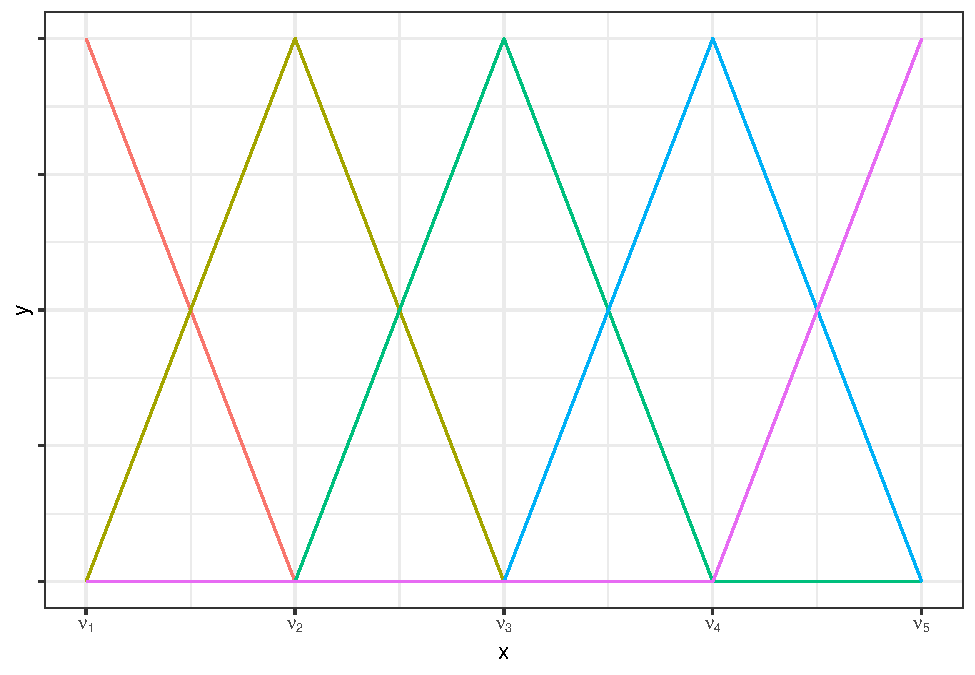
\includegraphics[width=0.32\linewidth]{_main_files/figure-latex/b-splines-plot-1} }\subfloat[degree $2$\label{fig:b-splines-plot-2}]{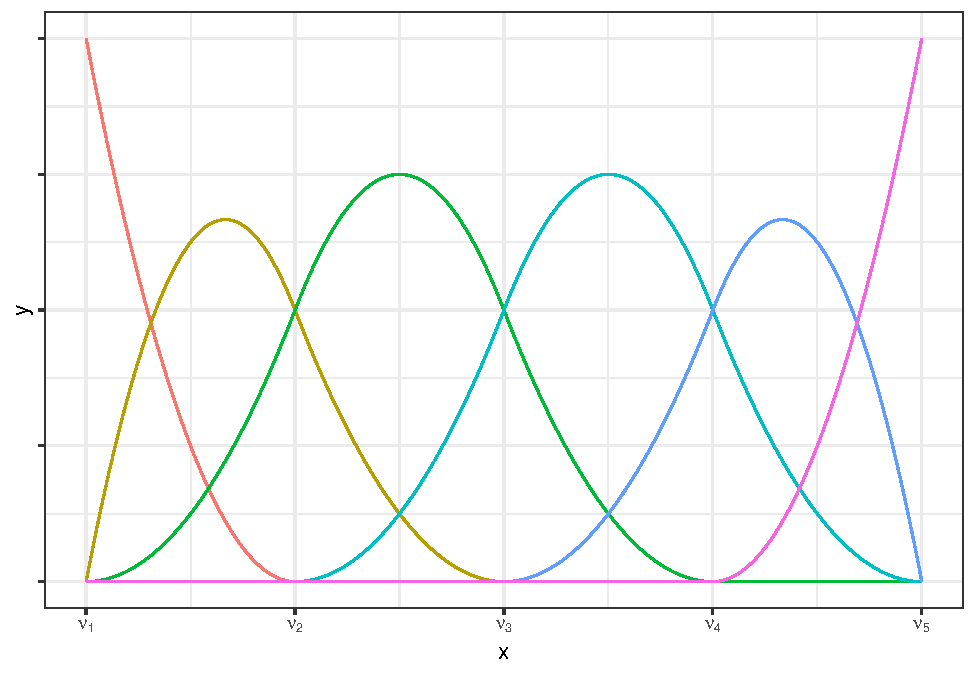
\includegraphics[width=0.32\linewidth]{_main_files/figure-latex/b-splines-plot-2} }\subfloat[degree $3$\label{fig:b-splines-plot-3}]{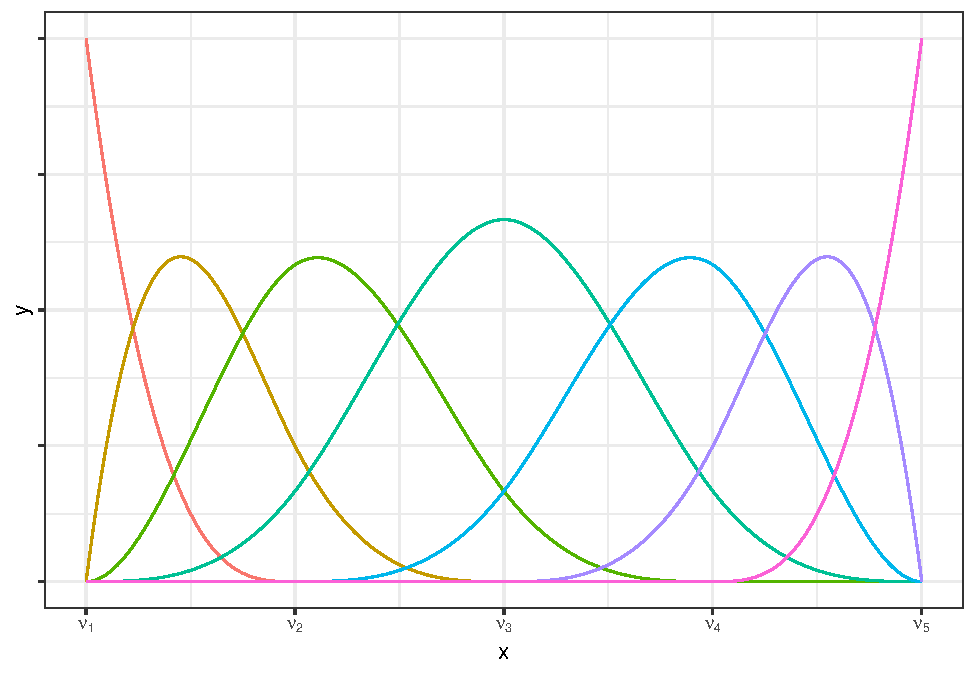
\includegraphics[width=0.32\linewidth]{_main_files/figure-latex/b-splines-plot-3} }

}

\caption{B-splines with different degrees.}\label{fig:b-splines-plot}
\end{figure}

It can be proven that \ref{def:b-splines} defines functions \(B_{j,k}(x)\) that, given \(j\), are splines of degree \(j\). Moreover, \(B_{j,1}, \dots, B_{j,m+j-1}\) constitute a basis of the vector space of the splines of degree \(j\) on the knots \(\nu_1, \dots, \nu_m\). In particular, \(B_{3,1}, \dots, B_{j,m+2}\) constitute a basis of the vector space of the splines of degree \(3\). Therefore, if \(s(x)\) is third degree spline on the knots \(\nu_1, \dots, \nu_m\), it can be expressed as a linear combination of \(B_{3,1}, \dots, B_{3,m+2}\):
\[
s(x) = \sum_{k=1}^{m+2}{\beta_{k}B_{3,k}(x)}
\]

B-splines are preferred compared to truncated polynomial as they are less correlated and lead to more stable and less computationally expensive estimates.

\hypertarget{gam-extensions}{%
\subsubsection{GAM extensions}\label{gam-extensions}}

As in GLM, in GAM we can consider interactions between a variable with non-linear effect \(x_{l_2}\) and another variable \(x_{l_1}\). This can be achieved by adding to the linear predictor a term such as:
\[
x_{l_1} f(x_{l_2})
\]
This is particularly useful when \(x_{l_1}\) is a binary variable and we want to fit two different curves for \(x_{l_2}\) in the case \(x_{l_1}=0\) and in the case \(x_{l_1}=1\).

If we want to consider a more complex interaction between two quantitative variables with non-linear effect, GAM can be extended by considering non-parametrical interactions and modeling them with two-dimensional splines, such as:
\[
f(x_{l_1}, x_{l_2})
\]
In this case, instead of fitting a curve on \((x_l, y)\), we will fit a flexible surface on \((x_{l_1}, x_{l_2}, y)\). This approach can be adopted also for modeling geographical data, in which \(x_{l_1}, x_{l_2}\) are coordinates on the map, such as longitude and latitude.

\hypertarget{some-considerations-on-gam}{%
\subsubsection{Some considerations on GAM}\label{some-considerations-on-gam}}

As we have seen in this chapter, GAMs are flexible tools for fitting quantitative variables with non-linear effects.

One big advantage of GAM is that they are based on the same assumptions of GLM, except for the non-linearity of the components \(f(x_{l})\). The connection with GLM leads to highly interpretable results. Indeed, as we do in GLM, in GAM we can easily observe the marginal effect of a variable \(x_l\) on the response \(y\) just by plotting the graph \(\left(x_l, f(x_l)\right)\), while the interactions between variables are added manually so we have a full control of them.

Another big advantage is that GAM not only provides a flexible tool that produces interpretable results, but this tool works almost automatically. Indeed, while in GLM, when we have to fit a non-linear effect to a quantitative variable \(x_l\), we have to perform a manual process of wise splitting and polynomial fitting on the range of \(x_l\), in GAM we do not have to explicitly specify the shape of \(f(x_l)\) and everything is done by the algorithm.

This higher flexibility and automation comes at the cost of introducing more complexity in the model. Indeed, in a GAM there are much more parameters than in a GLM and this leads to a more computationally expensive fitting. Anyway, this higher complexity produces an higher machine time but significantly reduces the human time that in GLM would be needed for manual fitting.

\newpage

\hypertarget{shrinkage-estimators-for-glm}{%
\subsection{Shrinkage estimators for GLM}\label{shrinkage-estimators-for-glm}}

In this section we are going to present the shrinkage estimators, that are a class of estimators particularly useful in GLM when there are many explanatory variables. All the models presented in this chapter are actually GLM. The advancements consist in the way the parameters are estimated.

\hypertarget{the-bias-variance-trade-off}{%
\subsubsection{The Bias-Variance Trade Off}\label{the-bias-variance-trade-off}}

One of the property of GLM with linear link and Normal response is that the maximum likelihood estimator \(\boldsymbol{\tilde{\beta}}^{ML}\) is unbiased, that is \(E\left(\boldsymbol{\tilde{\beta}}^{ML}\right) = \boldsymbol{\beta}\).\footnote{This property in general is not true for GLM with other links and response distributions, but it is true asymptotically: \(\boldsymbol{\tilde{\beta}}^{ML} \xrightarrow{n\to+\infty} \boldsymbol{\beta}\).} However, the bias is not the only relevant aspect of an estimator. If we consider the \emph{Mean Squared Error} (MSE) of an estimator \(\tilde{\beta}_j\), we get the following result:
\begin{equation}
\label{eq:bias-variance}
MSE\left(\tilde{\beta}_j\right) \eqdef E\left(\left(\tilde{\beta}_j - \beta_j\right)^2\right) =
\underbrace{\left( E(\tilde{\beta}_j)-\beta_j \right)^2}_{\text{Bias}^2} + 
\underbrace{Var\left( \tilde{\beta}_j \right)}_{\text{Variance}}
\end{equation}

The idea behind shrinkage estimators is to add an amount of smart bias to \(\tilde{\beta}_j\) in order to reduce its variance.

The trade-off between Bias and Variance described by equation \eqref{eq:bias-variance} can be interpreted in relation to the complexity of the model. Figure \ref{fig:bias-variance} shows how the prediction error changes by increasing the complexity of the model. In linear smoothers, the complexity of the model can be measured as the effective degrees of freedom \(\text{tr}(H)\) (see section \ref{chap:gam-choice-lambda}), that in the case of the GLM with maximum likelihood estimators is just the number of parameters \(p+1\). Usually, in machine learning models, the complexity of the model is determined by tuning one or more hyper-parameters. In the case of GAM, for example, by increasing \(\lambda\) we obtain a less complex model, while by decreasing it we obtain a more complex model.

A model not complex enough produces estimators with low variance but high bias, that leads to underfitting. A too complex model produces estimators with low bias but high variance, that leads to overfitting.

As with maximum likelihood estimators for GLM the complexity increases with \(p\), they are not suitable when \(p\) is large (high dimensionality).





\begin{figure}[!hbtp]

{\centering 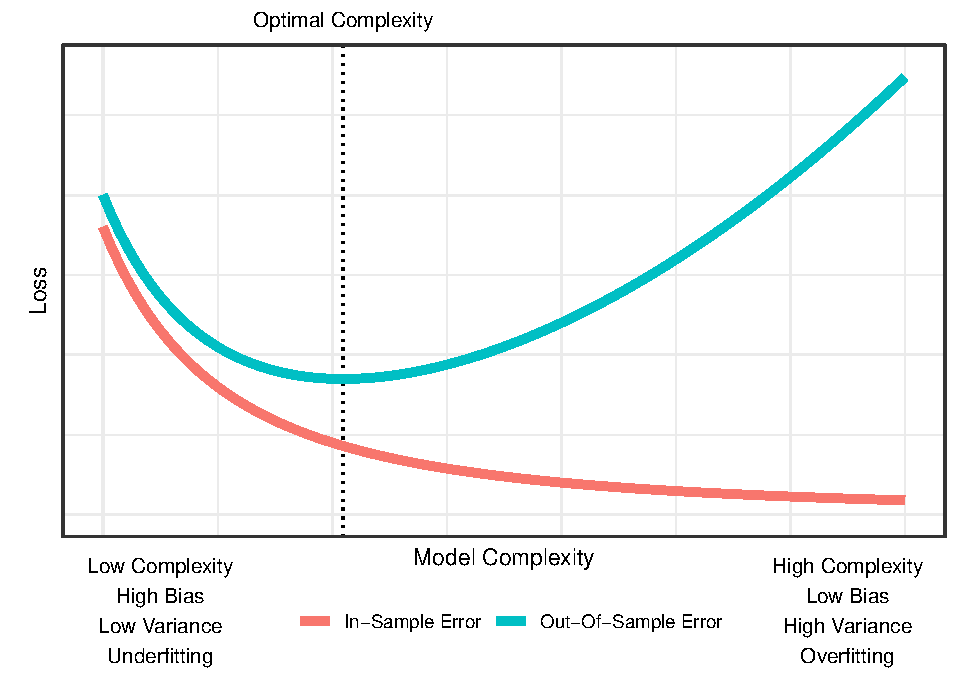
\includegraphics[width=0.8\linewidth]{_main_files/figure-latex/bias-variance-1} 

}

\caption[The Bias-Variance trade off.]{The Bias-Variance trade off. The horizontal axis shows the increase in complexity and the vertical axis shows the effect on in-sample error (training set) and out-of-sample error (test set). The error can be measured as the Mean Squared Error (MSE) or in general as the Deviance.}\label{fig:bias-variance}
\end{figure}

\hypertarget{ridge-regression}{%
\subsubsection{Ridge Regression}\label{ridge-regression}}

One shrinkage estimator for GLM is the \emph{Ridge Regression}. In Ridge Regression, the decrease in variance of \(\tilde{\boldsymbol{\beta}}\) is achieved by considering the optimization problem \eqref{eq:max-lik-est-deviance} and adding to the Deviance a penalization term that depends on the magnitude of \(\beta_1, \beta_2, \dots, \beta_p\):
\begin{equation}
\label{eq:ridge-est-deviance}
\hat{\boldsymbol{\beta}} = \argmin_{\boldsymbol{\beta}\in\mathbb{R}^{p+1}}{\left\{D(\boldsymbol{\beta}, \boldsymbol{y}) + \lambda \|\boldsymbol{\beta}_{\setminus0}\|_2^2\right\}}
\end{equation}
where:

\begin{itemize}
\tightlist
\item
  \(\boldsymbol{\beta}_{\setminus0} = \left(\beta_1, \beta_2, \dots, \beta_p\right)\) is the set of the GLM coefficients except for the intercept \(\beta_0\);
\item
  \(\|\cdot\|_2^2\) is the \(L^2\) norm, i.e.~\(\|\boldsymbol{\beta}_{\setminus0}\|_2^2 = \sum_{j=1}^p{\beta_j^2}\);
\item
  \(\lambda\ge0\) is an hyper-parameter that controls the penalization.
\end{itemize}

The term \(\|\boldsymbol{\beta}_{\setminus0}\|_2^2\) produces a penalization for high values of \(\beta_j\). This penalization leads to a shrinkage of the coefficients.
The exclusion of \(\beta_0\) from the penalization term is intended to prevent the introduction of a bias towards \(0\) in the intercept. As the magnitude of \(\beta_j\) depends on the values of \(x_j\), it is preferred to standardize all the explanatory variables to avoid distorting effects due to the unit of measure of the explanatory variables.

As for GAM, the hyper-parameter \(\lambda\) determines the amount of penalization given to high values of the coefficients \(\hat{\beta}_j\). If \(\lambda=0\), the optimization problem \eqref{eq:ridge-est-deviance} corresponds to the maximum likelihood. As \(\lambda\) increases, the optimal coefficients \(\hat{\beta}_j\) tends to shrink towards \(0\). In the limit case, if \(\lambda\to+\infty\), the optimal coefficients \(\hat{\beta}_j\) are all equal to \(0\), except for \(\hat{\beta}_0\), that is equal to \(\bar{y}\), so the estimated model corresponds to the trivial model with only the intercept \(g(\mu)=\beta_0\).

An example of the effect of \(\lambda\) is reported in figure \ref{fig:ridge-lambda}. The data represented has been simulated from a GLM with idenity link and Normal response. As we can see, if \(\lambda=0\), all the estimated responses \(\hat{\mu}_j\) correspond to the average of the response on that group \(\bar{y}_j\). As \(\lambda\) increases, the estimated responses move towards the global average \(\bar{y}\). The speed of convergence to \(0\) depends on how much the group average \(\bar{y}_j\) differs from the global average \(\bar{y}\) and on the number of observation of the group: if in a group \(j\) there are many observations, we have a lot of information on that group, the group average \(\bar{y}_j\) have a small variance and it is a reliable estimate for \(\mu_j\), while if there are few observations, the group average \(\bar{y}_j\) have a high variance and it is not very reliable.

The optimal point for \(\lambda=0\) can be obtained through a Cross Validation as seen in section \ref{chap:gam-choice-lambda}.







\begin{figure}[!hbtp]

{\centering \subfloat[$\lambda = 0$\label{fig:ridge-lambda-1}]{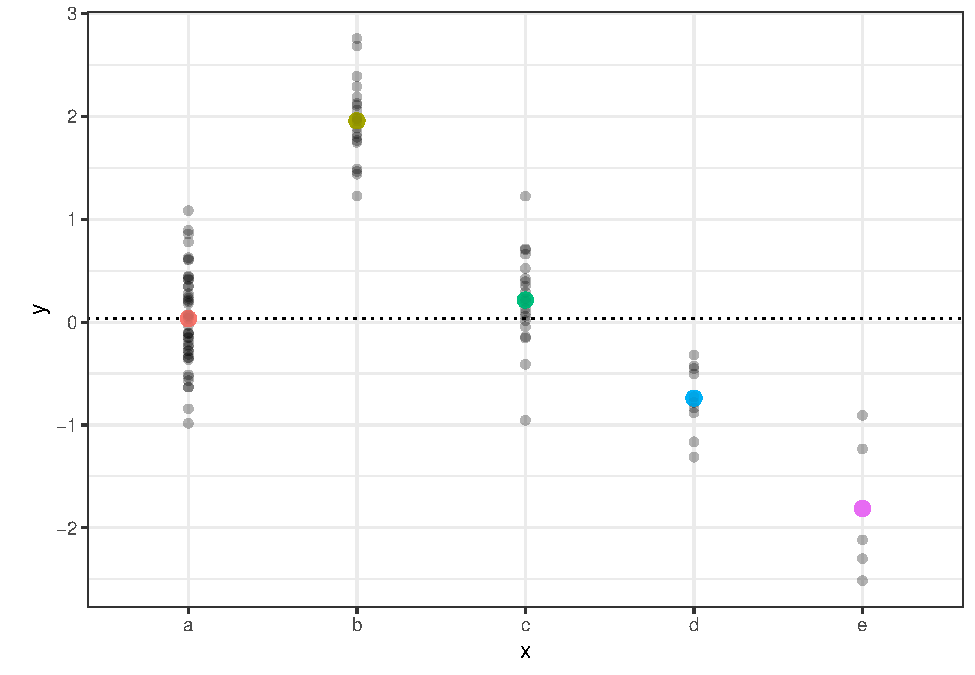
\includegraphics[width=0.5\linewidth]{_main_files/figure-latex/ridge-lambda-1} }\subfloat[$\lambda = 0.1$\label{fig:ridge-lambda-2}]{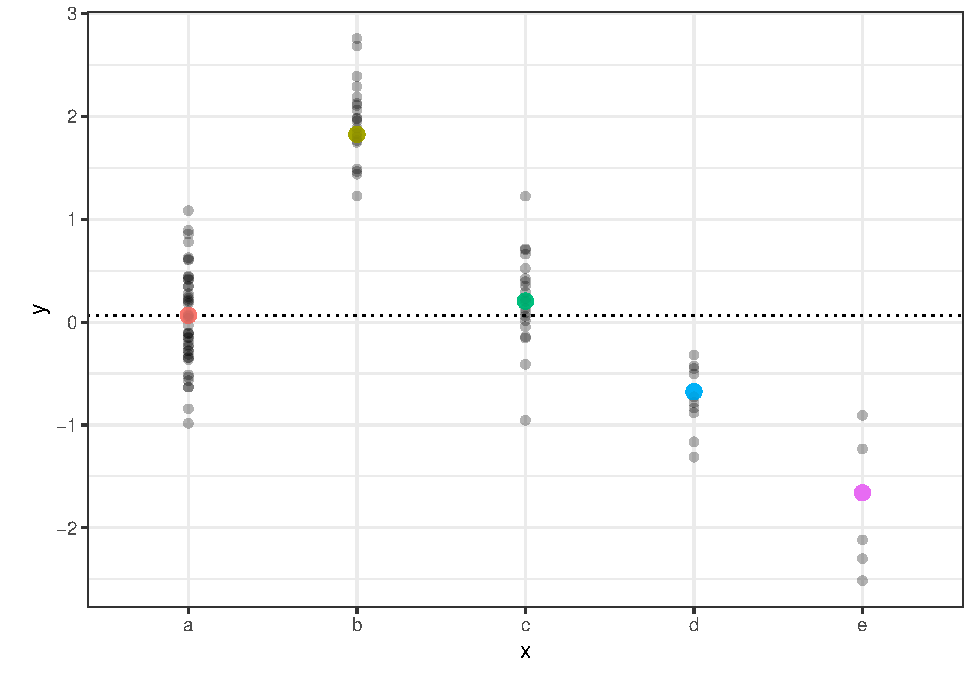
\includegraphics[width=0.5\linewidth]{_main_files/figure-latex/ridge-lambda-2} }\newline\subfloat[$\lambda = 1$\label{fig:ridge-lambda-3}]{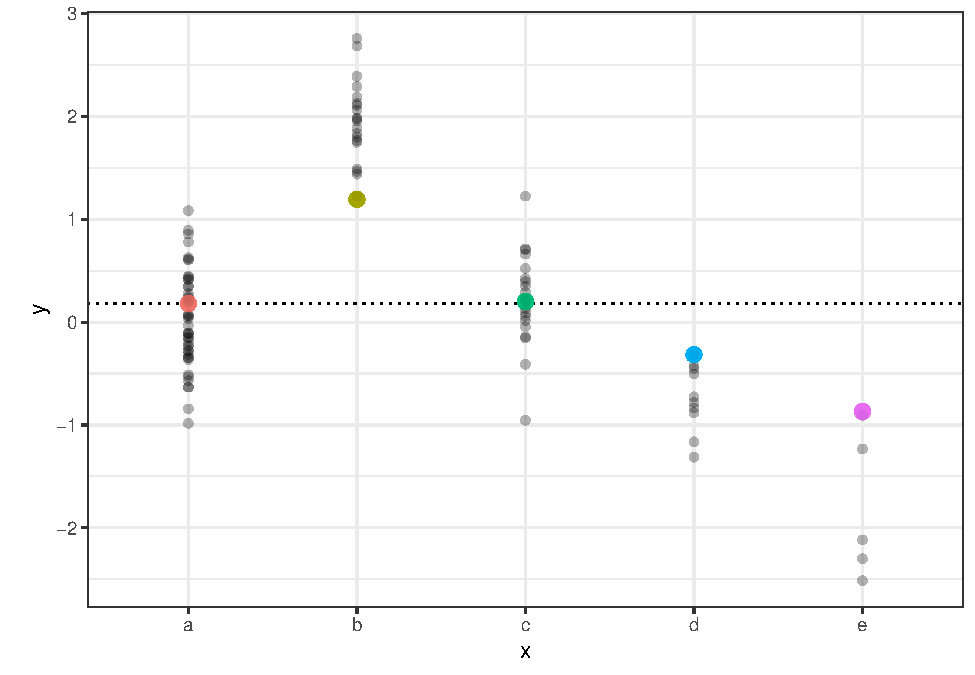
\includegraphics[width=0.5\linewidth]{_main_files/figure-latex/ridge-lambda-3} }\subfloat[$\lambda = 10$\label{fig:ridge-lambda-4}]{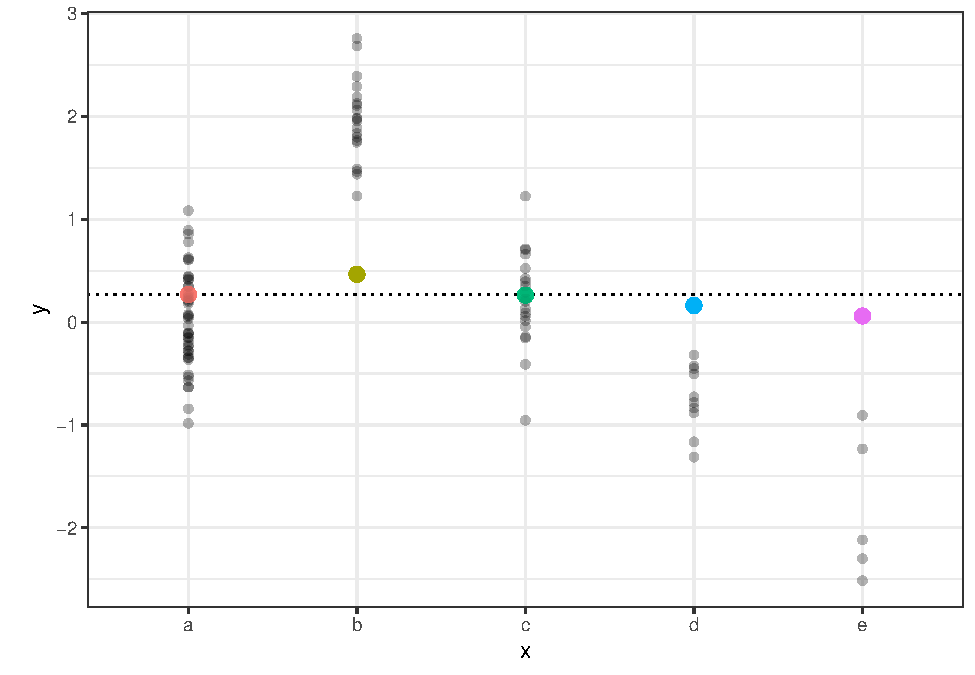
\includegraphics[width=0.5\linewidth]{_main_files/figure-latex/ridge-lambda-4} }\newline\subfloat[$\hat{\beta}_j$ for different values of $\lambda$\label{fig:ridge-lambda-5}]{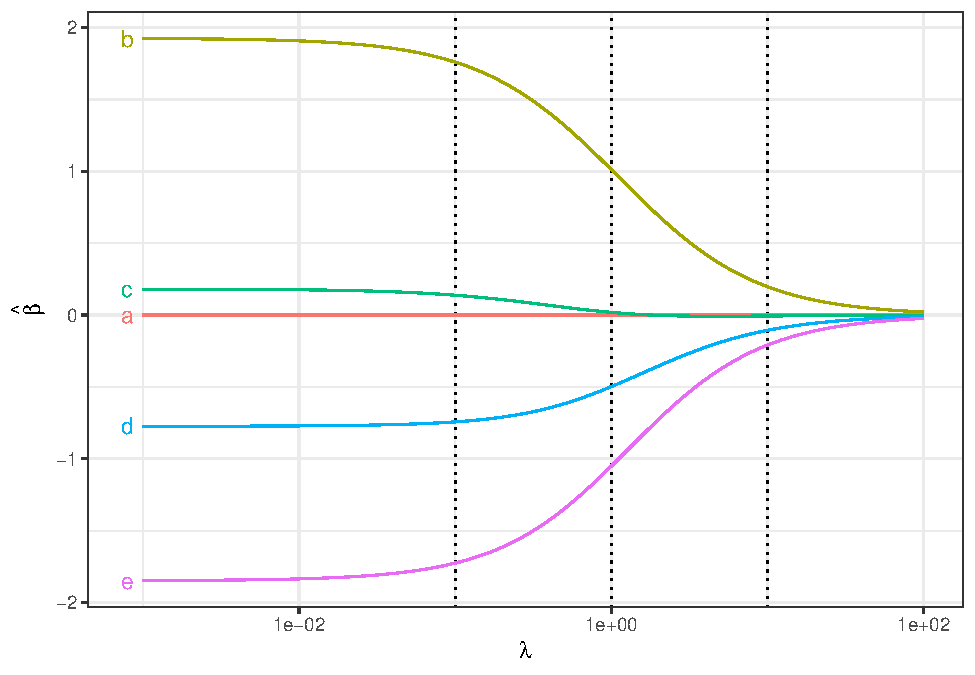
\includegraphics[width=0.7\linewidth]{_main_files/figure-latex/ridge-lambda-5} }

}

\caption[The Bias-Variance trade off. Ridge Regression coefficients for different levels of the penalization parameter \(\lambda\).]{Ridge Regression coefficients for different levels of the penalization parameter \(\lambda\). If \(\lambda=0\), the coefficients correspond to the maximum likelihood coefficients. As \(\lambda\) increases, the coefficients are shrunk towards \(0\).}\label{fig:ridge-lambda}
\end{figure}

The case of GLM with identity link and Normal distribution is particularly convenient for the interpretation, because, in this case, the optimization problem \eqref{eq:ridge-est-deviance} has an explicit solution. To make the results more interpretable, let's assume that the response variables have \(E(Y)=0\) and that the explanatory variables are centered on \(0\), i.e.~\(\bar{x}_j=0, \ j\in\{1,2,\dots,p\}\). That means that \(\beta_0=0\) and the model is \(E(Y)=\beta_1x_1+\beta_2x_2+\dots+\beta_px_p\). With these assumptions, we obtain:
\begin{equation}
\label{eq:ridge-estimator}
\hat{\boldsymbol{\beta}}_{\lambda,\setminus0} = \left(\boldsymbol{X}^t\boldsymbol{X}+\lambda I_p\right)^{-1}\boldsymbol{X}^t y
\end{equation}
where:

\begin{itemize}
\tightlist
\item
  \(\hat{\boldsymbol{\beta}}_{\lambda,\setminus0} = \left(\hat{\beta}_1, \hat{\beta}_2, \dots, \hat{\beta}_p\right)\);
\item
  \(\boldsymbol{X}\) is the design matrix without the first column of \(1\)s, as the intercept is excluded from the model;
\item
  \(I_p\) is the identity matrix with dimension \(p\).
\end{itemize}

From the formula \eqref{eq:ridge-estimator} we can see that, while the maximum likelihood estimator is unbiased, if \(\lambda>0\) the Ridge estimator is biased.
\begin{align*}
E\left(\tilde{\boldsymbol{\beta}}_{0,\setminus0}\right) & =
\left(\boldsymbol{X}^t\boldsymbol{X}\right)^{-1}\boldsymbol{X}^t E(Y) \\ & =
\left(\boldsymbol{X}^t\boldsymbol{X}\right)^{-1}\boldsymbol{X}^t \boldsymbol{X} \boldsymbol{\beta}_{\setminus0} \\ & =
\boldsymbol{\beta}_{\setminus0} \\[6pt]
E\left(\tilde{\boldsymbol{\beta}}_{\lambda,\setminus0}\right) & =
\left(\boldsymbol{X}^t\boldsymbol{X}+\lambda I_p\right)^{-1}\boldsymbol{X}^t E(Y) \\ & =
\left(\boldsymbol{X}^t\boldsymbol{X}+\lambda I_p\right)^{-1}\boldsymbol{X}^t\boldsymbol{X} \boldsymbol{\beta}_{\setminus0} \\ & \neq
\boldsymbol{\beta}_{\setminus0}
\end{align*}

Moreover, from the formula \eqref{eq:ridge-estimator} we find that, even if there is multicollinearity and \(\boldsymbol{X}^t\boldsymbol{X}\) is not invertible, the Ridge estimator is computable. This aspect is particularly interesting when \(p > n\).

If we assume that the explanatory variables are independent and standardized, i.e.~\(\boldsymbol{X}^t\boldsymbol{X} = I_p\), we can further simplify the expression \eqref{eq:ridge-estimator} to:
\[
\hat{\boldsymbol{\beta}}_{\lambda,\setminus0} =
\frac{1}{1+\lambda} \boldsymbol{X}^t y = 
\frac{1}{1+\lambda} \hat{\boldsymbol{\beta}}_{0,\setminus0}
\]
that results in:
\begin{align*}
E\left(\tilde{\boldsymbol{\beta}}_{\lambda,\setminus0}\right) & =
\frac{1}{1+\lambda} \boldsymbol{\beta}_{\setminus0} \\
Var\left(\tilde{\boldsymbol{\beta}}_{\lambda,\setminus0} \right) & =
\frac{1}{\left(1+\lambda\right)^2} Var\left( \tilde{\boldsymbol{\beta}}_{0,\setminus0} \right)
\end{align*}

This result means that, if the explanatory variables are independent, the Ridge penalization shrinks all the estimated coefficients by a factor of \(\frac{1}{1+\lambda}\) and reduce their variance by a factor of \(\frac{1}{\left(1+\lambda\right)^2}\).

From formula \eqref{eq:ridge-estimator} we also find that, as in GAM, if the link is identity and the response is Normal, the Ridge regression is a linear smoother. In this case the smoothing matrix is:
\[
H_{\lambda} = \boldsymbol{X} \left(\boldsymbol{X}^t\boldsymbol{X}+\lambda I_p\right)^{-1}\boldsymbol{X}^t
\]

In the case of independent explanatory variables we get:
\[
H_{\lambda} = \frac{1}{1+\lambda} \boldsymbol{X} \boldsymbol{X}^t = \frac{1}{1+\lambda} H_0
\]
and then \(\text{tr}\left(H_{\lambda}\right) = \frac{p}{1+\lambda}\). This result means that, by increasing \(\lambda\), the effective number of degrees of fredom decreases.

\hypertarget{lasso-regression}{%
\subsubsection{LASSO Regression}\label{lasso-regression}}

Another shrinkage estimator for GLM is the \emph{LASSO} (Least Absolute Shrinkage and Selection Operator). LASSO is based on the same idea of Ridge Regression, but, instead of considering a penalization based on \(L^2\) norm, it considers a penalization based on \(L^1\) norm:
\begin{equation}
\label{eq:lasso-est-deviance}
\hat{\boldsymbol{\beta}} = \argmin_{\boldsymbol{\beta}\in\mathbb{R}^{p+1}}{\left\{D(\boldsymbol{\beta}, \boldsymbol{y}) + \lambda \|\boldsymbol{\beta}_{\setminus0}\|_1\right\}}
\end{equation}
where:

\begin{itemize}
\tightlist
\item
  \(\boldsymbol{\beta}_{\setminus0} = \left(\beta_1, \beta_2, \dots, \beta_p\right)\) is the set of the GLM coefficients except for the intercept \(\beta_0\);
\item
  \(\|\cdot\|_1\) is the \(L^1\) norm, i.e.~\(\|\boldsymbol{\beta}_{\setminus0}\|_1 = \sum_{j=1}^p{|\beta_j|}\);
\item
  \(\lambda\ge0\) is an hyper-parameter that controls the penalization.
\end{itemize}

An example of the effect of the \(L^1\) penalization for different values of \(\lambda\) is shown in figure \ref{fig:lasso-lambda}. The simulated dataset is the same used for the Ridge example in figure \ref{fig:ridge-lambda}. As we can see from the plots, the substantial difference between Ridge and LASSO is that in LASSO from a certain value of \(\lambda\) the coefficients are shrunk exactly to \(0\). While in Ridge that is just a limit property, in LASSO, for each coefficient \(\beta_j\) there is a level of the penalization parameter \(\lambda'_j\) such that for \(\lambda \ge \lambda'_j\), the estimated coefficient \(\hat{\beta}_j\) is forced to exactly \(0\).







\begin{figure}[!hbtp]

{\centering \subfloat[$\lambda = 0$\label{fig:lasso-lambda-1}]{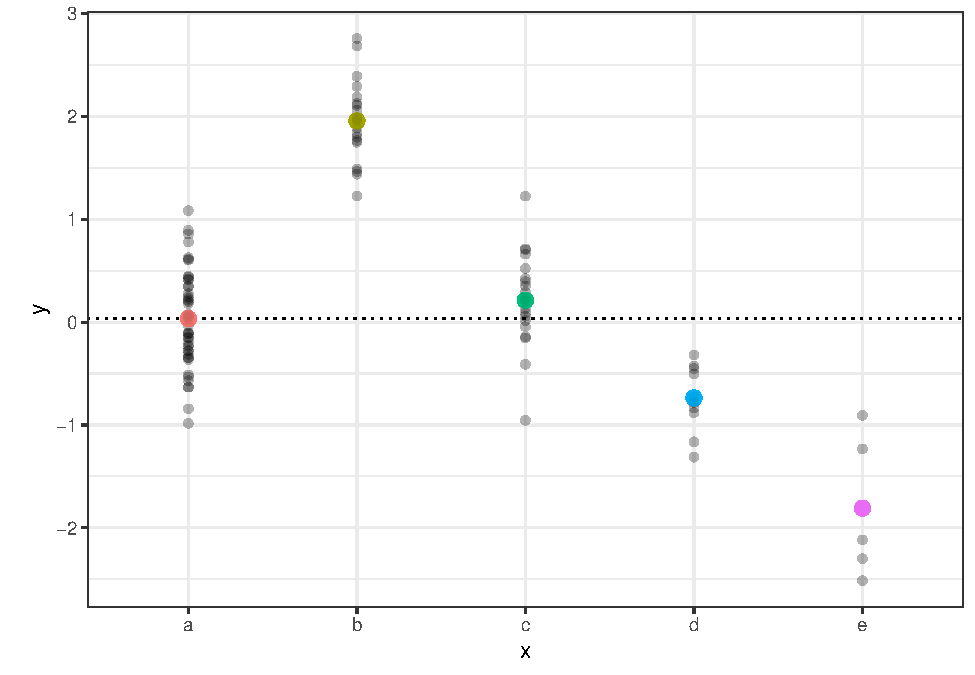
\includegraphics[width=0.5\linewidth]{_main_files/figure-latex/lasso-lambda-1} }\subfloat[$\lambda = 0.1$\label{fig:lasso-lambda-2}]{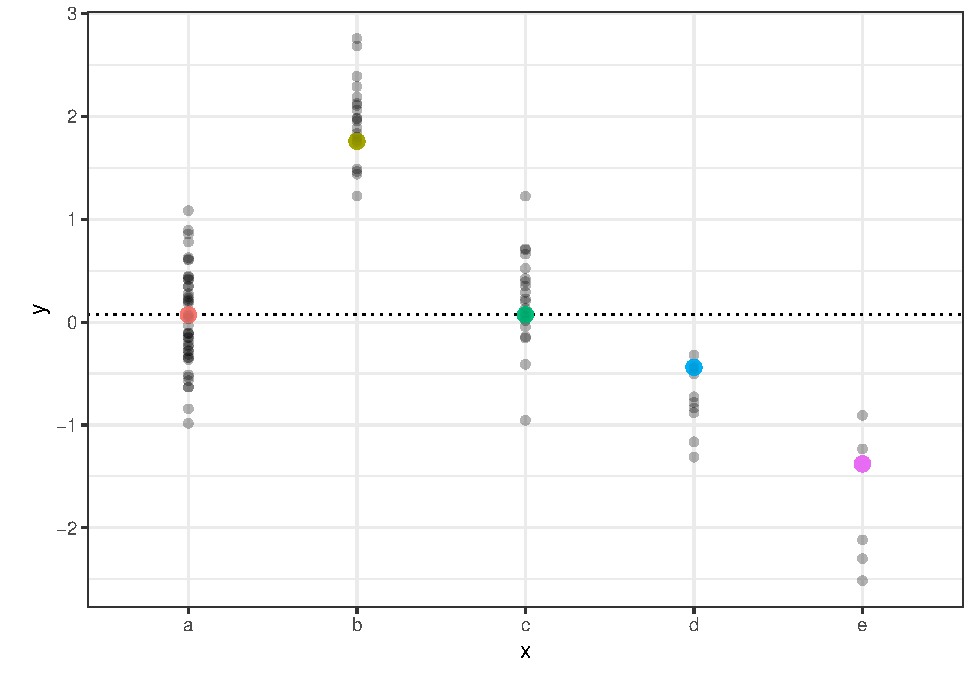
\includegraphics[width=0.5\linewidth]{_main_files/figure-latex/lasso-lambda-2} }\newline\subfloat[$\lambda = 0.6$\label{fig:lasso-lambda-3}]{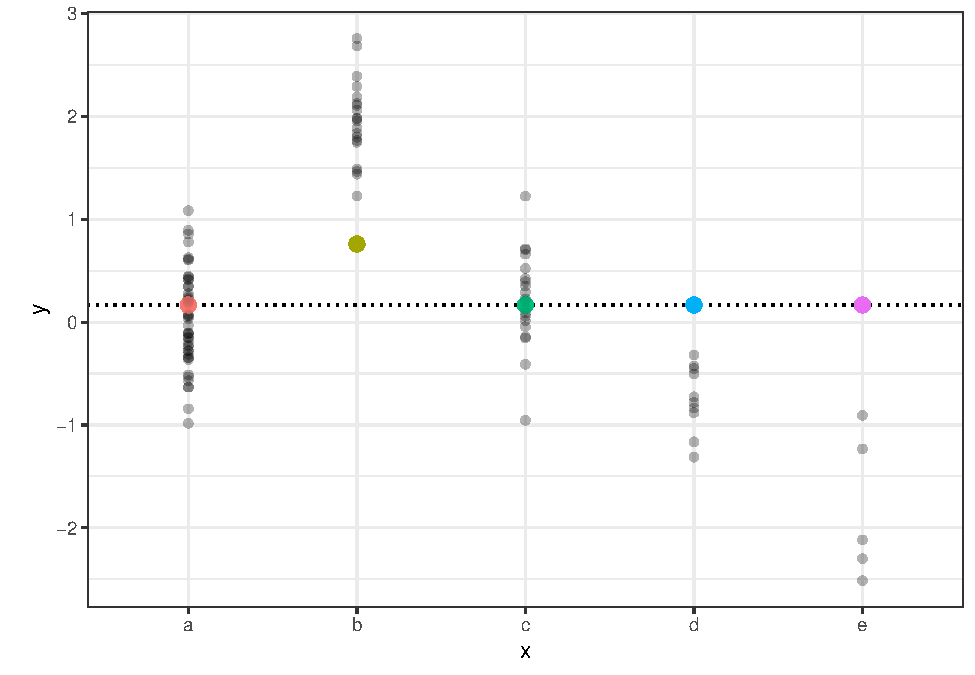
\includegraphics[width=0.5\linewidth]{_main_files/figure-latex/lasso-lambda-3} }\subfloat[$\lambda = 1$\label{fig:lasso-lambda-4}]{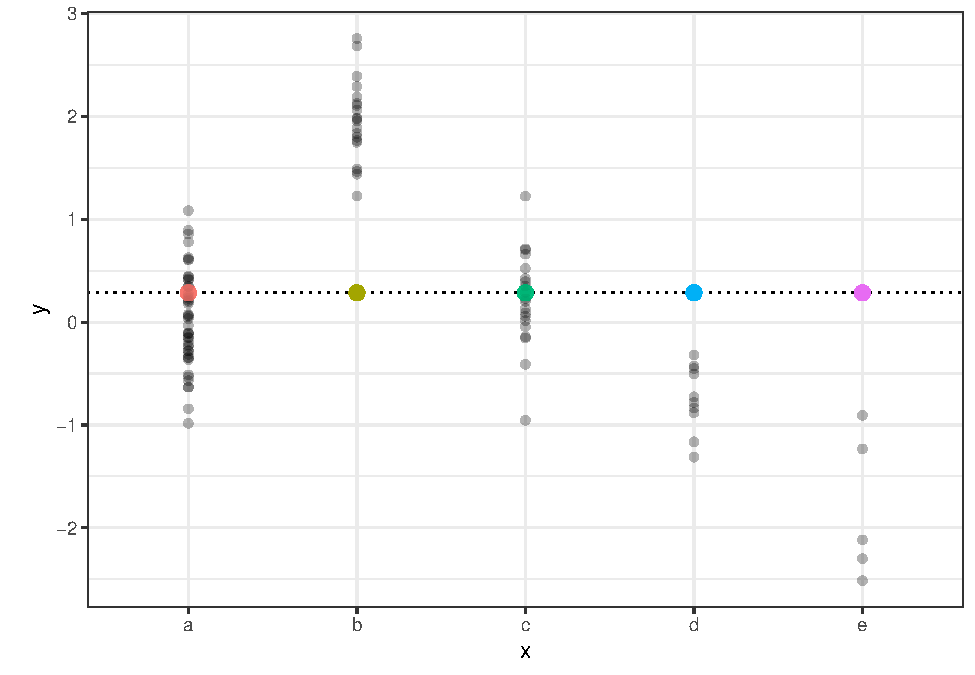
\includegraphics[width=0.5\linewidth]{_main_files/figure-latex/lasso-lambda-4} }\newline\subfloat[$\hat{\beta}_j$ for different values of $\lambda$\label{fig:lasso-lambda-5}]{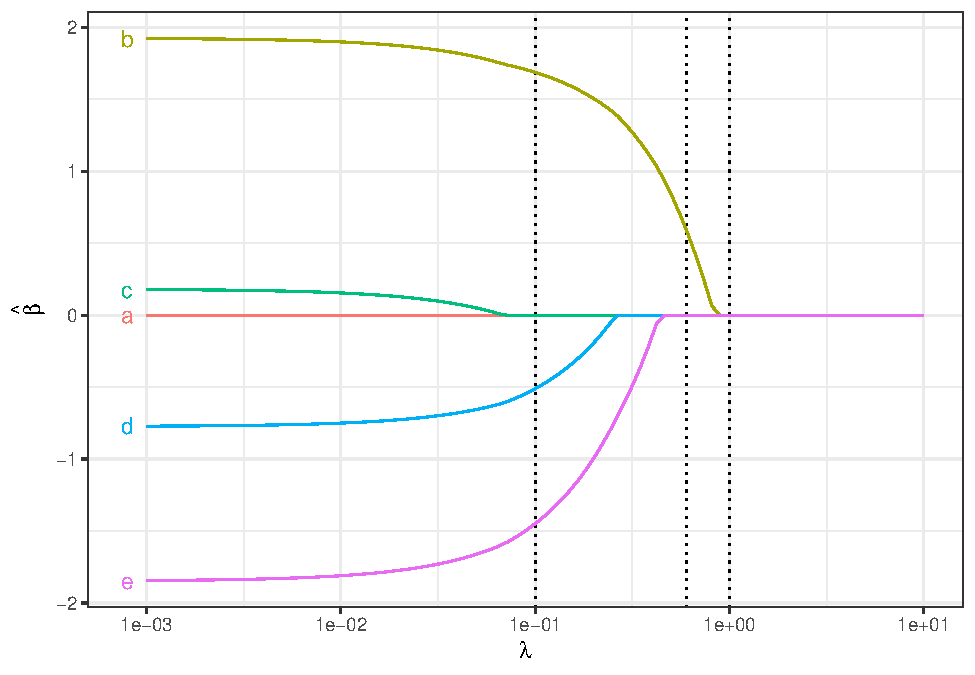
\includegraphics[width=0.7\linewidth]{_main_files/figure-latex/lasso-lambda-5} }

}

\caption[The Bias-Variance trade off. LASSO Regression coefficients for different levels of the penalization parameter \(\lambda\).]{LASSO Regression coefficients for different levels of the penalization parameter \(\lambda\). If \(\lambda=0\), the coefficients correspond to the maximum likelihood coefficients. As \(\lambda\) increases, the coefficients are shrunk towards \(0\). High values of \(\lambda\) force the coefficients to be exactly equal to \(0\).}\label{fig:lasso-lambda}
\end{figure}

This property of the LASSO Regression can be derived from a different representation of the optimization problems \eqref{eq:ridge-est-deviance} and \eqref{eq:lasso-est-deviance}. It can be proven that in general, considering a penalization given by the \(L^d\) norm, the unconstrained optimization problem:
\begin{equation}
\label{eq:ld-est-deviance}
\hat{\boldsymbol{\beta}} = \argmin_{\boldsymbol{\beta}\in\mathbb{R}^{p+1}}{\left\{D(\boldsymbol{\beta}, \boldsymbol{y}) + \lambda \|\boldsymbol{\beta}_{\setminus0}\|_d^d\right\}}
\end{equation}
is equivalent to the constrained optimization problem:
\begin{equation}
\label{eq:lp-est-deviance-constr}
\hat{\boldsymbol{\beta}} = \argmin_{\boldsymbol{\beta}\in\mathbb{R}^{p+1}:\  \|\boldsymbol{\beta}_{\setminus0}\|_d^d \le s_{\lambda}}{ D(\boldsymbol{\beta}, \boldsymbol{y}) }
\end{equation}
where \(s_{\lambda}\) is a quantity that depends on \(\lambda\).

The representation \eqref{eq:lp-est-deviance-constr} provides a useful geometric interpretation of the optimization problem. Figure \ref{fig:opt-ridge-lasso} shows the visual representation of the optimization problem \eqref{eq:lp-est-deviance-constr} in the Ridge case (\(d=2\)) and in the LASSO case (\(d=1\)). The axes represent the component of \(\boldsymbol{\beta}\). The point \(\hat{\boldsymbol{\beta}}^{ML}\) represents the maximum likelihood estimator for \(\boldsymbol{\beta}\), that is the optimal point for the Deviance \(D(\boldsymbol{\beta}, \boldsymbol{y})\) without any constraints. The ellipses around \(\hat{\boldsymbol{\beta}}^{ML}\) represent the contour lines of \(D(\boldsymbol{\beta}, \boldsymbol{y})\). In the Normal case with identity link they are concentric ellipses centered in \(\hat{\boldsymbol{\beta}}^{ML}\). The grey area around the axes intersection represents the feasibility region determined by \(\|\boldsymbol{\beta}\|_d^d \le s_\lambda\). This area, in the Ridge case corresponds to the circle \(\|\boldsymbol{\beta}\|_2^2 \le s_\lambda\), while in the LASSO case corresponds to the square \(\|\boldsymbol{\beta}\|_1^1 \le s_\lambda\). The sharpness of the LASSO feasibility region imply that the optimal point \(\hat{\boldsymbol{\beta}}^{LASSO}\) could fall into one of the corners of the square leading one of the coefficients \(\hat{\beta}_j^{LASSO}\) to be exactly equal to \(0\). In general, if there are more than two explanatory variables, the LASSO feasibility region is an hyper-cube and the LASSO attains solutions with many coefficients exactly equal to \(0\).







\begin{figure}[!hbtp]

{\centering \subfloat[Ridge\label{fig:opt-ridge-lasso-1}]{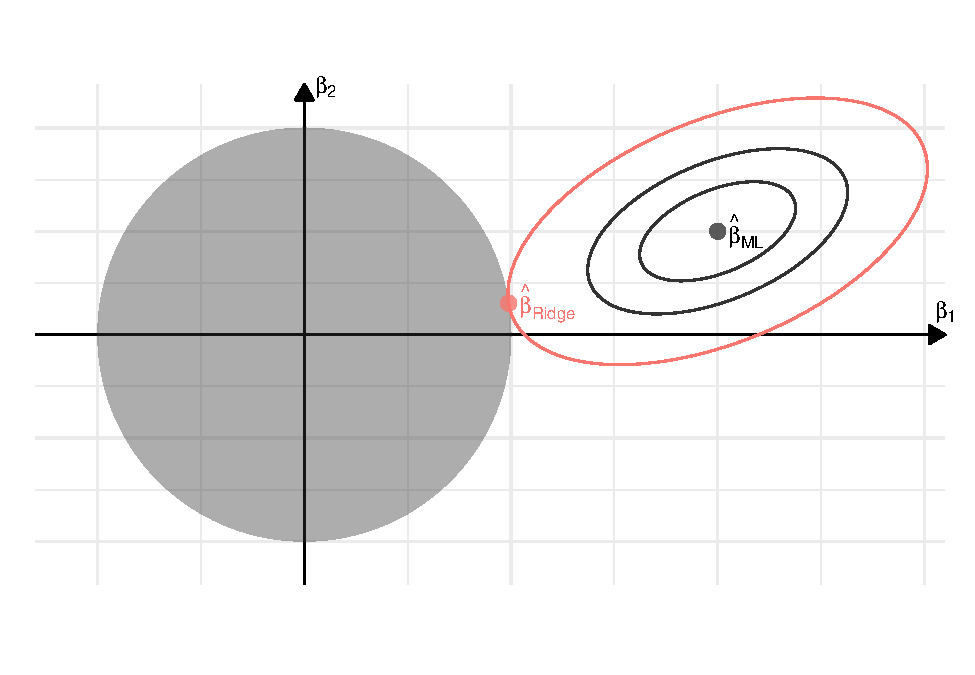
\includegraphics[width=0.5\linewidth]{_main_files/figure-latex/opt-ridge-lasso-1} }\subfloat[LASSO\label{fig:opt-ridge-lasso-2}]{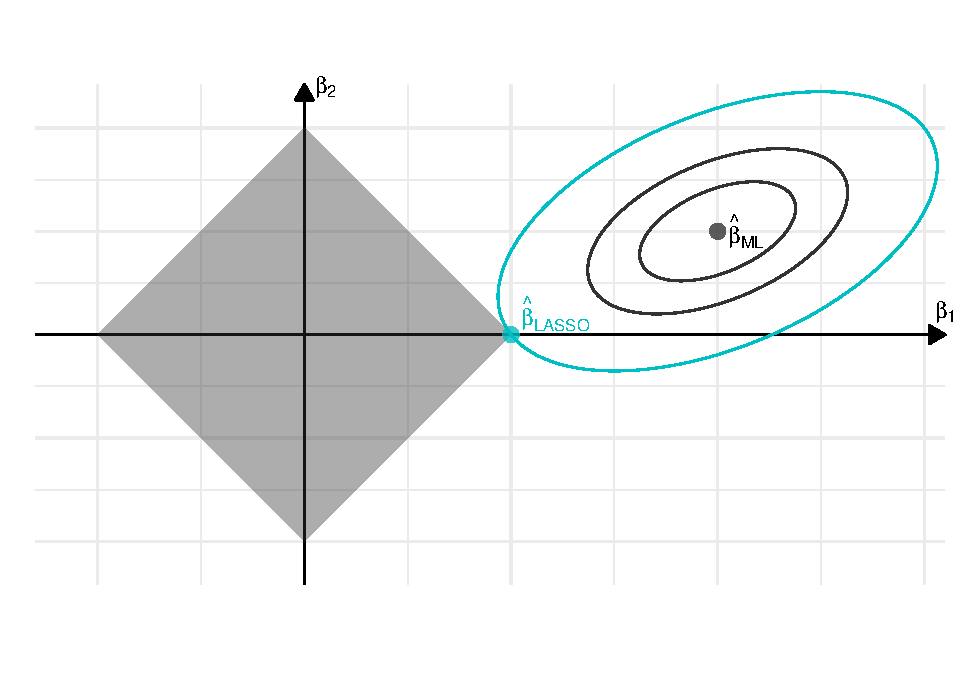
\includegraphics[width=0.5\linewidth]{_main_files/figure-latex/opt-ridge-lasso-2} }

}

\caption[Geometrical interpretation of the optimization problem for Ridge and LASSO.]{Geometrical interpretation of the optimization problem for Ridge and LASSO. The axes represent the components of \(\boldsymbol{\beta}\). The point \(\hat{\boldsymbol{\beta}}^{ML}\) represents the maximum likelihood estimator for \(\boldsymbol{\beta}\), that is the optimal point for the Deviance \(D(\boldsymbol{\beta}, \boldsymbol{y})\) without any constraints. The ellipses around \(\hat{\boldsymbol{\beta}}^{ML}\) represent the contour lines of \(D(\boldsymbol{\beta}, \boldsymbol{y})\). The grey area around the axes intersection represents the feasibility region determined by \(\|\boldsymbol{\beta}\|_d^d \le s_\lambda\), that is a circle in the Ridge case \(\|\boldsymbol{\beta}\|_2^2 \le s_\lambda\) and a square in the LASSO case \(\|\boldsymbol{\beta}\|_1^1 \le s_\lambda\). \(\hat{\boldsymbol{\beta}}^{Ridge}\) and \(\hat{\boldsymbol{\beta}}^{LASSO}\) are respectively the optimal point conditioned to the Ridge constraint and the optimal point conditioned to the LASSO constraint. The sharpness of the LASSO feasibility region imply that the optimal point \(\hat{\boldsymbol{\beta}}^{LASSO}\) could fall into one of the corners of the square leading one of the coefficients \(\hat{\beta}_j^{LASSO}\) to be exactly equal to \(0\).}\label{fig:opt-ridge-lasso}
\end{figure}

The fact that in LASSO Regression the estimated coefficients can be exactly equal to \(0\) is a precious benefit. Indeed, LASSO Regression performs a feature selection removing the coefficients that are not relevant for predicting the response. The LASSO fitting is much more efficient than the other procedures we have seen for feature selection in GLM such as the stepwise selection based on AIC or other criteria (section \ref{chap:variable-selection}) and it is better scalable for datasets with many variables. It is also possible to use the variables selected by the LASSO regression and giving them as input for a maximum likelihood fitting. If in the dataset there are many variable but only few of them are relevant for the response, this procedure can returns better predictions than just LASSO regression.

\hypertarget{elastic-net}{%
\subsubsection{Elastic Net}\label{elastic-net}}

Compared to the Ridge Regression, the LASSO Regression has the benefit of performing a feature selection by forcing many coefficients to \(0\). Anyway this doesn't necessarily mean that the LASSO produces estimates that always outperform Ridge estimates. It strongly depends on the case. In general, if in a dataset only few of the explanatory variables have an effect on the response, the LASSO will produce better estimates, but, if all the variables bring a small amount of information on the response, the the LASSO will suppress some of this information, while the Ridge will catch it. The problem is that in practice, when we have a real dataset, we do not know in which case we are. The \emph{Elastic Net} is a generalization of the Ridge and the LASSO that provides a solution for this kind of problem.

The Elastic Net consists in a penalized Deviance optimization problem in which the penalization term is a mixture of the Ridge penalization and the LASSO penalization:
\begin{equation}
\label{eq:elastic-net-est-deviance}
\hat{\boldsymbol{\beta}} =  \argmin_{\boldsymbol{\beta}\in\mathbb{R}^{p+1}}{\left\{
D(\boldsymbol{\beta}, \boldsymbol{y}) +
\lambda 
\sum_{j=1}^p{\left(\alpha |\beta_j| + (1 - \alpha) |\beta_j|^2\right)}
\right\}}
\end{equation}
where \(\alpha \in [0,1]\) is an hyper-parameter that weights the two penalization components.

Looking to the equation \eqref{eq:elastic-net-est-deviance} it is clear that, if \(\alpha=0\), the Elastic Net corresponds to the Ridge Regression, while, if \(\alpha=1\), the Elastic Net corresponds to the LASSO regression. If \(\alpha \in ]0,1[\), the result will be a compromise between the two.

The hyper-parameter \(\alpha\) can be estimated together with \(\lambda\) in a Cross Validation procedure (see section \ref{chap:variable-selection}). If the data suggests that many variables are useful for predicting the response, the estimated hyper-parameter \(\hat{\alpha}\) will be close to \(0\), while if the data suggests that only few variables are useful, the estimated hyper-parameter \(\hat{\alpha}\) will be close to \(1\).

\hypertarget{chap:shrinkage-considerations}{%
\subsubsection{Some considerations on Shrinkage Estimators}\label{chap:shrinkage-considerations}}

As we have said, shrinkage estimators are particularly useful when the number of parameters \(p\) in the model is large (high dimensionality) and the maximum likelihood estimator have a high variance. This could happen when we have some qualitative variables with many modalities, as for example the make and the model of the insured vehicle in car insurance. As we have seen with the examples represented in figure \ref{fig:ridge-lambda} and \ref{fig:lasso-lambda}, the penalization will shrink more the coefficients in the groups with few observations and only the groups with an average response \(\bar{y}_j\) significantly different from the global average response \(\bar{y}\) will emerge. This procedure is more efficient and more robust to overfitting than grouping modalities based on hypothesis testing or other criteria.

If we are in a case in which we already performed a satisfying feature selection and we only want to shrink some of the coefficients we can apply the penalization only to them. For example, in the case of the variables make and model, we can consider an Elastic Net penalization only to the coefficients \(\beta_j\) corresponding to the modalities of those variables. This technique is useful also in the case we have explanatory variables with distribution highly unbalanced. For example, if we consider the variable ``number of claims experienced in the previous year'', we will have most of the observation in the modality corresponding to \(0\) claims, very few in the modality corresponding to \(1\) claim and almost nobody with \(2\) or more claims. If we are fitting a model for the claim frequency and we consider the variable \(x_j\) that indicates whether the policyholder experienced one or more claims in the previous year \(x_j=1\) or not \(x_j=0\), it is likely that the maximum likelihood estimator for the coefficient \(\hat{\beta}_{x_j=1}\) will be greater than \(0\), as the policyholders that experienced claims are usually more inclined to experience more of them in the future. However, given that in there are just few observation with \(x_j=1\) it is possible that the coefficient \(\hat{\beta}_{x_j=1}\) is not significantly different from \(0\). If our only tool is the maximum likelihood estimator, we have to choose whether to insert the variable \(x_j\) in the model or not. If we don't consider it we are probably discard some potentially useful information, while if we consider it and we estimate its coefficient with maximum likelihood we risk to overfit the data. With shrinkage estimators we can choose to insert the variable \(x_j\) in the model and fitting it with a penalization. This way we exploit that information but we prevent overfitting.

Another interesting observation about GLM fitting is that in the practice, when maximum likelihood estimates are adopted, what is done is not just fitting a model with all the variables, but a feature selection is conducted. The fact that a variable \(x_j\) is inserted in the model depends on whether the feature selection procedure selects that variable or not. That corresponds to estimating the coefficient \(\beta_j\) with an estimator \(\tilde{\beta}_j\) that is equal to the maximum likelihood estimator \(\tilde{\beta}_j^{ML}\) when the coefficient pass a specific criterion and is equal to \(0\) when \(\tilde{\beta}_j^{ML}\) doesn't pass that criterion. This criterion could be something objective as for example the decrease in AIC and the significance in a hypothesis testing on \(\tilde{\beta}_j^{ML}\), and also something more subjective based also on the domain knowledge on the person that is conducting the modeling. Actually, this feature selection procedure introduces a bias towards \(0\) of the coefficient \(\tilde{\beta}_j\) that reduces its variance as all the coefficients not relevant for prediction are set equal to \(0\) and only the relevant ones are fitted with maximum likelihood. If we consider a binary variable \(x_j\), in all the procedures commonly used for feature selection, the probability that \(\tilde{\beta}_j\) passes the procedure or not depends on how strong the effect \(\beta_j\) is and how many observations there are in the classes \(x_j=0\) and \(x_j=1\).

We also mantion that the Shrinkage Estimators can be used in synergy with GAMs. Indeed it is possible to fit to the quantitative variables a cubic spline with a GAM penalization based on the second derivative of the spline and to the qualitative variables a shrinkage estimator with an Elastic Net penalization.
\begin{equation}
\label{eq:gam-en-est-deviance-multi}
\boldsymbol{\hat{f}} = \argmin_{\boldsymbol{f}}
{\left\{
  D(\boldsymbol{f}, \boldsymbol{y})
    + \sum_{l=1}^{q}{
      \lambda_l \int_{a_l}^{b_l}{\left( f_l''(x_l) \right)^2 dx}
    }
    + \lambda_{EN} 
      \sum_{j=1}^p{\left(\alpha |\beta_j| + (1 - \alpha) |\beta_j|^2\right)}
\right\}
} 
\end{equation}
where the coefficients \(\beta_j\) considered in the Elastic Net penalization are only the ones corresponding to qualitatives variables.

\newpage

\hypertarget{bayesian-glm}{%
\subsection{Bayesian GLM}\label{bayesian-glm}}

In this section we are going to present the Bayesian estimators for GLM. The novelty compared to Maximum Likelihood estimators consists in the fact that Bayesian statistics introduce the idea of prior information that, used in inference, brings a bias to the estimates. As we will see in section \ref{chap:bayes-ridge-lasso}, Ridge Regression and LASSO Regression can be interpreted as Bayesian estimators.

\hypertarget{the-bayesian-framework}{%
\subsubsection{The Bayesian framework}\label{the-bayesian-framework}}

In classical inference what is commonly done for estimating an unknown parameter \(\theta\) using an observed sample \(\boldsymbol{y}=(y_1, y_2, \dots, y_n)\), is to considerate the value \(\hat{\theta}^{ML}\) that maximize the likelihood:
\[
\hat{\theta}^{ML} = \argmax_{\theta\in\Theta}{L(\theta)} = \argmax_{\theta\in\Theta}{p(\boldsymbol{y}|\theta)}
\]
where \(p(\boldsymbol{y}|\theta)\) is the probability (or the density) of the sample \(\boldsymbol{y}\) given the parameter \(\theta\). That means that, within all the possible parameters \(\theta\in\Theta\), we select the most likely one, that is the one that, conditioned to it, returns the maximum probability for the observed sample \(\boldsymbol{y}\). We highlight that \(L(\theta)\) is not a probability distribution on \(\theta\), so for example, in general, \(\int_{\Theta}{L(\theta)d\theta}\ne1\).

The \emph{Bayesian Inference} introduces the concept of prior distribution of th parameter \(\pi(\theta)\). This distribution represents how probable we assume the different values of \(\theta\in\Theta\) are on our mind prior to the observation of the sample. In classical statistics, the parameter \(\theta\) is seen as a specific real number that is unknown. In the Bayesian framework, the parameter \(\theta\) is seen as a random variable and its distribution represent our information on it. This aspect introduces a subjective point of view of probability.

With the \emph{Bayes Theorem}, having a prior distribution \(\pi(\theta)\), we can compute the posterior distribution for \(\theta\) given the observed sample \(\boldsymbol{y}\):
\[
\pi(\theta|\boldsymbol{y}) = \frac{p(\boldsymbol{y}|\theta)\pi(\theta)}{p(\boldsymbol{y})}
\]

\(\pi(\theta|\boldsymbol{y})\) is actually a probability distribution, so we can compute probabilities and make predictions on \(\theta\) given the distribution \(\pi(\theta|\boldsymbol{y})\).

Two useful statistics based on the posterior distribution \(\pi(\theta|\boldsymbol{y})\) are the expected value of \(\theta\) given \(\boldsymbol{y}\):
\[
E(\theta|\boldsymbol{y}) = \int_{\Theta}{\theta \pi(\theta|\boldsymbol{y}) d\theta}
\]
and the mode of \(\theta\) given \(\boldsymbol{y}\):
\[
\text{Mode}(\theta|\boldsymbol{y}) = \argmax_{\theta\in\Theta}{\pi(\theta|\boldsymbol{y})}
\]

These two statistics can be used as point estimates for the parameter \(\theta\). In the following we are going to refer to \(\text{Mode}(\theta|\boldsymbol{y})\) as the \emph{Maximum a Posteriori} (MAP) estimate:
\[
\hat{\theta}^{MAP} = \text{Mode}(\theta|\boldsymbol{y}) = \argmax_{\theta\in\Theta}{\pi(\theta|\boldsymbol{y})}
\]

\hypertarget{bayesian-estimator-for-the-mean-of-a-normal-distribution}{%
\subsubsection{Bayesian estimator for the mean of a Normal distribution}\label{bayesian-estimator-for-the-mean-of-a-normal-distribution}}

One example to dive into the the Bayesian inference that is useful to better understand the logic of Bayesian estimators in GLM is the inference on the mean of a Normal distribution from an observed sample.

Let's assume we have a independent and identically distributed sample \(\boldsymbol{y} = (y_1, y_2, \dots, y_n)\) from a Normal distribution:
\begin{equation}
\label{eq:bayes-normal-normal-likelihood}
p(y_i | \mu, \sigma^2) \sim \mathcal{N}(\mu, \sigma^2), \ i\in\{1,2,\dots,n\}
\end{equation}

Let's assume that \(\sigma^2\) is known and we want to infer the value of \(\mu\). In the Bayesian framework, \(\mu\) is a random variable, so the first thing we have to do is to define a prior distribution for it. Let's assume:
\begin{equation}
\label{eq:bayes-normal-normal-prior}
\pi(\mu) \sim \mathcal{N}(\mu_0, \sigma_0)
\end{equation}
where \(\mu_0\) and \(\sigma_0\) are known parameters.

Under these assumptions we can compute the posterior distribution as:
\[
\pi(\mu|\boldsymbol{y}) = \frac{p(\boldsymbol{y}|\mu)\pi(\mu)}{p(\boldsymbol{y})}
\]

As we want to conduct inference on the parameter \(\mu\) and the denominator \(p(\boldsymbol{y})\) does not depend on \(\mu\), we can just consider the numerator:
\begin{equation}
\label{eq:bayes-normal-normal-posterior-compute}
\pi(\mu|\boldsymbol{y}) \propto p(\boldsymbol{y}|\mu)\pi(\mu)
\end{equation}

It is possible to prove that, by substituting in formula \eqref{eq:bayes-normal-normal-posterior-compute} the likelihood \(p(\boldsymbol{y}|\mu)\) and prior \(\pi(\mu)\) with \eqref{eq:bayes-normal-normal-likelihood} and \eqref{eq:bayes-normal-normal-prior}, we get:
\begin{equation}
\label{eq:bayes-normal-normal-posterior-result}
\pi(\mu|\boldsymbol{y}) \sim \mathcal{N}\left(  \mu_n, \sigma_n \right)
\end{equation}
where:
\begin{align}
\label{eq:bayes-normal-normal-mu}
\mu_n & = \frac{\frac{n}{\sigma^2}\bar{y} + \frac{1}{\sigma_0^2}\mu_0}{ \frac{n}{\sigma^2} + \frac{1}{\sigma_0^2}} \\
\label{eq:bayes-normal-normal-sigma}
\sigma_n^2 & = \left( \frac{n}{\sigma^2} + \frac{1}{\sigma_0^2} \right)^{-1}
\end{align}

The posterior distribution for the mean \(\pi(\mu|\boldsymbol{y})\) is still a Normal distribution with parameters \((\mu_n, \sigma_n^2)\) that depend on the initial parameters \((\mu_0, \sigma_0^2)\), the observed sample average \(\bar{y}\) and the sample size \(n\).

Figure \ref{fig:bayes-normal} shows the prior \(\pi(\mu)\), the likelihood \(p(\boldsymbol{y}|\mu)\) and the posterior distribution \(\pi(\mu|\boldsymbol{y})\) for different values of the initial parameters and for different sample sizes \(n\). As we can see, \(\pi(\mu|\boldsymbol{y})\) lies between \(\pi(\mu)\) and \(p(\boldsymbol{y}|\mu)\).





\begin{figure}[!hbtp]

{\centering \includegraphics[width=1\linewidth]{_main_files/figure-latex/bayes-normal-1} 

}

\caption[Prior \(\pi(\mu)\), likelihood \(p(\boldsymbol{y}|\mu)\) and posterior distribution \(\pi(\mu|\boldsymbol{y})\) for estimate of the mean from a Normal distribution.]{Prior \(\pi(\mu)\), likelihood \(p(\boldsymbol{y}|\mu)\) and posterior distribution \(\pi(\mu|\boldsymbol{y})\) for estimate of the mean from a Normal distribution. The panels shows \(\pi(\mu)\), \(p(\boldsymbol{y}|\mu)\) and \(\pi(\mu|\boldsymbol{y})\) for different values of the prior variance \(\sigma_0\) (rows) and different sample sizes \(n\) (columns).}\label{fig:bayes-normal}
\end{figure}

As \(\pi(\mu|\boldsymbol{y})\) is a Normal distribution, the expected value \(E(\mu|\boldsymbol{y})\) and the mode \(\text{Mode}(\mu|\boldsymbol{y})\) coincide, so our Maximum a Posteriori estimate for \(\mu\) will be:
\[
\hat{\mu}^{MAP} = \text{Mode}(\mu|\boldsymbol{y}) = E(\mu|\boldsymbol{y}) = \mu_n = \frac{\frac{n}{\sigma^2}\bar{y} + \frac{1}{\sigma_0^2}\mu_0}{ \frac{n}{\sigma^2} + \frac{1}{\sigma_0^2}}
\]

From the formula \eqref{eq:bayes-normal-normal-mu} we get some interesting insights on \(E(\mu|\boldsymbol{y})=\mu_n\). \(\mu_n\) is a weighted average between the prior mean \(\mu_0\) and the sample mean \(\bar{y}\), so it stays between \(\mu_0\) and \(\bar{y}\). The weight for \(\mu_0\) and \(\bar{y}\) are given respectively by the reciprocal of the prior variance \(\frac{1}{Var(\mu)}=\frac{1}{\sigma_0^2}\) and the reciprocal of the sample mean variance \(\frac{1}{Var(\bar{y})}=\frac{n}{\sigma^2}\). That means that the lower the prior variance is, the greater the weight for \(\mu_0\) is, and the lower the sample mean variance is, the greater the weight for \(\bar{y}\) is. The reciprocal of the variance can be interpreted as the amount of information we have on that estimate. Thus, a prior distribution with a lower variance is a more informative prior, while a prior distribution with an higher variance is a less informative prior. The sample mean variance \(Var(\bar{y})=\frac{\sigma^2}{n}\) depends on \(\sigma^2\) and \(n\). If \(n\) increases, the \(Var(\bar{y})\) decreases and so the weight for \(\bar{y}\) increases. That corresponds to saying that, by increasing the sample size \(n\), we give more credibility to the observed sample mean \(\bar{y}\).

From the formula \eqref{eq:bayes-normal-normal-sigma} we see that the reciprocal of \(Var(\mu|\boldsymbol{y})=\sigma_n^2\) is the sum between the reciprocal of \(Var(\mu)=\sigma_0^2\) and the reciprocal of \(Var(\bar{y})=\frac{\sigma^2}{n}\). Interpreting the reciprocal of the variance as the \emph{information} on that estimate, this result on \(Var(\mu|\boldsymbol{y})\) corresponds to saying that the information on the posterior distribution is the sum of the prior information and the information obtained by the sample.

On the limit case, if \(n\to +\infty\), the posterior mean converges to the observed sample mean \(\mu_n\to \bar{y}\) and the posterior variance converges to zero \(\sigma_n\to 0\).

Another limit case is to consider a prior distribution with \(\sigma_0^2 = +\infty\), that is \(\pi(\mu)\propto k, \ k\in]0,+\infty[\). This is an improper prior, as for any value of \(k\in]0,+\infty[\), we get \(\int_{\mathbb{R}}{\pi(\mu)d\mu}=+\infty\). This kind of prior distribution is called \emph{Non-informative prior}, as it gives no information on the parameter. In this case, by \eqref{eq:bayes-normal-normal-mu} and \eqref{eq:bayes-normal-normal-sigma} we get:
\begin{align*}
\mu_n & = \bar{y} \\
\sigma_n^2 & = \frac{\sigma^2}{n} \\
\end{align*}
From equation, \eqref{eq:bayes-normal-normal-posterior-compute} we get that, if we use a non-informative prior, the posterior distribution is proportional to the likelihood \(\pi(\mu|\boldsymbol{y}) \propto p(\boldsymbol{y}|\mu)\). That means that the Maximum a Posteriori estimates \(\hat{\mu}^{MAP}\) corresponds to the maximum likelihood estimates \(\hat{\mu}^{ML}\). This results gives a new interpretation of the Maximum Likelihood estimates, as it can be always seen as a Bayesian posterior estimate with a Non-informative prior distribution.

In this example, for simplicity, we considered \(\sigma^2\) as a known parameter. In practice this isn't a common situation. Usually \(\sigma^2\) have to be estimated like \(\mu\). In the Bayesian framework we must assign a prior distribution \(\pi(\sigma^2)\) to it. If we don't want to introduce a bias, we can choose a non informative prior.

The problem of inference on the mean \(\mu\) of a Normal distribution \(y_i\sim\mathcal{N}(\mu, \sigma^2)\) with a Normal prior assigned to \(\mu\sim\mathcal{N}(\mu_0, \sigma_0^2)\) is particularly convenient because it produces an explicit solution for \(\pi(\mu|\boldsymbol{y})\) that it is easily interpretable and can be easily computed. Given the sample distribution \(p(\boldsymbol{y}|\theta)\), the prior distributions \(\pi(\theta)\) that returns a posterior distribution \(\pi(\theta|\boldsymbol{y})\) from the same family of the prior are called \emph{conjugate prior}. Other examples of conjugate priors are the Beta distribution for the probability of success \(p\) in a Binomial sample and the Gamma distribution for the parameter \(\lambda\) in a Poisson sample.

In general we are not constrained to use conjugate priors and we can choose for \(\pi(\theta)\) the distribution that better describes our prior information. When there is not an explicit solution for \(\pi(\theta|\boldsymbol{y})\), it can be computed numerically with simulation techniques. The techniques commonly adopted are based on \emph{Markov Chain Monte Carlo} (MCMC). These are highly flexible techniques, but they come with a high computational cost.

\hypertarget{chap:bayes-glm}{%
\subsubsection{Bayesian estimators for GLM}\label{chap:bayes-glm}}

The Bayesian approach can be applied to GLM by adopting prior distribution on the coefficients \((\boldsymbol{\beta}, \phi)\). By assuming a prior distribution on \(\boldsymbol{\beta}\) we will introduce a bias driven by our prior information.

In section \ref{chap:glm-model-fitting} we saw that in GLM the common estimator used for \(\boldsymbol{\beta}\) is the Maximum Likelihood estimator \(\tilde{\boldsymbol{\beta}}^{ML}\) with determinations:
\begin{equation}
\label{eq:bayes-max-lik-est}
\hat{\boldsymbol{\beta}}^{ML} = \argmax_{\boldsymbol{\beta}\in\mathbb{R}^{p+1}}{L\left(\boldsymbol{\beta}, \phi \mid \boldsymbol{y}\right)}
\end{equation}

If in equation \eqref{eq:bayes-max-lik-est} we substitute \(L\left(\boldsymbol{\beta}, \phi \mid \boldsymbol{y}\right)\) with \(\pi\left(\boldsymbol{\beta}, \phi \mid \boldsymbol{y}\right)\), we obtain the Maximum a Posteriori estimator \(\tilde{\boldsymbol{\beta}}^{MAP}\)
\begin{equation}
\label{eq:bayes-map-est-1}
\hat{\boldsymbol{\beta}}^{MAP} = \argmax_{\boldsymbol{\beta}\in\mathbb{R}^{p+1}}{\pi\left(\boldsymbol{\beta}, \phi \mid \boldsymbol{y}\right)}
=
\argmax_{\boldsymbol{\beta}\in\mathbb{R}^{p+1}}{\left\{L\left(\boldsymbol{\beta}, \phi \mid \boldsymbol{y}\right) \pi(\boldsymbol{\beta}, \phi) \right\}}
\end{equation}

If we assume a non informative prior distribution for \(\phi\), the equation becomes:
\begin{equation}
\label{eq:bayes-map-est-2}
\hat{\boldsymbol{\beta}}^{MAP} =
\argmax_{\boldsymbol{\beta}\in\mathbb{R}^{p+1}}{\left\{L\left(\boldsymbol{\beta}, \phi \mid \boldsymbol{y}\right) \pi(\boldsymbol{\beta}) \right\}}
\end{equation}

Considering the log-likelihood \(\ell\left(\boldsymbol{\beta}, \phi \mid \boldsymbol{y}\right) = \log{\left( L\left( \boldsymbol{\beta}, \phi \mid \boldsymbol{y} \right)\right)}\), the optimization problem \eqref{eq:bayes-map-est-2} becomes:
\begin{equation}
\label{eq:bayes-map-est-3}
\hat{\boldsymbol{\beta}}^{MAP} =
\argmax_{\boldsymbol{\beta}\in\mathbb{R}^{p+1}}{\left\{\ell\left(\boldsymbol{\beta}, \phi \mid \boldsymbol{y}\right) + \log{\left(\pi(\boldsymbol{\beta})\right)} \right\}}
\end{equation}

And expressed in terms of deviance \(D(\hat{\boldsymbol{\beta}}, \boldsymbol{y}) = -2\phi\left(\ell\left(\hat{\boldsymbol{\beta}}, \phi; \boldsymbol{y}\right) - \ell_{S}\left(\boldsymbol{\beta}^*, \phi; \boldsymbol{y}\right)\right)\):
\begin{equation}
\label{eq:bayes-map-est-4}
\hat{\boldsymbol{\beta}}^{MAP} =
\argmin_{\boldsymbol{\beta}\in\mathbb{R}^{p+1}}{\left\{
D(\boldsymbol{\beta}, \boldsymbol{y}) -2\phi \log{\left(\pi(\boldsymbol{\beta})\right)} \right\}}
\end{equation}

From equation \eqref{eq:bayes-map-est-4} we find that, adding a prior distribution \(\pi(\boldsymbol{\beta})\), corresponds to adding a term \(-2\phi \log{\left(\pi(\boldsymbol{\beta})\right)}\) to the deviance in the optimization problem that defines the estimator. In particular, if the prior is non-informative, we get that \(\pi(\boldsymbol{\beta})\propto k, \ k\in]0,+\infty[\) does not depend on \(\boldsymbol{\beta}\), so the optimization problem corresponds to the Maximum Likelihood.

\hypertarget{chap:bayes-ridge-lasso}{%
\subsubsection{Ridge and LASSO Regression as Bayesian estimators for GLM}\label{chap:bayes-ridge-lasso}}

Let's assume the parameters \(\beta_1, \beta_2, \dots, \beta_p\) to be identically distributed with \emph{Normal} distribution centered in \(0\):
\[
\pi(\beta_j) = \frac{1}{\sqrt{2\pi}\sigma}e^{-\frac{1}{2\sigma^2}\beta_j^2}, \quad j\in\{1,2,\dots,p\}
\]
and let's assign to \(\beta_0\) a non informative distribution:
\[
\pi(\beta_0) \propto k, \ k\in]0,+\infty[
\]
If we also assume that the parameters are independent, we get:
\begin{equation}
\label{eq:bayes-glm-prior-normal}
\pi(\boldsymbol{\beta}) \propto \prod_{j=1}^{p}{\pi(\beta_j)} \propto e^{-\frac{1}{2\sigma^2}{\sum_{j=1}^{p}{\beta_j^2}}} 
\end{equation}
By substituting \eqref{eq:bayes-glm-prior-normal} to \eqref{eq:bayes-map-est-4}, we get:
\begin{align}
\nonumber
\hat{\boldsymbol{\beta}}^{MAP} & =
\argmin_{\boldsymbol{\beta}\in\mathbb{R}^{p+1}}{\left\{
D(\boldsymbol{\beta}, \boldsymbol{y}) -2\phi \log{\left(e^{-\frac{1}{2\sigma^2}{\sum_{j=1}^{p}{\beta_j^2}}}\right)} \right\}} \\
\label{eq:bayes-map-est-normal}
& = \argmin_{\boldsymbol{\beta}\in\mathbb{R}^{p+1}}{\left\{
D(\boldsymbol{\beta}, \boldsymbol{y}) + \frac{\phi}{\sigma^2} {\sum_{j=1}^{p}{\beta_j^2}}\right\}}
\end{align}
From the expression \eqref{eq:bayes-map-est-normal}, if we substitute \(\frac{\phi}{\sigma^2}\) with \(\lambda\), we obtain the optimization problem of the Ridge regression \eqref{eq:ridge-est-deviance}. That means that the Ridge estimator can be seen as a Maximum a Posteriori estimator in which the prior distribution for \(\beta_1, \beta_2, \dots, \beta_p\) are independent Normal centered in \(0\) with the same variance \(\sigma^2\). From the substitution \(\lambda=\frac{\phi}{\sigma^2}\) we can also interpret the role of \(\lambda\) and \(\sigma^2\). A lower \(\sigma^2\) corresponds to a more informative prior that gives more credibility to the prior mean \(E(\beta_j)=0\). In the Ridge usual parametrization, this corresponds to a greater \(\lambda\) and so an higher weight to the penalization \(\sum_{j=1}^{p}{\beta_j^2}\), that brings a higher shrinkage to the estimates.

With the same approach, we can assume \(\beta_1, \beta_2, \dots, \beta_p\) to be identically distributed with \emph{Laplace} distribution centered in \(0\):
\[
\pi(\beta_j) = \frac{1}{2b}e^{-\frac{|\beta_j|}{b}}, \quad j\in\{1,2,\dots,p\}
\]
Under this assumption, the prior distribution for the coefficients becomes:
\begin{equation}
\label{eq:bayes-glm-prior-laplace}
\pi(\boldsymbol{\beta}) \propto \prod_{j=1}^{p}{\pi(\beta_j)} \propto e^{-\frac{1}{b}{\sum_{j=1}^{p}{|\beta_j|}}} 
\end{equation}
And the optimization problem \eqref{eq:bayes-map-est-4} results in:
\begin{align}
\nonumber
\hat{\boldsymbol{\beta}}^{MAP} & =
\argmin_{\boldsymbol{\beta}\in\mathbb{R}^{p+1}}{\left\{
D(\boldsymbol{\beta}, \boldsymbol{y}) -2\phi \log{\left(e^{-\frac{1}{b}{\sum_{j=1}^{p}{|\beta_j|}}}\right)} \right\}}  \\
\label{eq:bayes-map-est-laplace}
& = \argmin_{\boldsymbol{\beta}\in\mathbb{R}^{p+1}}{\left\{
D(\boldsymbol{\beta}, \boldsymbol{y}) + \frac{2\phi}{b} {\sum_{j=1}^{p}{|\beta_j|}}\right\}}
\end{align}
By substituting \(\frac{2\phi}{b}\) with \(\lambda\) in equation \eqref{eq:bayes-map-est-laplace}, we obtain the optimization problem of the LASSO regression \eqref{eq:lasso-est-deviance}. In Laplace distribution the variance is \(Var(\beta_j) = 2b^2\). By decreasing \(b\), the variance in \(\pi(\beta_j)\) decreases, so the prior is more informative and we give more credibility to the prior mean \(0\). As for Ridge regression, a lower variance in the prior distribution translates into an higher penalization parameter \(\lambda\) and a higher shrinkage for the coefficients.

With the same approach, if we assume the following prior distribution:
\[
\pi(\beta_j) \propto e^{-\frac{1}{k}\left(\alpha|\beta_j| + (1-\alpha)\beta_j^2\right)}, \quad \alpha\in[0,1], \ k\in]0,+\infty[, \ j\in\{1,2,\dots,p\}
\]
we obtain the Elastic Net optimization problem:
\[
\hat{\boldsymbol{\beta}}^{MAP} = \argmin_{\boldsymbol{\beta}\in\mathbb{R}^{p+1}}{\left\{
D(\boldsymbol{\beta}, \boldsymbol{y}) + \frac{2\phi}{k} {\sum_{j=1}^{p}{\left(\alpha|\beta_j| + (1-\alpha)\beta_j^2\right)}}\right\}}
\]
where \(k>0\) is a constant that determine the variance of the prior distribution.

Figure \ref{fig:normal-laplace} shows a Normal, a Laplace and a Elastic Net prior distribution with \(\alpha=\frac{1}{2}\). All the distributions represented have unitary variance. As we can see from the plot, the Laplace distribution has a peak on its mean. This peak is the responsible of forcing to exactly \(0\) the unimportant coefficients in the LASSO regression. The Elastic Net prior is a mixture between the Normal distribution and the Laplace distribution.







\begin{figure}[!hbtp]

{\centering \subfloat[Normal distribution\label{fig:normal-laplace-1}]{\includegraphics[width=0.5\linewidth]{_main_files/figure-latex/normal-laplace-1} }\subfloat[Laplace distribution\label{fig:normal-laplace-2}]{\includegraphics[width=0.5\linewidth]{_main_files/figure-latex/normal-laplace-2} }\newline\subfloat[Elastic Net prior distribution with $\alpha=\frac{1}{2}$\label{fig:normal-laplace-3}]{\includegraphics[width=0.5\linewidth]{_main_files/figure-latex/normal-laplace-3} }

}

\caption[Normal density function, Laplace density function and Elastic Net prior density function with unitary variance.]{Normal density function, Laplace density function and Elastic Net prior density function with unitary variance.}\label{fig:normal-laplace}
\end{figure}

The approach usually adopted in Ridge and LASSO regression is to select the optimal hyper-parameter \(\lambda\) based on Cross Validation, so the prior distribution is estimated from the data. This approach stands in contrast to standard Bayesian methods, in which the prior distribution represents the a priori information and should be fixed before observing the sample. The Bayesian procedures in which the prior distribution is estimated from the data are called \emph{Empirical Bayes} methods.

\hypertarget{other-bayesian-estimators-for-glm}{%
\subsubsection{Other Bayesian estimators for GLM}\label{other-bayesian-estimators-for-glm}}

The Bayesian framework provides more flexibility in prior information than what standard Ridge and LASSO regression offer.

Even staying with the Normal prior distributions, it is possible to give to the different coefficients \(\beta_j\) different prior variances \(\sigma_j^2\), that would represent how much we trust the estimated coefficient to be different from \(0\). For example it is possible to use a non informative prior for most of the coefficients and to introduce an informative prior only to the more delicate ones. That corresponds to adding a penalization only to those coefficients. As we have already discussed in section \ref{chap:shrinkage-considerations}, this technique can be useful in the case of highly unbalanced explanatory variables.

It is also possible to assign to the coefficients prior distributions different from \(0\). If we assign to the coefficient \(\beta_j\) a prior \(\beta_j\sim\mathcal{N}(\beta_{j0}, \sigma_j^2)\), this results in a shrinkage towards \(\beta_{j0}\) instead than towards \(0\). In the Bayesian reasoning, this can be useful if we want to add to the model information taken from outside the sample. For instance, if we want to fit a model for a small portfolio of insurance policies, we can introduce prior information from estimates from other portfolios or from market data. Given the prior distribution, the exposure of the portfolio used for fitting determines how much information we have on that portfolio and so how much our posterior estimates will be close to the Maximum Likelihood estimates.

The Bayesian framework allows us also to use prior distributions different from the Normal and the Laplace. For example, if we want a coefficient \(\beta_j\) to be positive, we can assign to it a prior distribution \(\pi(\beta_j)\) with all the mass on positive values and density equal \(0\) to all the negative determinations. This will force the Maximum a Posteriori estimate to be non negative.
\[
\pi(\beta_j) =
\begin{cases}
\frac{\sqrt{2}}{\sqrt{\pi}\sigma}e^{-\frac{1}{2\sigma^2}\beta_j^2} & \text{if } \beta_j \ge 0 \\
0 & \text{otherwise}
\end{cases}
\]

A useful application of prior distributions with all the mass on positive value is the following. Suppose we have a discrete ordinal variable with determinations encoded in the dummy variables \(x_1, x_2, \dots, x_J\). In the common GLM parametrization, each dummy variable corresponds to a coefficient \(\beta_1, \beta_2, \dots, \beta_J\). We can consider the difference between each and the previous one: \(\gamma_j = \beta_j - \beta_{j-1}, \ j\in\{2, 3, \dots, J\}\). The new parametrization depends on the coefficients: \(\beta_1, \gamma_2, \dots, \gamma_J\). If we assign a prior distribution centered on \(0\) for the coefficients \(\gamma_2, \dots, \gamma_J\), this will produce a shrinkage of each of the coefficients \(\beta_2, \dots, \beta_J\) towards the previous one, forcing the variable effect to have small steps from one modality to the next one. Moreover, if we assign to \(\gamma_2, \dots, \gamma_J\) prior distributions with all the mass on positive determinations, the estimate will produce a monotonically non decreasing effect as:
\[
\gamma_2, \dots, \gamma_J \ge 0 \ \longrightarrow \ \beta_1\le\beta_2\le\dots\le\beta_J
\]
In the same way, if we assign to \(\gamma_2, \dots, \gamma_J\) prior distributions with all the mass on negative determinations, the result will be a monotonically non increasing effect.

\hypertarget{some-considerations-on-bayesian-estimators-for-glm}{%
\subsubsection{Some considerations on Bayesian estimators for GLM}\label{some-considerations-on-bayesian-estimators-for-glm}}

Bayesian estimators offer a flexible tool for modeling effects in GLM. This tool is particularly useful in actuarial modeling because often the actuary needs to introduce external information to tune the model coefficients.

In the actuarial practice this is often done introducing offsets. For example, in the case in which we have a delicate coefficient \(\beta_j\) estimated for a class with low exposure, if we want to insert it in the model with an effect weakened compared to the maximum likelihood one \(\hat{\beta}_j^{ML}\), we can consider a specific value \(\hat{\beta}_j^{\text{offset}}\), with \(|\hat{\beta}_j^{\text{offset}}| \le |\hat{\beta}_j^{ML}|\),in the model and introduce it as an offset.

With Bayesian estimators, in the practice, we can do something really similar. Indeed, we can choose a prior distribution, such that our estimate is exactly equal to the offset \(\hat{\beta}_j^{MAP} = \hat{\beta}_j^{\text{offset}}\). For example, in the case of the delicate coefficient \(\beta_j\), we can just apply a Normal prior \(\pi(\beta_j)\) centered in \(0\) and tune the variance \(\sigma_j^2\) in order to obtain exactly \(\hat{\beta}_j^{MAP} = \hat{\beta}_j^{\text{offset}}\).

This practice look really similar to introducing an offset, but it has two important benefits.

First of all, even if we are forcing the coefficient to be exactly \(\hat{\beta}_j^{MAP} = \hat{\beta}_j^{\text{offset}}\), we have an indicator on how strong our forcing is. Indeed, \(\sigma_j^2\) can be seen as the strength of the prior distribution and it can be compared with the variances of the prior distributions of the other coefficients.

Secondly, in many cases, after setting an offset, we want to modify the model and eventually change other coefficients. After doing this, if we are working with offsets, we have to review each of the coefficients imposed in offset, since a change in other coefficients can affect them. With Bayesian estimators we can just keep the prior distributions previously set and refit the model. The new coefficients will be automatically reevaluated keeping the strength of the prior distributions previously assigned.

We end our discussion on Bayesian estimators for GLM by mentioning that also GAM models, discussed in section \ref{chap:gam}, can be estimated with Bayesian estimators. This is done by applying a prior distribution to the coefficients of the spline functions \(f_l(\cdot)\). For more details on that, we refer to \autocite{bayes-gam}.

\newpage

\hypertarget{chap:considerations-on-models}{%
\section{Considerations on models}\label{chap:considerations-on-models}}

In this section we are going to compare the models we have seen in the previous sections making a specific focus on pricing needs. In subsection \ref{chap:ml-techniques} we will also give some hints on \emph{Machine Learning Algorithms}. These hints will be useful for some comments of the model described in this thesis.

\hypertarget{chap:ml-techniques}{%
\subsection{Hints on Machine Learning Algorithms}\label{chap:ml-techniques}}

With the term \emph{Machine Learning Algorithms} we refer to a set of techniques used for predictive models in Machine Learning Practice, such as \emph{Gradient Boosting Machines} (GBM), \emph{Random Forests} (RF) and \emph{Neural Networks} (NN). These are highly flexible general purpose techniques that can be used both for regression (predictive models with a quantitative response variable \(Y\)) and classification (predictive models with a qualitative response variable \(Y\)). In this section we are going to only provide some hints on them. For a more in-depth exposure of these models with applications to actuarial problems we refer to \autocite{wuthrich-data-analytics}.

The assumptions adopted in the models behind these algorithms are minimal. Usually it is just assumed a distribution for the response variable \(Y\), while for the regression function we just consider:
\[
E(Y_i) = \boldsymbol{f}(x_{i1}, \dots, x_{ip})
\]
without any constraints of the shape of \(f(\cdot,\dots,\cdot)\). That means that with these models we take into account all the possible interactions between variables without any restriction.

Given the distribution of \(Y\), we are able to define a loss function, that for example can be the deviance \(D(\boldsymbol{f}, \boldsymbol{y})\). The aim of the fitting algorithm is to find a good approximation \(\hat{\boldsymbol{f}}\) for \(\boldsymbol{f}\).

For highly complex models, there is a huge risk of overfitting the training set. These Machine Learning Techniques offer sophisticated algorithms that provides efficient way to fit \(\hat{\boldsymbol{f}}\) preventing overfitting.

The focus of these techniques is usually much more on the fitting algorithm rather than on the underlying model. For these reason they are often referred as \emph{Machine Learning Algorithms} rather than \emph{Machine Learning Models}.

These algorithms provide a highly level of automation and do not require big manual interventions by the person who is running the algorithm. In these algorithms neither the shape of the regression function nor the interactions between the explanatory variables have to to be specified.

The results of the fitting are complex regression functions \(\hat{\boldsymbol{f}}\). The convenience of this complexity combined with a strong automation is that these algorithms are able to automatically spot complex effects that wouldn't be easily discovered by manual fitting. On the other hand, this complexity reduces the interpretability of the result. For this reason, these algorithms are often referred as \emph{Black Box}.

\hypertarget{chap:model-comparison}{%
\subsection{Model comparison}\label{chap:model-comparison}}

Lorem ipsum dolor sit amet, consectetur adipiscing elit. Vivamus id mauris interdum, malesuada ante eu, tempus lacus. Aliquam blandit tortor a velit ultricies, eget pharetra nulla egestas. Suspendisse pellentesque finibus est, vitae ullamcorper magna convallis ut. Nulla a lectus in ligula iaculis convallis. Pellentesque tortor mauris, tempor nec dictum et, facilisis sit amet dolor. Mauris nibh quam, molestie non ex quis, hendrerit dignissim nulla. Aliquam sit amet dui at diam vestibulum malesuada a id lacus. Phasellus viverra orci vitae sem pretium, eu consequat libero euismod.

Cras suscipit aliquam consequat. Quisque sodales lacus ac erat malesuada, eu laoreet enim vestibulum. Sed id ante id ligula auctor ullamcorper. Sed luctus rutrum mollis. Vestibulum sed ultrices quam. Duis id orci ut enim elementum maximus id quis justo. Pellentesque rutrum ligula in aliquam rhoncus. Integer suscipit nisl at mi efficitur interdum. Aenean et orci elit.

Nam ultricies est et iaculis tempus. Quisque leo lorem, sagittis et ligula a, blandit mattis velit. Phasellus pretium, orci et semper finibus, dui nulla tempor nisl, vel vehicula magna diam nec sem. Praesent finibus commodo enim non laoreet. Lorem ipsum dolor sit amet, consectetur adipiscing elit. Curabitur ut pellentesque purus. Proin hendrerit, odio vel sodales porta, ex lorem feugiat sem, non fringilla libero ex ac ligula. Quisque facilisis eros at suscipit rhoncus.

\hypertarget{chap:actuary-importance}{%
\subsection{The actuary importance}\label{chap:actuary-importance}}

Lorem ipsum dolor sit amet, consectetur adipiscing elit. Vivamus id mauris interdum, malesuada ante eu, tempus lacus. Aliquam blandit tortor a velit ultricies, eget pharetra nulla egestas. Suspendisse pellentesque finibus est, vitae ullamcorper magna convallis ut. Nulla a lectus in ligula iaculis convallis. Pellentesque tortor mauris, tempor nec dictum et, facilisis sit amet dolor. Mauris nibh quam, molestie non ex quis, hendrerit dignissim nulla. Aliquam sit amet dui at diam vestibulum malesuada a id lacus. Phasellus viverra orci vitae sem pretium, eu consequat libero euismod.

Cras suscipit aliquam consequat. Quisque sodales lacus ac erat malesuada, eu laoreet enim vestibulum. Sed id ante id ligula auctor ullamcorper. Sed luctus rutrum mollis. Vestibulum sed ultrices quam. Duis id orci ut enim elementum maximus id quis justo. Pellentesque rutrum ligula in aliquam rhoncus. Integer suscipit nisl at mi efficitur interdum. Aenean et orci elit.

Nam ultricies est et iaculis tempus. Quisque leo lorem, sagittis et ligula a, blandit mattis velit. Phasellus pretium, orci et semper finibus, dui nulla tempor nisl, vel vehicula magna diam nec sem. Praesent finibus commodo enim non laoreet. Lorem ipsum dolor sit amet, consectetur adipiscing elit. Curabitur ut pellentesque purus. Proin hendrerit, odio vel sodales porta, ex lorem feugiat sem, non fringilla libero ex ac ligula. Quisque facilisis eros at suscipit rhoncus.

\hypertarget{chap:implementation}{%
\section{Implementation}\label{chap:implementation}}

Lorem ipsum dolor sit amet, consectetur adipiscing elit. Vivamus id mauris interdum, malesuada ante eu, tempus lacus. Aliquam blandit tortor a velit ultricies, eget pharetra nulla egestas. Suspendisse pellentesque finibus est, vitae ullamcorper magna convallis ut. Nulla a lectus in ligula iaculis convallis. Pellentesque tortor mauris, tempor nec dictum et, facilisis sit amet dolor. Mauris nibh quam, molestie non ex quis, hendrerit dignissim nulla. Aliquam sit amet dui at diam vestibulum malesuada a id lacus. Phasellus viverra orci vitae sem pretium, eu consequat libero euismod.

Cras suscipit aliquam consequat. Quisque sodales lacus ac erat malesuada, eu laoreet enim vestibulum. Sed id ante id ligula auctor ullamcorper. Sed luctus rutrum mollis. Vestibulum sed ultrices quam. Duis id orci ut enim elementum maximus id quis justo. Pellentesque rutrum ligula in aliquam rhoncus. Integer suscipit nisl at mi efficitur interdum. Aenean et orci elit.

Nam ultricies est et iaculis tempus. Quisque leo lorem, sagittis et ligula a, blandit mattis velit. Phasellus pretium, orci et semper finibus, dui nulla tempor nisl, vel vehicula magna diam nec sem. Praesent finibus commodo enim non laoreet. Lorem ipsum dolor sit amet, consectetur adipiscing elit. Curabitur ut pellentesque purus. Proin hendrerit, odio vel sodales porta, ex lorem feugiat sem, non fringilla libero ex ac ligula. Quisque facilisis eros at suscipit rhoncus.

--\textgreater{}

\hypertarget{chap:practical-app}{%
\chapter{\texorpdfstring{\textbf{Practical application}}{Practical application}}\label{chap:practical-app}}

\minitoc  

\chaptermark{Practical application}

Lorem ipsum dolor sit amet, consectetur adipiscing elit. Vivamus id mauris interdum, malesuada ante eu, tempus lacus. Aliquam blandit tortor a velit ultricies, eget pharetra nulla egestas. Suspendisse pellentesque finibus est, vitae ullamcorper magna convallis ut. Nulla a lectus in ligula iaculis convallis. Pellentesque tortor mauris, tempor nec dictum et, facilisis sit amet dolor. Mauris nibh quam, molestie non ex quis, hendrerit dignissim nulla. Aliquam sit amet dui at diam vestibulum malesuada a id lacus. Phasellus viverra orci vitae sem pretium, eu consequat libero euismod.

\hypertarget{data-description}{%
\section{Data description}\label{data-description}}

Lorem ipsum dolor sit amet, consectetur adipiscing elit. Vivamus id mauris interdum, malesuada ante eu, tempus lacus. Aliquam blandit tortor a velit ultricies, eget pharetra nulla egestas. Suspendisse pellentesque finibus est, vitae ullamcorper magna convallis ut. Nulla a lectus in ligula iaculis convallis. Pellentesque tortor mauris, tempor nec dictum et, facilisis sit amet dolor. Mauris nibh quam, molestie non ex quis, hendrerit dignissim nulla. Aliquam sit amet dui at diam vestibulum malesuada a id lacus. Phasellus viverra orci vitae sem pretium, eu consequat libero euismod.

Cras suscipit aliquam consequat. Quisque sodales lacus ac erat malesuada, eu laoreet enim vestibulum. Sed id ante id ligula auctor ullamcorper. Sed luctus rutrum mollis. Vestibulum sed ultrices quam. Duis id orci ut enim elementum maximus id quis justo. Pellentesque rutrum ligula in aliquam rhoncus. Integer suscipit nisl at mi efficitur interdum. Aenean et orci elit.

Nam ultricies est et iaculis tempus. Quisque leo lorem, sagittis et ligula a, blandit mattis velit. Phasellus pretium, orci et semper finibus, dui nulla tempor nisl, vel vehicula magna diam nec sem. Praesent finibus commodo enim non laoreet. Lorem ipsum dolor sit amet, consectetur adipiscing elit. Curabitur ut pellentesque purus. Proin hendrerit, odio vel sodales porta, ex lorem feugiat sem, non fringilla libero ex ac ligula. Quisque facilisis eros at suscipit rhoncus.

\hypertarget{model-used}{%
\section{Model used}\label{model-used}}

Lorem ipsum dolor sit amet, consectetur adipiscing elit. Vivamus id mauris interdum, malesuada ante eu, tempus lacus. Aliquam blandit tortor a velit ultricies, eget pharetra nulla egestas. Suspendisse pellentesque finibus est, vitae ullamcorper magna convallis ut. Nulla a lectus in ligula iaculis convallis. Pellentesque tortor mauris, tempor nec dictum et, facilisis sit amet dolor. Mauris nibh quam, molestie non ex quis, hendrerit dignissim nulla. Aliquam sit amet dui at diam vestibulum malesuada a id lacus. Phasellus viverra orci vitae sem pretium, eu consequat libero euismod.

Cras suscipit aliquam consequat. Quisque sodales lacus ac erat malesuada, eu laoreet enim vestibulum. Sed id ante id ligula auctor ullamcorper. Sed luctus rutrum mollis. Vestibulum sed ultrices quam. Duis id orci ut enim elementum maximus id quis justo. Pellentesque rutrum ligula in aliquam rhoncus. Integer suscipit nisl at mi efficitur interdum. Aenean et orci elit.

Nam ultricies est et iaculis tempus. Quisque leo lorem, sagittis et ligula a, blandit mattis velit. Phasellus pretium, orci et semper finibus, dui nulla tempor nisl, vel vehicula magna diam nec sem. Praesent finibus commodo enim non laoreet. Lorem ipsum dolor sit amet, consectetur adipiscing elit. Curabitur ut pellentesque purus. Proin hendrerit, odio vel sodales porta, ex lorem feugiat sem, non fringilla libero ex ac ligula. Quisque facilisis eros at suscipit rhoncus.

\hypertarget{model-assessment}{%
\section{Model assessment}\label{model-assessment}}

Lorem ipsum dolor sit amet, consectetur adipiscing elit. Vivamus id mauris interdum, malesuada ante eu, tempus lacus. Aliquam blandit tortor a velit ultricies, eget pharetra nulla egestas. Suspendisse pellentesque finibus est, vitae ullamcorper magna convallis ut. Nulla a lectus in ligula iaculis convallis. Pellentesque tortor mauris, tempor nec dictum et, facilisis sit amet dolor. Mauris nibh quam, molestie non ex quis, hendrerit dignissim nulla. Aliquam sit amet dui at diam vestibulum malesuada a id lacus. Phasellus viverra orci vitae sem pretium, eu consequat libero euismod.

Cras suscipit aliquam consequat. Quisque sodales lacus ac erat malesuada, eu laoreet enim vestibulum. Sed id ante id ligula auctor ullamcorper. Sed luctus rutrum mollis. Vestibulum sed ultrices quam. Duis id orci ut enim elementum maximus id quis justo. Pellentesque rutrum ligula in aliquam rhoncus. Integer suscipit nisl at mi efficitur interdum. Aenean et orci elit.

Nam ultricies est et iaculis tempus. Quisque leo lorem, sagittis et ligula a, blandit mattis velit. Phasellus pretium, orci et semper finibus, dui nulla tempor nisl, vel vehicula magna diam nec sem. Praesent finibus commodo enim non laoreet. Lorem ipsum dolor sit amet, consectetur adipiscing elit. Curabitur ut pellentesque purus. Proin hendrerit, odio vel sodales porta, ex lorem feugiat sem, non fringilla libero ex ac ligula. Quisque facilisis eros at suscipit rhoncus.

\hypertarget{results}{%
\section{Results}\label{results}}

Lorem ipsum dolor sit amet, consectetur adipiscing elit. Vivamus id mauris interdum, malesuada ante eu, tempus lacus. Aliquam blandit tortor a velit ultricies, eget pharetra nulla egestas. Suspendisse pellentesque finibus est, vitae ullamcorper magna convallis ut. Nulla a lectus in ligula iaculis convallis. Pellentesque tortor mauris, tempor nec dictum et, facilisis sit amet dolor. Mauris nibh quam, molestie non ex quis, hendrerit dignissim nulla. Aliquam sit amet dui at diam vestibulum malesuada a id lacus. Phasellus viverra orci vitae sem pretium, eu consequat libero euismod.

Cras suscipit aliquam consequat. Quisque sodales lacus ac erat malesuada, eu laoreet enim vestibulum. Sed id ante id ligula auctor ullamcorper. Sed luctus rutrum mollis. Vestibulum sed ultrices quam. Duis id orci ut enim elementum maximus id quis justo. Pellentesque rutrum ligula in aliquam rhoncus. Integer suscipit nisl at mi efficitur interdum. Aenean et orci elit.

Nam ultricies est et iaculis tempus. Quisque leo lorem, sagittis et ligula a, blandit mattis velit. Phasellus pretium, orci et semper finibus, dui nulla tempor nisl, vel vehicula magna diam nec sem. Praesent finibus commodo enim non laoreet. Lorem ipsum dolor sit amet, consectetur adipiscing elit. Curabitur ut pellentesque purus. Proin hendrerit, odio vel sodales porta, ex lorem feugiat sem, non fringilla libero ex ac ligula. Quisque facilisis eros at suscipit rhoncus.

This is my bibliography


%%%%% REFERENCES

% JEM: Quote for the top of references (just like a chapter quote if you're using them).  Comment to skip.
% \begin{savequote}[8cm]
% The first kind of intellectual and artistic personality belongs to the hedgehogs, the second to the foxes \dots
%   \qauthor{--- Sir Isaiah Berlin \cite{berlin_hedgehog_2013}}
% \end{savequote}


% Add all the references that are reported in references.bib
\nocite{*}

\setlength{\baselineskip}{0pt} % JEM: Single-space References

{\renewcommand*\MakeUppercase[1]{#1}%
\printbibliography[heading=bibintoc,title={\bibtitle}]}

\end{document}
